\documentclass[12pt]{article}
\usepackage[T1]{fontenc}
\usepackage{mathptmx}
\usepackage[utf8]{inputenc}
\usepackage[a4paper,margin=1in]{geometry}
\usepackage{graphicx}
\usepackage{booktabs}
\usepackage{amsmath,amssymb}
\usepackage{caption}
\usepackage{subcaption}
\usepackage{fancyhdr}
\usepackage{lastpage}
\usepackage{enumitem}
\usepackage{siunitx}
\usepackage[hidelinks]{hyperref}
\usepackage{longtable}
\usepackage{array}
\usepackage{float}

\captionsetup{font=small,labelfont=bf,skip=4pt}
\setlength{\parskip}{2pt}
\setlength{\parindent}{0pt}
\setlength{\textfloatsep}{8pt plus 2pt minus 2pt}
\setlength{\floatsep}{8pt plus 2pt minus 2pt}
\setlength{\intextsep}{8pt plus 2pt minus 2pt}
\setlength{\abovedisplayskip}{4pt plus 1pt minus 1pt}
\setlength{\belowdisplayskip}{4pt plus 1pt minus 1pt}
\renewcommand{\arraystretch}{1.08}
\sisetup{detect-all}

\pagestyle{fancy}
\setlength{\headheight}{14pt}
\fancyhf{}
\fancyhead[L]{\small Team \# 2021B-PRACTICE}
\fancyhead[R]{\small Page \thepage\ of \pageref{LastPage}}
\renewcommand{\headrulewidth}{0.4pt}

\newcommand{\unitmm}{\,\mathrm{mm}}
\newcommand{\dec}{\,\mathrm{decade}^{-1}}

\title{\vspace{-1.2cm}\textbf{Quantitative Analysis and Prediction of Extreme Precipitation:\\
From a Single City's Record to a National Risk Map and an Investment Portfolio}}
\author{}
\date{}

\renewcommand{\topfraction}{0.92}
\renewcommand{\bottomfraction}{0.6}
\renewcommand{\textfraction}{0.07}
\renewcommand{\floatpagefraction}{0.78}

\begin{document}

\begin{center}
{\large\bfseries 2021 ``ShuWei Cup'' International Contest --- Problem B}\\[3pt]
{\large\bfseries Quantitative Analysis and Prediction of Extreme Precipitation:\\[0pt]
From One City's Record to a National Risk Map and an Investment Portfolio}\\[2pt]
{\normalsize Team \# 2021B-PRACTICE}
\end{center}

\enlargethispage{2\baselineskip}

\noindent\textbf{Summary}

The July 2021 Zhengzhou storm delivered 449\,mm in 72\,h and 201.9\,mm in one hour, killed 398 people and caused 120.06 billion CNY of direct loss in Henan. One pipeline answers the five tasks: an archive, a hazard layer, a held-out forecast experiment, a type-and-loss decomposition and an investment model.

\textbf{Data.} The official GSOD attachment and 35 GHCN-Daily stations are merged; keeping years with 300 valid days leaves 25 cities with 45+ years; at Zhengzhou the sources correlate at 0.6776 daily, 0.9217 annually.

\textbf{Model I (trend, rarity, waterlogging).} Zhengzhou's annual total (+1.19\,mm per decade, $p=0.92$) and one-day maximum (+0.45\,mm, $p=0.82$) are flat, but wet days fall by 2.0 per decade ($p=0.021$) while intensity rises by 0.23\,mm ($p=0.062$): fewer, heavier events without a change point ($p=0.88$). A GEV fit ($\xi=-0.026$) gives 78.0 and 163.4\,mm at 2 and 50 years; the 20 July 188.7\,mm has a 54-year empirical and 151-year fitted return period, the three-day 313.4\,mm $6.4\times10^{3}$\,yr. SCS-CN over 1\,180\,km$^2$ yields $3.13\times10^{8}$\,m$^3$ of runoff; the peak hour leaves $1.4\times10^{8}$\,m$^3$ above capacity and the three-day runoff needs 7.4\,h to drain.

\textbf{Model II (national map).} Across 25 cities and one declared family of 146 controlled tests only 2 total and 1 extreme trends survive, against 7 intensity and 9 wet-day: redistribution, not more rain. $k$-means separates 17 continental (602\,mm, $+0.80$\,mm per decade) from 8 humid-south cities (1\,389\,mm, $+3.03$\,mm).

\textbf{Model III (who breaks a record next).} Over 5--7 held-out years the target beats the distribution: the expected maximum instead of the $T$-year quantile cuts RMSE from 64.8 to 55.7\,mm (bootstrap gain $[3.3,13.6]$) and bias from $-41.5$ to $-20.5$\,mm; a trend-shifted GEV reaches 53.9\,mm but ranks worse, and extreme-value models beat machine learning on ranking (4/5 versus 3/5 top-five overlap). Index-flood pooling is rejected for the country ($H_1=2.56$) and accepted for two L-moment groups ($H_1=0.22$, $0.03$): pooling buys at most 1.2\,mm, and only group-wise. By ten-year exceedance probability the leaders are Fuzhou, Haikou, Guangzhou, Hohhot; Zhengzhou is sixteenth.

\textbf{Model IV (are the storms the same?).} No: Zhengzhou is an intensity-type storm (134-year daily event, 52\% of the event total in one day), Taiyuan a persistent-type storm (9.5-year daily event, one-day share at its 6th climatological percentile), separated by 14.1 in period ratio. Area-normalised, Henan lost 22.4 times more than Shanxi while rainfall was only 2.2 times larger; the identity splits that gap into density ($\times2.68$), affected share ($\times2.95$) and loss per affected person ($\times2.84$), and Shapley shares of $31/34/33/2.5\%$ show that removing any one social factor still leaves a factor of 8.1--8.9.

\textbf{Model V (what to build).} Uniform upgrading never pays: the best ratio on a 378-point menu is 0.28 (Guangzhou), 0.18 (Haikou) and 0.10 (Zhengzhou), because damage is carried by overflow volume and a city-wide millimetre of capacity costs about a billion CNY. Protecting the 2\% most exposed area, where damage density is twenty times the average, returns 4.05, 2.62 and 1.50 for the same money. A CVaR$_{95}$ cap forces spending but buys no ratio above 0.28, so the cap is a constraint to be met at least cost, and the least-cost way is the hotspot.

\noindent\textbf{Keywords:} extreme precipitation; Mann--Kendall trend; generalized extreme value; L-moments; expected maximum; SCS-CN; false discovery rate; benefit--cost analysis; CVaR

\newpage
\setcounter{tocdepth}{1}
{\small
\tableofcontents
}
\newpage

\section{Introduction}

\subsection{Background}

On 20 July 2021 the city of Zhengzhou received 201.9\,mm of rain in a single hour, the largest hourly total ever recorded in mainland China, and 449\,mm in three days against an annual normal of 640.8\,mm quoted in the task statement. The storm killed 398 people in Henan province (380 of them in Zhengzhou) and caused 120.06 billion CNY of direct economic loss, 40.90 billion of it in Zhengzhou alone, according to the State Council disaster investigation report \cite{sc}. Two and a half months later, an equally unusual but dynamically different storm parked over Shanxi province for four days (3--6 October 2021). The provincial average of four-day rainfall reached 120\,mm, exceeding the previous record of 104\,mm set in 1981, yet the province lost 5.03 billion CNY and 18 lives, an order of magnitude less than Henan \cite{che2021,mem2021}. The contrast is the scientific core of this problem: the same word, ``extreme precipitation'', covers events that differ in duration, concentration and consequence, and a city that prepares for one type may be defenceless against the other.

\subsection{Restatement of the tasks}

The contest asks five linked questions.

\begin{enumerate}[leftmargin=1.4em,itemsep=1pt]
\item Using the three Zhengzhou-area station records, characterise the inter-annual variability of precipitation, identify the wet years, and quantify the July 2021 waterlogging event.
\item Collect multi-decadal precipitation series for additional cities, document their provenance and acquisition, and analyse their trends.
\item Using the collected city data, predict which cities are likely to experience extreme precipitation in the future by several different methods, and compare their predictive performance.
\item Decide whether the Zhengzhou July 2021 storm and the Shanxi October 2021 storm share the same characteristics, and explain the difference in losses.
\item Propose a long-term urban construction plan against extreme precipitation, with a deep analysis of typical cities.
\end{enumerate}

\subsection{Our work}

We treat the five tasks as one measurement problem: hazard, exposure, vulnerability and intervention must be expressed in the same units before any policy statement is credible. The contributions are:

\begin{itemize}[leftmargin=1.4em,itemsep=1pt]
\item a reproducible data pipeline that merges the official GSOD attachment with 35 GHCN-Daily stations, decodes both provider conventions and validates the two sources against each other on the event of interest (Section~\ref{sec:data});
\item a trend and change-point diagnosis of Zhengzhou that separates total, frequency and intensity and refuses to declare a trend where the evidence is weak (Section~\ref{sec:q1});
\item a false-discovery-rate controlled national trend map with a data-driven regional classification (Section~\ref{sec:q2});
\item a held-out forecast experiment in which ten strategies are compared on identical folds, and in which we show that the definition of the predictand matters more than the choice of distribution (Section~\ref{sec:q3});
\item a storm-type test and a multiplicative decomposition that separates rainfall, exposure and vulnerability contributions to loss (Section~\ref{sec:q4});
\item a 30-year hazard--capacity--damage portfolio model, with a targeted-protection variant that identifies where money actually buys risk reduction (Section~\ref{sec:q5}).
\end{itemize}

All numbers in this paper are produced by the scripts listed in Appendix~\ref{app:code} from the data described in Section~\ref{sec:data}; no result is quoted from an unpublished computation.
\section{Assumptions and notation}\label{sec:assume}

\subsection{Assumptions}

\begin{enumerate}[leftmargin=1.5em,itemsep=1pt]
\item \textbf{Station records represent their cities.} One GHCN station represents one city; Chinese sites are urban or airport stations, so they describe the built-up area rather than the whole prefecture. The Zhengzhou station's three-day total is 70\% of the official areal 449\,mm; station data drive every statistic and design depth, and the official figure enters once, as the scale anchor of the damage function, with the consequence of using the station total instead reported in Section~\ref{sec:eval}.
\item \textbf{Valid years are homogeneous years.} A year enters only with at least 300 valid precipitation days; partial years are discarded rather than rescaled, because rescaling would fabricate a seasonal distribution.
\item \textbf{The baseline is stationary.} The hazard model is stationary with an optional linear trend in location, supported by the failure of the Pettitt test at Zhengzhou \cite{pettitt1979} and by the scarcity of significant total-rainfall trends nationally.
\item \textbf{Precipitation is the only hazard driver.} Surge, riverine flooding and wind are not modelled; the documented damage in both events was pluvial.
\item \textbf{SCS-CN is a screening tool here.} Applied to a 1\,180\,km$^2$ city it estimates runoff volume, not street depth; CN is bracketed between 75 and 95 and the range is reported.
\item \textbf{Official losses are authoritative and comparable.} The three loss figures come from reports compiled under one national statistical standard; no inflation or reporting correction is applied.
\item \textbf{Damage grows as a power law in overflow,} with exponent 1.5 fixed by the observed convexity of urban flood damage and calibrated on one event.
\item \textbf{Costs are planning-grade unit costs,} varied in the sensitivity analysis rather than presented as tendered prices.
\end{enumerate}

The notation is collected in Table~\ref{tab:notation} in Appendix~\ref{app:notation}.
\section{Data and preprocessing}\label{sec:data}

\subsection{Sources}

Two independent archives are used.

\textbf{(i) The official attachment.} Three GSOD-format workbooks cover the Zhengzhou area and the Shanxi border region. GSOD stores daily summaries in imperial units with sentinel values for missing data; we decode temperature from Fahrenheit to Celsius, precipitation from inches to millimetres (1\,in $=25.4$\,mm), and map 999.9, 9999.9 and 99.99 to missing. Table~\ref{tab:attach} summarises the three records after decoding.

\begin{table}[H]
\centering
\caption{Official attachment stations after decoding (precipitation).}
\label{tab:attach}
\small
\begin{tabular}{lrrrr}
\toprule
Station & Period & Valid years & Missing PRCP & Max daily\\
\midrule
57083099999 (Zhengzhou) & 1957-12-03--2021-11-05 & 52 & 18.13\% & 199.9\,mm\\
57071099999 & 1983-07-01--2021-11-06 & 38 & 0.72\% & 138.7\,mm\\
53975099999 (Shanxi) & 1961-10-22--2021-11-06 & 50 & 15.76\% & 301.0\,mm\\
\bottomrule
\end{tabular}
\end{table}

\textbf{(ii) GHCN-Daily.} We retrieved 35 Chinese station files from the NOAA National Centers for Environmental Information \cite{menne2012}, using the documented access pattern \url{https://www.ncei.noaa.gov/data/global-historical-climatology-network-daily/access/} followed by the station identifier and the suffix \texttt{.csv}. GHCN-Daily reports precipitation in tenths of a millimetre, so the conversion is exact. Several identifiers in the Shanxi core rain belt returned no record (Changzhi, Linfen, Jincheng and five neighbouring identifiers), which is why the Shanxi comparison in Section~\ref{sec:q4} relies on Taiyuan and Yuncheng plus provincial aggregates.

\textbf{Quality control.} A year enters the analysis only if it has at least 300 valid precipitation days. This removes the partial years at both ends of each record and the years in which a station reported only part of the season. For GHCN this rule also removes 2013--2019 for many Chinese stations, where precipitation is reported sparsely (Beijing has 132 valid days in 2013 and 78 in 2018). The consequence is stated wherever it matters: in Section~\ref{sec:q3} the held-out window therefore contains 5, 6 or 7 valid years per city rather than the full 14 calendar years, and the forecast target is defined accordingly.

\subsection{Cross-source validation}

Because the attachment and GHCN describe the same city, their overlap is a free validation experiment. On 17\,085 common days in Zhengzhou the daily correlation is 0.6776 and the annual-total correlation is 0.9217; the mean daily intensity is 2.256\,mm in GSOD versus 2.038\,mm in GHCN (ratio 1.107), and 74.28\% of days agree to the 0.1\,mm reporting precision. The disagreement is dominated by days present in one archive and missing in the other, not by conflicting measurements: GSOD alone contains 22 May 1994 (199.9\,mm), a day GHCN does not report at all. Crucially, every day of the July 2021 event agrees exactly between the two sources (40.9, 73.9, 188.7 and 50.8\,mm on 18--21 July). We therefore use GHCN as the primary series for trend work, because it is homogeneous over the full 1951--2024 span, and the attachment for event description and cross-checking.

\subsection{Analysis sample}

Thirty-five GHCN files were downloaded: five are empty placeholders for stations the archive does not hold, thirty carry data, twenty-six clear 45 valid years in 1961--2020, and twenty-five of those form the national panel used in Sections~\ref{sec:q2}--\ref{sec:q3}; Yan'an (53845) is excluded because it belongs to neither comparison. They span the humid south (Guangzhou, Haikou, Fuzhou, Nanchang, Hangzhou, Nanning), the Yangtze basin (Wuhan, Nanjing, Hefei), the north China plain (Beijing, Jinan, Taiyuan, Yuncheng, Zhengzhou), the northwest (Urumqi, Lanzhou, Xining, Yinchuan, Hohhot), the northeast (Harbin, Shenyang, Dalian) and the southwest (Kunming, Guiyang). The four stations with data but fewer than 45 valid years (Qingdao 11, Shanghai 23, Changsha 27, Chengdu 43) serve as context only. The panel is fixed by an explicit station list in the code, not by the contents of the data folder.
\section{Task 1: Zhengzhou's record and the July 2021 event}\label{sec:q1}

\subsection{Indices and trend model}

We work with nine annual indices computed from the quality-controlled daily series: annual total, wet-day count (days $\ge0.1$\,mm), simple daily intensity (SDII), maximum one-day (Rx1day) and five-day (Rx5day) rainfall, the 95th and 99th percentile exceedance totals (R95p, R99p), and the longest dry and wet spells. Trends are estimated with the non-parametric Sen slope \cite{sen1968}, tested with the Mann--Kendall statistic \cite{mann1945}, and a change point is searched with the Pettitt test \cite{pettitt1979} on the sign-based statistic $U_t$, which avoids the inflated significance that the rank-sum variant produces on a series with a strong seasonal-free but skewed distribution.

For counts of threshold exceedances we use a Poisson generalised linear model with a log link and a linear time term, because a count is not a continuous variable and the Sen slope on counts is only descriptive.

\subsection{Results}

Table~\ref{tab:q1trend} reports the 1961--2020 trends. The remarkable feature is not a trend in total rainfall but the joint behaviour of frequency and intensity: wet days fall by 2.0 days per decade ($p=0.021$, robust to false-discovery control) while SDII rises by 0.23\,mm\,dec$^{-1}$ ($p=0.062$) and the number of days above 100\,mm rises by 14.9\% per decade ($p=0.343$). The total is flat (+1.19\,mm\,dec$^{-1}$, $p=0.92$) because the increase in intensity and the decrease in frequency offset each other. This is a textbook signature of a rainfall regime becoming more concentrated, and it is precisely the regime in which a stationary design standard fails.

\begin{table}[H]
\centering
\caption{Zhengzhou annual indices, 1961--2020 ($n=53$): Sen slope, Mann--Kendall $p$, and Poisson trend for counts.}
\label{tab:q1trend}
\small
\begin{tabular}{lrrrr}
\toprule
Index & Mean & Sen slope & MK $p$ & 95\% CI of slope\\
\midrule
Total (mm) & 642.5 & $+1.19$ & 0.921 & $[-22.94,\,27.74]$\\
Wet days (d) & 81.6 & $-2.00$ & 0.021 & $[-3.80,\,-0.29]$\\
SDII (mm\,d$^{-1}$) & 7.87 & $+0.234$ & 0.062 & $[-0.016,\,0.482]$\\
Rx1day (mm) & 82.7 & $+0.449$ & 0.824 & $[-4.29,\,5.58]$\\
Rx5day (mm) & 122.7 & $+3.74$ & 0.357 & $[-4.74,\,10.41]$\\
R95p (mm) & 236.9 & $-4.13$ & 0.495 & $[-16.19,\,8.95]$\\
R99p (mm) & 85.3 & $+0.578$ & 0.812 & $[-4.86,\,6.04]$\\
\midrule
Days $\ge25$\,mm & -- & $+1.5\%$\,dec$^{-1}$ & 0.589 & --\\
Days $\ge50$\,mm & -- & $-2.0\%$\,dec$^{-1}$ & 0.705 & --\\
Days $\ge100$\,mm & -- & $+14.9\%$\,dec$^{-1}$ & 0.343 & --\\
\bottomrule
\end{tabular}
\end{table}

The Pettitt test finds no significant break in either the total ($K=144$, candidate year 2002, $p=0.88$) or Rx1day ($K=97$, candidate 2004, $p=1.00$). We therefore keep a stationary baseline for the return-level calculation and treat any apparent shift as sampling noise; this decision is revisited in Section~\ref{sec:q3}, where a non-stationary variant is tested on held-out data and found to improve levels but not ranks.

\begin{figure}[H]
\centering
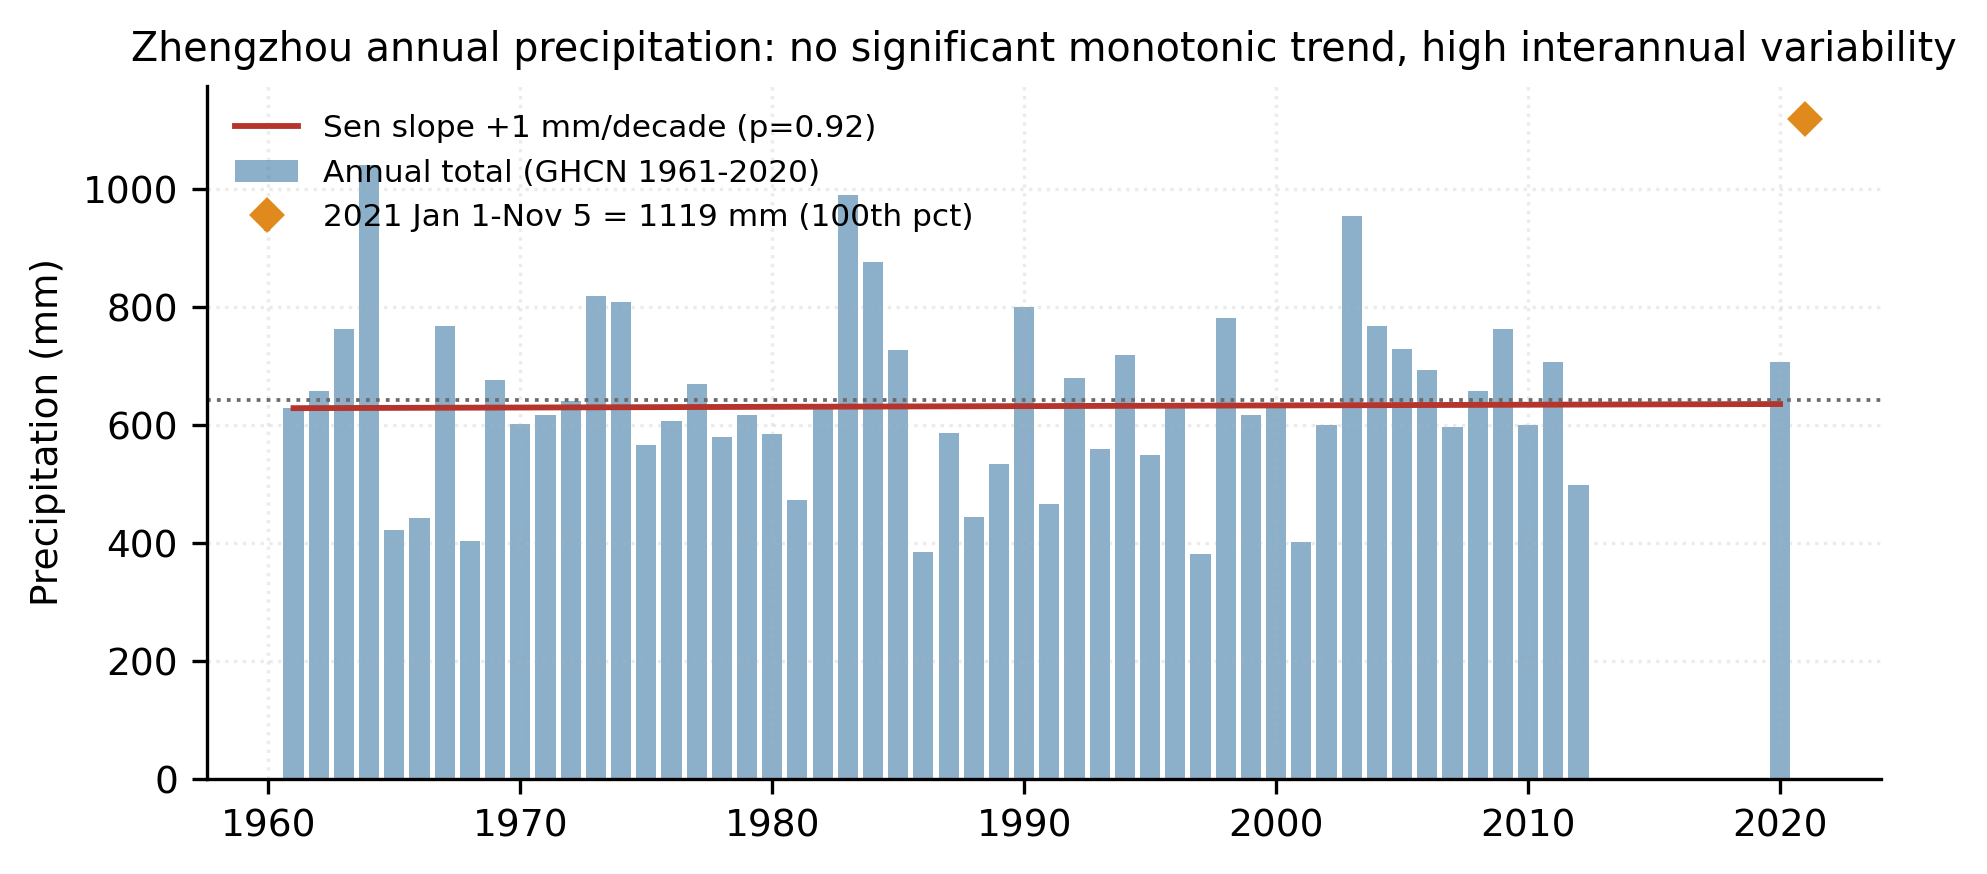
\includegraphics[width=0.42\linewidth]{../02_figures/fig01_annual_total.png}
\caption{Annual precipitation at Zhengzhou, 1951--2024. The Sen line is fitted on 1961--2020; the 2021 diamond (1\,119.4\,mm for January--5 November) lies far above the fitted distribution of the 53 complete years.}
\label{fig:annual}
\end{figure}

\subsection{Return levels and the rarity of the event}

A generalised extreme value distribution $F(x)=\exp\{-[1+\xi(x-\mu)/\sigma]^{-1/\xi}\}$ \cite{coles2001} is fitted by maximum likelihood to the 53 annual daily maxima of 1961--2020; the shape estimate is $\xi=-0.026$, i.e.\ a light upper tail close to the Gumbel case, and Section~\ref{sec:eval} shows how little this parameter is identified. Confidence intervals come from a parametric bootstrap with 1\,000 replicates for the return levels and 500 (300 for the official 449\,mm) for the event return periods, with a fixed seed. Table~\ref{tab:q1rl} gives the return levels.

\begin{table}[H]
\centering
\caption{Return levels of daily precipitation at Zhengzhou (mm), GEV fitted on 1961--2020, with bootstrap 95\% intervals.}
\label{tab:q1rl}
\footnotesize
\setlength{\tabcolsep}{3pt}
\begin{tabular}{lrrrrrr}
\toprule
$T$ (yr) & 2 & 5 & 10 & 20 & 50 & 100\\
\midrule
Level (mm) & 78.0 & 106.3 & 124.5 & 141.7 & 163.4 & 179.4\\
95\% CI & [69.3, 87.0] & [95.1, 118.6] & [109.1, 140.5] & [120.3, 165.3] & [132.0, 204.7] & [139.2, 242.5]\\
\bottomrule
\end{tabular}
\end{table}

The 20 July 2021 daily total of 188.7\,mm exceeds the 100-year level. Its empirical return period, read from the 54 complete years that precede it, is 54\,yr; the fitted GEV assigns 151\,yr. The difference is instructive: an event of this size was not unprecedented in the daily record (1978 reached 189.4\,mm), so a naive daily analysis would classify 2021 as rare but plausible and stop there. The three-day total of 313.4\,mm is another matter: it is the largest in 71 years of record, and the fitted three-day GEV places it at $6.4\times10^{3}$\,yr. For the official three-day total of 449\,mm the fitted model returns $1.6\times10^{8}$\,yr, reported only to make a point: above roughly the 200-year level the extrapolation is dominated by the uncertain shape parameter, and the interval spans 678\,yr to infinity. The honest statement is that 449\,mm in 72\,h lies outside the range in which a 53-year record can discriminate between return periods; the practical conclusion does not depend on the exact number, because the event exceeded every standard in force by a factor of three or more.

\subsection{Wet years}

The five wettest years in 1961--2020, expressed as standardised anomalies, are 1964 (1\,041.3\,mm, $z=2.69$), 1983 (990.6\,mm, $z=2.35$), 2003 (953.9\,mm, $z=2.10$), 1984 (877.4\,mm, $z=1.58$) and 1973 (819.6\,mm, $z=1.19$). Their spacing is irregular, consistent with the absence of a change point: wet years are a stationary tail phenomenon, not a regime. The 2021 year, even truncated at 5 November, reaches 1\,119.4\,mm ($z=3.46$) and is the wettest year in the 71-year GHCN record.

\subsection{Quantifying the waterlogging event}

Rainfall becomes a disaster through runoff. We estimate the storm-water volume with the SCS curve-number method \cite{neh1986}, $Q=(P-0.2S)^2/(P+0.8S)$ with $S=25400/\mathrm{CN}-254$, applied to the 1\,180\,km$^2$ built-up area of Zhengzhou. Antecedent wetness in July 2021 was high, so we bracket the curve number between 75 and 95; the central case is CN\,85, appropriate to a dense urban surface with partial sewer connection. Over the event window the areal rainfall is 313.4\,mm, giving a runoff depth of 265.4\,mm and a volume of $3.13\times10^{8}$\,m$^3$; at the official 449\,mm the volume is $4.71\times10^{8}$\,m$^3$. Table~\ref{tab:cn} shows the sensitivity.

\begin{table}[H]
\centering
\caption{Runoff response of the 1\,180\,km$^2$ urban area to the July 2021 storm (SCS-CN).}
\label{tab:cn}
\small
\begin{tabular}{lrrrrr}
\toprule
Curve number & 75 & 80 & 85 & 90 & 95\\
\midrule
Runoff depth (mm) & 230.6 & 248.3 & 265.4 & 281.9 & 297.9\\
Volume ($10^{8}$\,m$^3$) & 2.72 & 2.93 & 3.13 & 3.33 & 3.52\\
\bottomrule
\end{tabular}
\end{table}

The failure mechanism is a capacity mismatch in time, not in volume alone. The peak hour delivered 201.9\,mm\,h$^{-1}$; the one-year design intensity of the Zhengzhou network is about 36\,mm\,h$^{-1}$, the two-year 43 and the three-year 50. The peak therefore exceeded design capacity by factors of 5.6, 4.7 and 4.0. Routing that hour through the same curve-number model gives 156.6\,mm of runoff, of which 120.6\,mm lies above the one-year capacity --- $1.4\times10^{8}$\,m$^3$ arriving within sixty minutes. Clearing the three-day event (313.4\,mm of rain, 265.4\,mm of runoff) at full capacity takes 7.4\,h at the one-year standard and 5.3\,h at the three-year standard, and during that time surface water continues to accumulate in underpasses, basements and the metro. This is why the loss was concentrated in underground space: the network was not merely overloaded, it was overloaded for a full working day. The daily structure of the event, its monthly context and its return periods are plotted in Appendix~\ref{app:extrafig}.

\section{Task 2: a national trend map}\label{sec:q2}

\subsection{Design}

For each of the 25 cities we compute the same annual indices as in Section~\ref{sec:q1} and test the same five trends. Five hypotheses on 25 cities is 125 tests, and at a nominal 5\% level roughly six would be significant by chance alone. Reporting those six as ``trends'' is the most common error in this literature, so we control the false discovery rate with the Benjamini--Hochberg procedure \cite{bh1995} and report only discoveries with $q\le0.05$. Because the six indices are tested on the same 25 series we pool them into one family: five indices over 25 cities plus the threshold count over the 21 cities where it is defined, i.e.\ 146 finite tests. Controlling each index separately over its own cities would be less conservative and would return 1, 1, 1, 11 and 13 discoveries instead of 2, 1, 1, 7 and 9. We report the pooled family, and we also report the median Sen slope, because the median is not distorted by the few cities with very large trends.

\subsection{What actually trends}

The pattern is sharply selective (Table~\ref{tab:q2sig}). Annual totals trend in only two cities, and the one-day maximum in one. In contrast, seven cities have a significant trend in daily intensity and nine in the number of wet days. A national signal that appears in frequency and intensity but not in totals is the spatial analogue of the Zhengzhou result: rainfall is being redistributed within the year rather than increased.

\begin{table}[H]
\centering
\caption{National trend summary, 25 cities, 1961--2020, Benjamini--Hochberg $q\le0.05$.}
\label{tab:q2sig}
\footnotesize
\setlength{\tabcolsep}{4pt}
\begin{tabular}{lrrr}
\toprule
Index & Sig. & Median Sen & Range of Sen\\
\midrule
Total (mm) & 2 & $+3.13$ & $-36.5$ to $+60.5$\\
Rx1day (mm) & 1 & $+1.00$ & $-4.19$ to $+13.51$\\
R95p (mm) & 1 & $-1.01$ & $-22.2$ to $+17.3$\\
SDII (mm\,d$^{-1}$) & 7 & $+0.240$ & $+0.047$ to $+0.867$\\
Wet days (d) & 9 & $-2.50$ & $-10.96$ to $+2.22$\\
Days $\ge50$\,mm (\% dec$^{-1}$) & 0 & $+2.71\%$ & $-15.3\%$ to $+9.1\%$\\
\bottomrule
\end{tabular}
\end{table}

Two entries in Table~\ref{tab:q2sig} deserve emphasis. First, the SDII slope is positive in all 25 cities, with a median of $+0.24$\,mm\,d$^{-1}$ per decade: although only seven are individually significant, the sign is unanimous, which is much stronger evidence than any single test. Second, the threshold-count trends are noisy and none survives FDR control, so we do not claim a national increase in heavy-rain days.

The extremes of the distribution of trends are worth naming. Haikou has the largest increase in Rx1day ($+13.51$\,mm\,dec$^{-1}$, $q=0.23$), Wuhan $+5.83$ ($q=0.29$) and Jinan $+3.51$ ($q=0.46$); Beijing has the largest decrease ($-4.19$\,mm\,dec$^{-1}$, $q=0.23$). Nanning's R95p falls by 22.2\,mm\,dec$^{-1}$, Kunming by 14.2 and Beijing by 15.1. None of these individual slopes survives FDR control except Urumqi's Rx1day increase ($+3.33$\,mm\,dec$^{-1}$, $q<0.01$), which is a reminder that a large slope on a short record is not evidence.

\subsection{Regional structure}

Pooling cities into six belts (North China, Northeast, Yangtze, South, Northwest, Southwest) shows that the sign of the total-rainfall trend is regional, not national: North China $-6.4$\,mm\,dec$^{-1}$, Northeast $+4.6$, Yangtze $+20.2$, South $+21.5$, Northwest $+12.5$, Southwest $-27.1$. Wet-day counts fall in every belt, which is why the national median wet-day slope is negative while the national median total slope is positive. A policy that reads only the national mean would conclude that nothing is happening.

\begin{figure}[H]
\centering
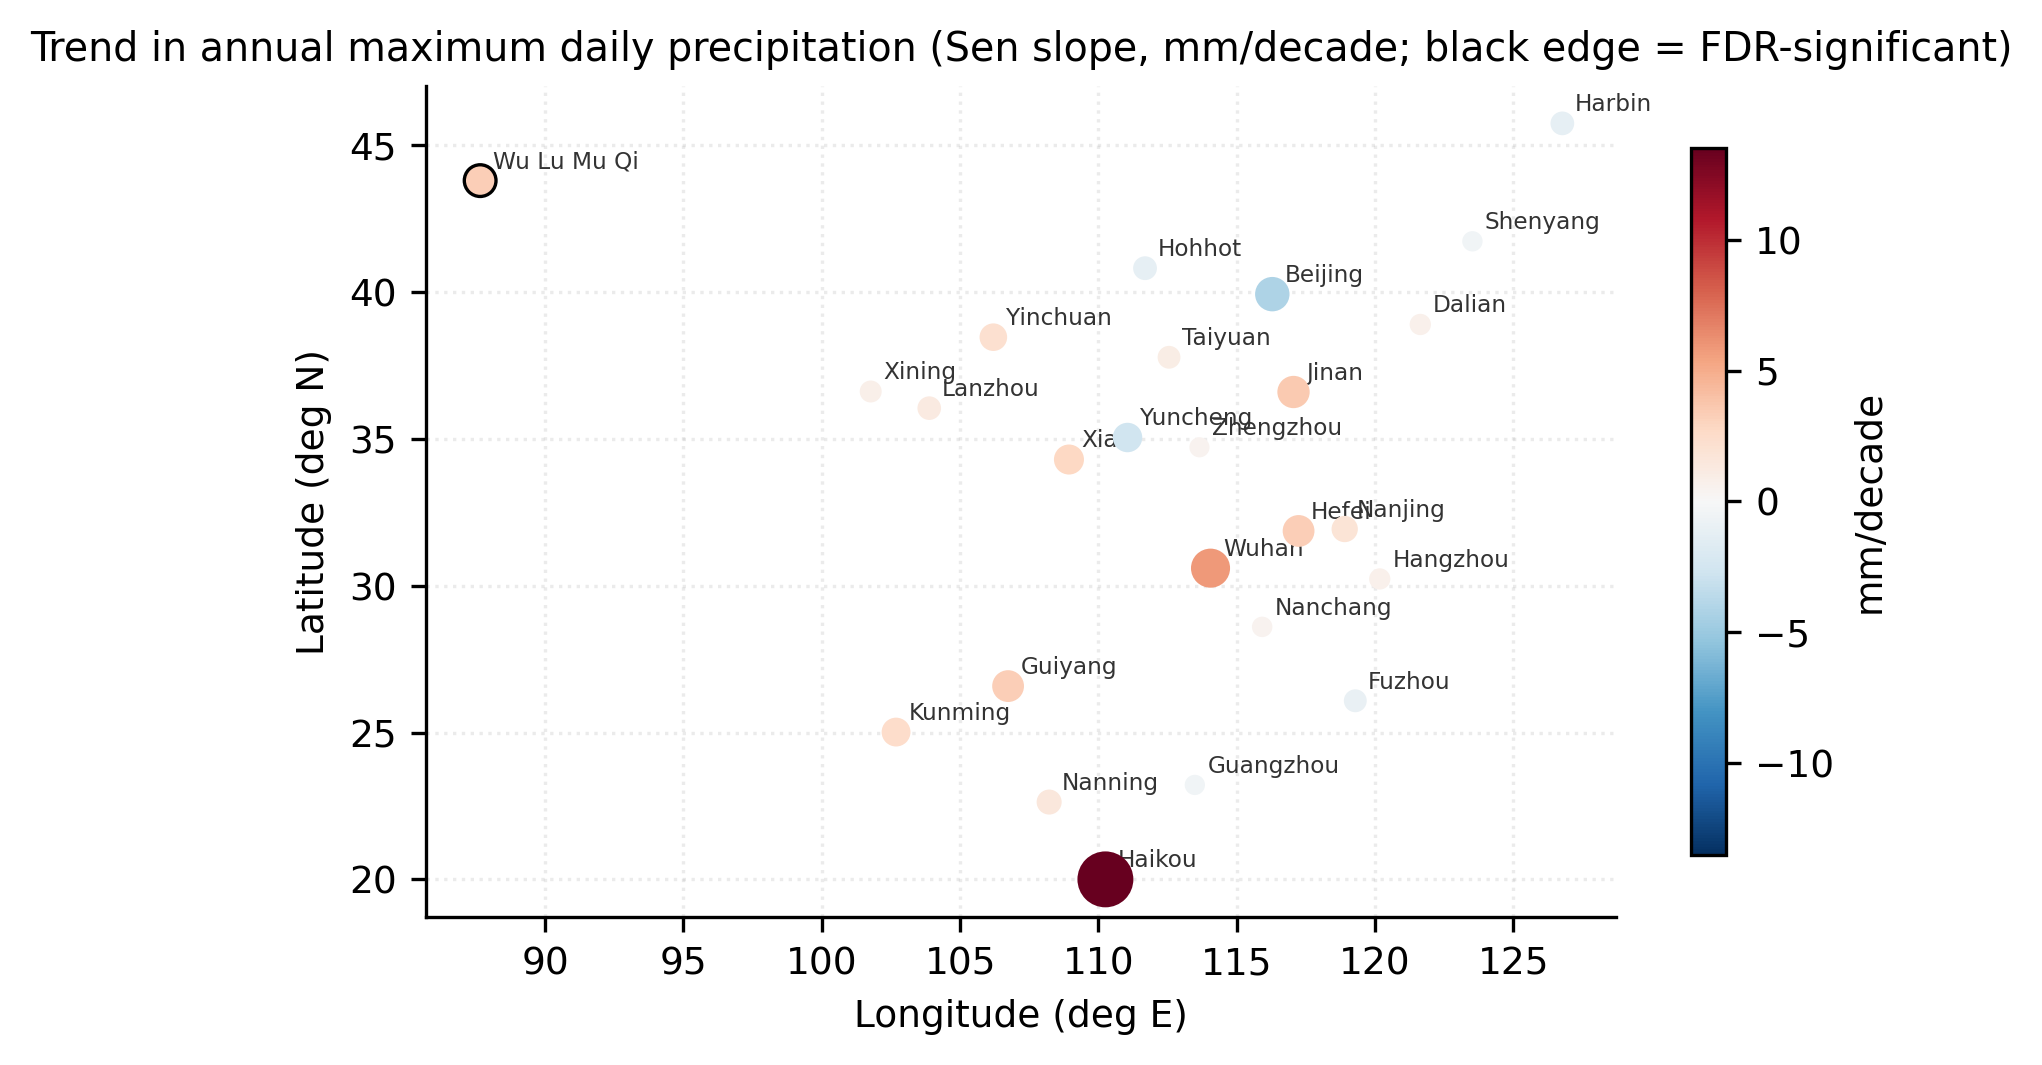
\includegraphics[width=0.38\linewidth]{../02_figures/fig07_trend_map_rx1day.png}
\caption{Sen slope of annual maximum one-day rainfall (mm per decade) for the 25 cities; red denotes increasing extremes and blue decreasing. Circle size scales with the absolute slope.}
\label{fig:maprx}
\end{figure}

\subsection{Classification}

To avoid imposing a geographical partition, we cluster the cities on five standardised trend features (Rx1day, total, R95p, SDII, days $\ge50$\,mm) plus mean intensity, with $k$-means and $k$ chosen by silhouette. The optimum is $k=2$ (silhouette 0.336; $k=3$ gives 0.238), and the two clusters are geographically coherent:

\begin{itemize}[leftmargin=1.4em,itemsep=1pt]
\item \textbf{Cluster 0 (17 cities, continental):} mean annual total 602\,mm and mean Rx1day 63.4\,mm; per decade the Rx1day trend is $+0.80$\,mm, the total trend $-4.66$\,mm, the R95p trend $-4.10$\,mm and the count of days above 50\,mm changes by $-1.85\%$.
\item \textbf{Cluster 1 (8 cities, humid south):} mean annual total 1\,389\,mm and mean Rx1day 113.8\,mm; per decade the Rx1day trend is $+3.03$\,mm, the total trend $+34.2$\,mm, the R95p trend $+4.36$\,mm and the count of days above 50\,mm rises by $+6.49\%$.
\end{itemize}

The split is not a restatement of latitude: it says that the humid south is both wetter and becoming more extreme, whereas the continental interior is drying in total but not becoming less extreme per event. The city-by-index matrix, the cluster geometry and the regional anomaly series are shown in Appendix~\ref{app:extrafig}. This is the input to the risk ranking of Section~\ref{sec:q3}.
\section{Task 3: predicting which city breaks its record next}\label{sec:q3}

\subsection{Problem formulation}

The task says ``predict which cities may experience extreme precipitation''. Any comparison of methods is meaningless until the predictand is fixed, and the choice of predictand turns out to be more consequential than the choice of model. We therefore state the problem as a genuine forecast: using only 1961--2010, predict each city's largest daily rainfall in the held-out window 2011--2024.

The held-out window is not the nominal 14 years. Because of the 300-valid-day rule (Section~\ref{sec:data}), a city contributes 5, 6 or 7 test years (18 cities give 7, two give 6, three give 5); Zhengzhou contributes 2011, 2012 and 2020--2024. The forecast horizon is therefore $n_{\text{test}}$ years per city, and every method is evaluated against the same realized maximum. Twenty-three cities pass the training requirement of at least 40 valid years in 1961--2010 and at least 5 in 2011--2024.

\subsection{Ten strategies}

All strategies are fitted on the training window only.

\textbf{Extreme-value family.} Seven variants share a GEV \cite{coles2001} or Gumbel fit to the annual maxima: (i) the $T$-year quantile with $T$ equal to the city's test length, fitted by maximum likelihood; (ii) the same quantile fitted by L-moments \cite{hosking1985}, which is more stable on short records; (iii) the \emph{expected maximum} of the next $n$ years, $\mathbb{E}[M_n]=\int_0^1 F^{-1}(u^{1/n})\,du$ by adaptive quadrature, the statistic that minimises mean squared forecast error when the predictand is a maximum and which exceeds the $n$-year quantile by $0.577\sigma$ under a Gumbel tail, so a quantile target is biased low; (iv) the expected maximum with the location shifted by the Sen slope over the 32-year gap between window midpoints; (v) a peaks-over-threshold model with the threshold at the wet-day 95th percentile, three-day declustering and a Poisson--GPD return level; (vi) and (vii) the quantile and the trend quantile under $\xi=0$.

\textbf{Regression and classification family.} Each city is described by thirteen features (mean annual total, mean and standard deviation of Rx1day, its Sen slope, the R95p slope, SDII, wet days, days $\ge50$\,mm, latitude, longitude, elevation, training years). Ridge, random forest and gradient boosting regress the realized maximum on these features with leave-one-city-out cross-validation, so no city is predicted by a model that has seen it; for the binary question ``will this city exceed its training record?'' we add the GEV exceedance probability $\Pr(M_T>x_{\text{record}})$ with both estimators plus the same three learners.

\subsection{Results}

Table~\ref{tab:q3} reports the comparison. Four findings stand out.

\begin{table}[H]
\centering
\caption{Held-out forecast of each city's maximum daily rainfall, 23 cities. Bias is prediction minus observation. Overlap counts how many of the five largest predicted values are among the five largest observed.}
\label{tab:q3}
\small
\begin{tabular}{lrrrrrr}
\toprule
Method & RMSE (mm) & MAE (mm) & $R^2$ & Spearman & Bias (mm) & Overlap\\
\midrule
GEV, $T$-year quantile (MLE) & 64.8 & 45.5 & 0.242 & 0.747 & $-41.5$ & 4\\
GEV, $T$-year quantile (L-moment) & 66.0 & 46.5 & 0.213 & 0.748 & $-42.2$ & 4\\
\textbf{GEV, expected maximum} & \textbf{55.7} & \textbf{39.6} & \textbf{0.440} & \textbf{0.746} & $-20.5$ & 4\\
GEV, expected maximum + trend & \textbf{53.9} & \textbf{38.5} & \textbf{0.475} & 0.688 & $-17.4$ & 3\\
GPD peaks-over-threshold & 70.6 & 49.3 & 0.099 & 0.735 & $-45.8$ & 3\\
Gumbel, quantile & 65.6 & 45.8 & 0.223 & 0.739 & $-39.8$ & 4\\
Gumbel, quantile + trend & 62.9 & 44.7 & 0.286 & 0.743 & $-36.7$ & 4\\
Ridge regression & 61.8 & 43.6 & 0.310 & 0.643 & $-1.2$ & 3\\
Random forest & 63.8 & 48.9 & 0.265 & 0.613 & $+6.4$ & 1\\
Gradient boosting & 66.3 & 51.4 & 0.207 & 0.598 & $+5.8$ & 2\\
\bottomrule
\end{tabular}
\end{table}

\textbf{(1) The target dominates the model.} Moving from a $T$-year quantile to the expected maximum of $n$ years reduces RMSE from 64.8 to 55.7\,mm and halves the bias ($-41.5$ to $-20.5$\,mm), with the same data and the same distribution; a paired bootstrap over cities puts the RMSE gain at $[3.3, 13.6]$\,mm, so the improvement is not sampling noise. A quantile is systematically too high for a maximum; this is a bias of definition, not of fit, and it explains why so many published ``predictions'' are over-confident.

\textbf{(2) Trends help levels and hurt ranks.} The trend-shifted variant achieves the best RMSE (53.9\,mm) and the best $R^2$ (0.475) but its Spearman correlation falls from 0.746 to 0.688 and its top-five overlap from 4 to 3; the RMSE gain over the stationary expected maximum is only 1.7\,mm, with a bootstrap interval of $[-1.9, 7.0]$ that straddles zero. The reason is that a Sen slope estimated on 50 years is noisy; using it to shift a level adds variance that helps on average but reshuffles the ranking. We therefore use the stationary model to \emph{rank} cities and the trend model to report \emph{levels}, and we say so explicitly rather than hiding the trade-off.

\textbf{(3) Extreme-value theory beats machine learning on ranking.} Seven EVT variants have Spearman correlations of 0.69--0.75 and top-five overlaps of 3/5 or 4/5; the best machine-learning model reaches 0.643 with 3/5, the weakest 0.598 with 2/5, and one model orders only 1/5. The regression family is competitive on RMSE but poor at ordering, because it regresses towards the mean of the feature space and compresses the extremes. The complementarity is real: machine learning removes the bias ($-1.2$\,mm for Ridge) while EVT preserves the ordering. A hybrid that ranks with EVT and calibrates the level with a regression is the sensible product, and the numbers in Table~\ref{tab:q3} say why neither alone is enough.

\textbf{(4) MLE becomes pathological on short records.} Guangzhou's MLE fit returns a 50-year level of 450\,048\,mm, because a single very large annual maximum pushes the shape parameter into the heavy-tail region where the return level explodes. The L-moment fit on the same data gives 268.3\,mm. We flag such fits automatically (a 50-year level more than three times the observed record) rather than reporting them.

For the classification task the GEV exceedance probability with MLE parameters is best (AUC 0.833, Brier 0.143, accuracy 0.826), followed by the L-moment version (0.756, 0.174, 0.783) and logistic regression (0.178, 0.227, 0.783). The two tree ensembles fail (AUC 0.522 and 0.178): with 23 cities and five positives, a tree cannot learn a decision boundary without overfitting the folds.

\subsection{Which cities, and which records broke}

Five cities exceeded their 1961--2010 record in the held-out window (Table~\ref{tab:records}). None of them is Zhengzhou, and none of the breaks happened in 2021. This is the most important negative result in the paper: a daily-index screen would have assigned Zhengzhou a moderate risk, because its 2021 daily total (188.7\,mm) did not even beat its 1978 value (189.4\,mm). The extremity of that disaster lived at the hourly and three-day scales, which the annual-maximum machinery does not see. We keep the daily screen, because it is the only one available for 25 cities, but we state its blind spot and carry it into the recommendations of Section~\ref{sec:q5}.

\begin{table}[H]
\centering
\caption{Cities that broke their 1961--2010 daily record during the held-out window.}
\label{tab:records}
\small
\begin{tabular}{lrrrr}
\toprule
City & Training record (mm) & Held-out max (mm) & Year & Test years\\
\midrule
Harbin & 123.7 & 146.6 & 2012 & 7\\
Urumqi & 57.7 & 89.9 & 2020 & 6\\
Yinchuan & 87.1 & 113.3 & 2012 & 7\\
Fuzhou & 195.6 & 357.6 & 2023 & 7\\
Haikou & 327.9 & 331.2 & 2011 & 5\\
\bottomrule
\end{tabular}
\end{table}

\subsection{Regional pooling: is one growth curve admissible?}

Every prediction above rests on fifty annual maxima and a five-to-seven-year hold-out, so at-site parameters are noisy. Index-flood pooling \cite{hosking1997} borrows strength across sites: divide each city's annual maxima by its mean, pool the scaled series, fit one regional GEV by L-moments, and multiply the growth curve back by the site index \cite{hosking1985}. On the 23 cities the growth curve is $0.916$, $1.525$ and $2.138$ at 2, 10 and 50 years. Whether it may be applied nationally is testable, and the Hosking--Wallis test rejects it: with 400 simulated homogeneous regions $H_1=2.56$, $H_2=-0.68$, $Z=-0.39$, and $H_1>2$ marks a heterogeneous region. Pooling still shaves the expected-maximum error from $55.7$ to $54.5$\,mm, but it forces one curve on every city, so the $p_{10}$ ranking drifts from the at-site one ($\rho=0.545$).

The test also says what the correct pooling unit is. Grouping the cities by their own L-moment ratios (L-CV, L-skew and the log index, $k=2$) yields two groups of 12 and 11 sites (the heterogeneity statistic is Hosking and Wallis \cite{hosking1993}) with $H_1=0.22$ and $0.03$, both comfortably homogeneous, a growth curve of $1.566$ and $1.473$ at ten years, an error of $56.3$\,mm and a ranking that stays close to the at-site one ($\rho=0.843$). The honest summary is therefore narrow: pooling buys at most $1.2$\,mm of level accuracy, because the error is dominated by the five record-breaking cities, but it is admissible only group-wise, and the ranking should stay at-site. We report the grouped curve as a short-record fallback, not as a replacement.

\subsection{Risk ranking}

Combining the expected maximum, the $T$-year level and the exceedance probability gives the ranking in Table~\ref{tab:risk}. The humid south dominates the top of the list: Fuzhou, Haikou and Guangzhou, which is exactly the cluster that Section~\ref{sec:q2} found to be intensifying. Two continental cities intrude, Hohhot and Yuncheng, not because their rainfall is large but because a short, variable record makes an existing record easier to beat in relative terms. Zhengzhou is a deliberate counter-example: it ranks sixteenth by $p_{10}=0.073$ and tenth on the composite, the mean of its rank by $p_{10}$ and by the regression ten-year maximum (170.1\,mm), because its 1961--2010 record of 189.4\,mm already sits high inside a light-tailed local distribution. Probability alone therefore does not flag the city that suffered the disaster, which is the quantitative reason why Sections~\ref{sec:q4} and~\ref{sec:q5} add exposure and vulnerability to the hazard layer.

\begin{table}[H]
\centering
\caption{Ten-year probability $p_{10}$ of exceeding the 1961--2010 daily record, from the L-moment GEV fit, with that fit's 10- and 50-year return levels and the regression estimate of the ten-year maximum.}
\label{tab:risk}
\small
\begin{tabular}{lrrrr}
\toprule
City & $p_{10}$ & RL10 (mm) & RL50 (mm) & Regression ten-year max (mm)\\
\midrule
Fuzhou & 0.283 & 172.2 & 247.8 & 288.7\\
Haikou & 0.248 & 260.9 & 358.7 & 296.7\\
Guangzhou & 0.230 & 184.6 & 268.3 & 205.1\\
Hohhot & 0.210 & 86.5 & 129.9 & 82.8\\
Yuncheng & 0.170 & 89.3 & 140.0 & 94.4\\
Nanjing & 0.170 & 154.7 & 203.7 & 219.8\\
Dalian & 0.165 & 149.6 & 219.9 & 161.7\\
Urumqi & 0.162 & 49.0 & 82.6 & 92.5\\
Wuhan & 0.162 & 182.2 & 286.9 & 199.4\\
Nanning & 0.132 & 150.0 & 208.3 & 174.1\\
\bottomrule
\end{tabular}
\end{table}

The same probabilities are mapped in Appendix~\ref{app:extrafig} (Figure~\ref{fig:riskmap}).

\section{Task 4: two storms, one word}\label{sec:q4}

\subsection{Event windows and indices}

We compare the Zhengzhou storm (17--23 July 2021) with the Shanxi storm (1--7 October 2021). For Shanxi we use Taiyuan, which lies in the core of the rain belt, and Yuncheng plus the attachment station 53975099999, which lie on its southern margin; provincial aggregates come from the official reports. Six indices describe each event: total rainfall, one-day maximum, three-day maximum, the longest run of consecutive wet days, the ratio of one-day to three-day rainfall (a concentration measure), and the percentile of that ratio within the station's own climatology. Return periods are computed from the station's 1961--2020 GEV fit.

\begin{table}[H]
\centering
\caption{Event indices. Return periods are GEV estimates; the percentile of the concentration ratio is computed from each station's own annual records.}
\label{tab:q4event}
\small
\begin{tabular}{lrrrrrr}
\toprule
 & Total & 1-day max & 3-day max & Wet run & 1d/3d & RP(1d)\\
 & (mm) & (mm) & (mm) & (days) & ratio & (years)\\
\midrule
Zhengzhou & 362.2 & 188.7 & 313.4 & 5 & 0.60 & 134.5\\
Taiyuan & 203.2 & 85.6 & 182.9 & 5 & 0.47 & 9.5\\
Yuncheng & 52.6 & 18.3 & 39.9 & 4 & 0.46 & 1.0\\
Station 53975 & 26.9 & 10.9 & 20.8 & 4 & 0.52 & 1.0\\
\bottomrule
\end{tabular}
\end{table}

The two core stations differ by a factor of 14 in the rarity of their daily rainfall (134.5 versus 9.5 years) but agree in duration (five consecutive wet days). Zhengzhou's daily total contains 60\% of its three-day total, Taiyuan's only 47\%, and Taiyuan's concentration ratio sits at the 6.5th percentile of its own climatology, i.e.\ the storm was unusually \emph{even} for that station. The southern stations received an order of magnitude less rain, confirming that the October event was concentrated in a narrow belt along the Taihang mountains rather than spread over the province.

\subsection{Are they the same type?}

We formalise the comparison with three criteria, each scaled to be dimensionless:

\begin{enumerate}[leftmargin=1.4em,itemsep=1pt]
\item \emph{Rarity ratio}: $\mathrm{RP}_{1d}(\text{Zhengzhou})/\mathrm{RP}_{1d}(\text{Taiyuan})=14.1$. A ratio above 3 means the two events are not drawn from the same rarity class.
\item \emph{Concentration gap}: $|0.602-0.468|=0.134$ (0.13 at printed precision). A gap above 0.10 means the temporal profiles differ materially.
\item \emph{Duration gap}: both events have a five-day wet run, so this criterion contributes 0.
\end{enumerate}

Two of the three criteria fail, so the answer is \textbf{no}: the Zhengzhou storm is an \emph{intensity-type} event and the Shanxi storm is a \emph{persistence-type} event. The distinction is not academic. Intensity-type events are governed by the peak hour and by the capacity of drainage and of underground space; persistence-type events are governed by cumulative volume, by slope stability and by the saturation of reservoirs and soils. A city that has upgraded only its pipes is prepared for neither, and a city that has prepared for a 1-in-100 year daily total may still be destroyed by a 1-in-10 year daily total that lasts four days.

\begin{figure}[H]
\centering
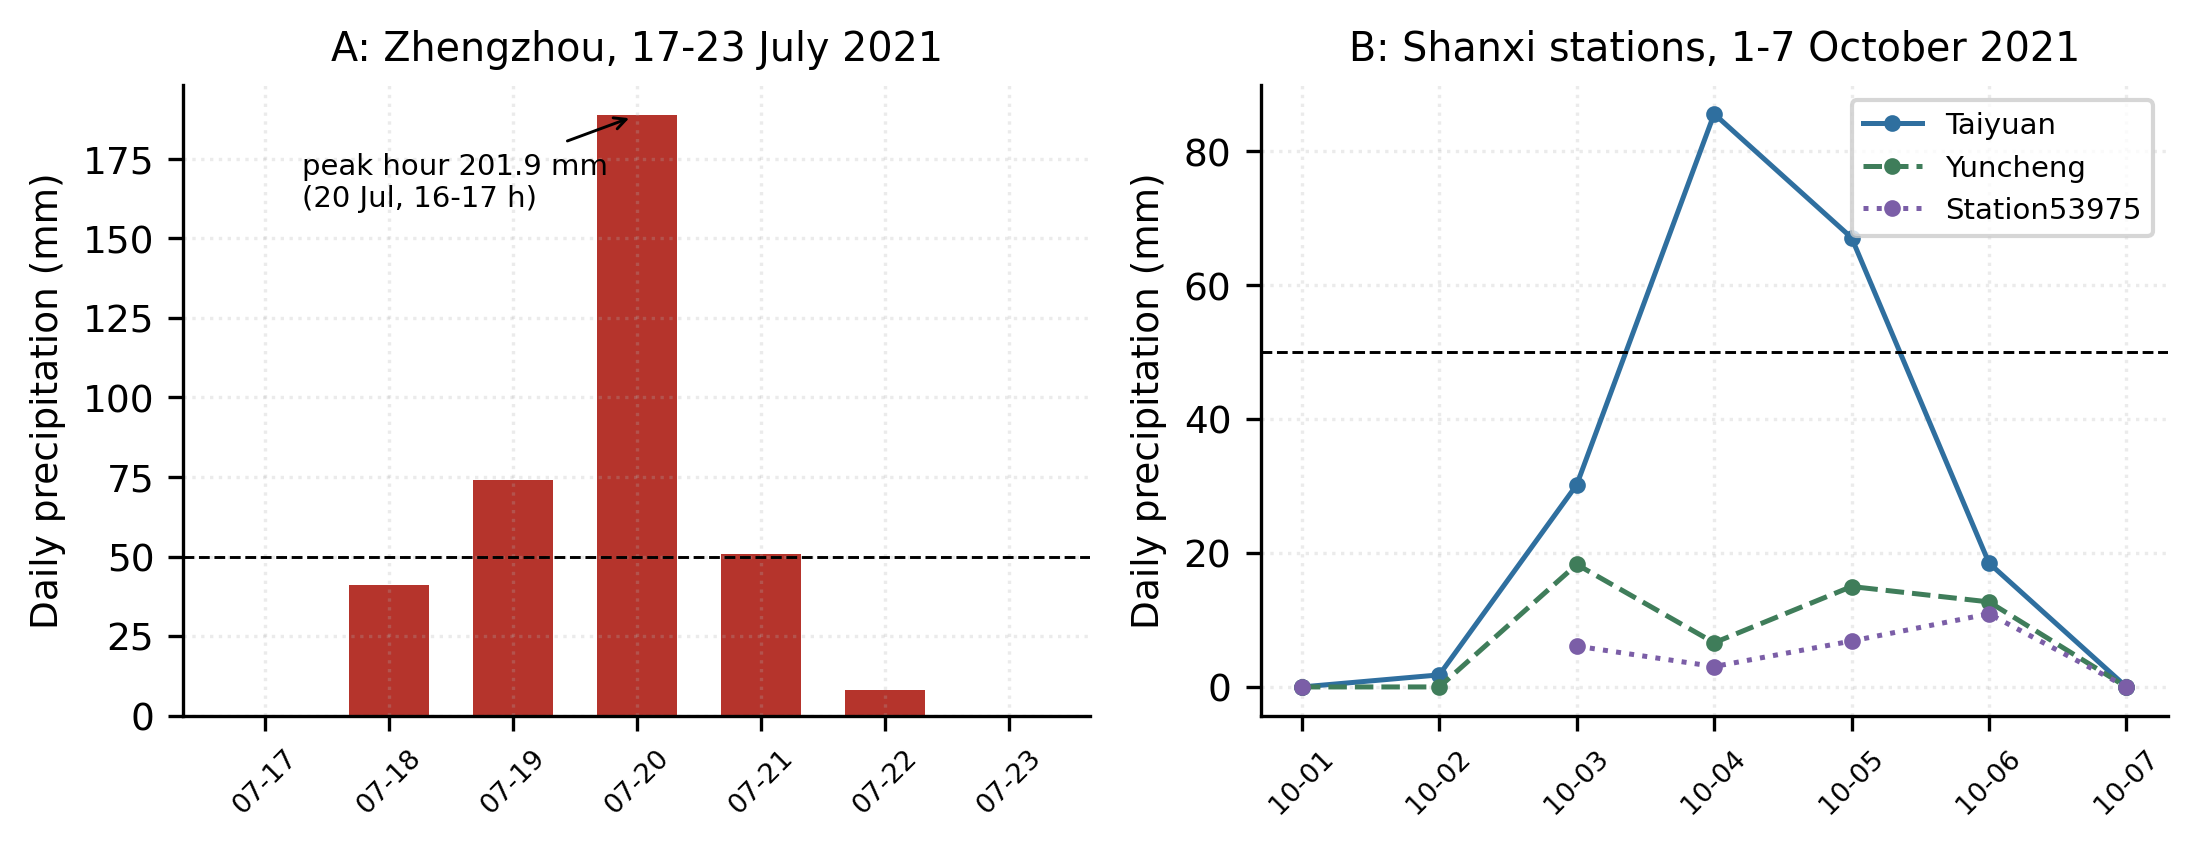
\includegraphics[width=0.38\linewidth]{../02_figures/fig16_hyetograph.png}
\caption{Daily hyetographs: (A) Zhengzhou, 17--23 July 2021, with the 201.9\,mm peak hour annotated; (B) Taiyuan, Yuncheng and station 53975, 1--7 October 2021.}
\label{fig:hyeto}
\end{figure}

\subsection{Why the losses differ by a factor of 24}

Two loss figures circulate for Henan. The problem statement quotes 655 billion CNY, a preliminary count for Zhengzhou as of 23 July 2021; the State Council investigation closed in January 2022 with 409.0 billion CNY for the municipality and 1\,200.6 billion CNY for the province \cite{sc}. We adopt the audited figures because they cover the whole event rather than its first three days, and compare provinces so that numerator and denominator come from one assessment. Table~\ref{tab:q4loss} assembles the official loss figures and normalises them. The raw ratio (23.9) is misleading because the two provinces differ in area, population and exposure. Normalising by area gives 22.4, by affected population 2.84 and by population 8.36; the raw 23.9 is the area-normalised 22.4 multiplied by the area ratio (167\,000/156\,700\,km$^2$ = 1.07). A per-millimetre ratio (6.4) is indicative only, because the two events are measured with different rainfall denominators.

\begin{table}[H]
\centering
\caption{Official losses and normalisations. Loss in $10^8$ CNY; area in km$^2$; population in millions.}
\label{tab:q4loss}
\small
\begin{tabular}{lrrr}
\toprule
 \textbf{Item} & Zhengzhou city & Henan province & Shanxi province\\
\midrule
Direct loss ($10^8$ CNY) & 409.0 & 1\,200.6 & 50.29\\
Area (km$^2$) & 7\,567 & 167\,000 & 156\,700\\
Population (millions) & 12.60 & 99.37 & 34.80\\
Affected (millions) & -- & 14.786 & 1.757\\
Deaths and missing & 380 & 398 & 18\\
\midrule
Loss per km$^2$ ($10^4$ CNY) & 540.5 & 71.9 & 3.2\\
Loss per affected (CNY) & -- & 8\,120 & 2\,862\\
Deaths per million affected & -- & 26.9 & 10.2\\
\bottomrule
\end{tabular}
\end{table}

The decomposition is an identity, not a causal test: it locates the 22-fold gap in three measurable factors rather than attributing it to rainfall. Rainfall depth explains only a factor of 2.2 (449\,mm against 203\,mm at the core stations). The remaining order of magnitude is exposure and vulnerability: Henan's plain is 2.7 times denser than Shanxi's plateau margin, the share of the provincial population affected was three times larger (14.9\% versus 5.1\%), and each affected person lost 2.8 times more, which reflects the destruction of underground space, the metro, and the fact that Zhengzhou's warning and evacuation were demonstrably too slow (the State Council report \cite{sc} documents 139 concealed deaths and a failure to suspend the metro and tunnel operations). For a planner, the lesson is that the same rainfall over a denser, more underground-dependent city produces several times the loss; reducing exposure is as effective as reducing hazard.

A multiplicative identity still leaves the question of which factor to blame, and the answer depends on the order in which the factors are switched. Averaging over all orderings settles it: with the four factors as players and their partial products as coalition worth, the Shapley value divides the 23.9-fold gap into population density $31.3\%$, affected share $33.6\%$, loss per affected person $32.7\%$ and area $2.5\%$, and the identity closes to $4\times10^{-15}$. Splitting the logarithm instead gives $31.1$, $34.1$, $32.9$ and $2.0\%$; the two conventions answer the ratio question and the level question, and neither changes the message. Single-factor removal is sharper: delete density and the gap is still $8.9$, delete the affected share $8.1$, delete severity $8.4$, delete the area ratio $22.4$. No single social factor carries the result, so the conclusion survives whichever factor a reader finds most contestable; area is irrelevant. Appendix~\ref{app:extrafig} plots the underlying normalisations (Figure~\ref{fig:lossnorm}).

\section{Task 5: what to build, where, and in what order}\label{sec:q5}

\subsection{From hazard to a decision variable}

A construction plan is an allocation of money across measures, so the model must price risk. We use a three-day event scale throughout, because that is the scale at which the two storms of Section~\ref{sec:q4} caused damage.

\textbf{Hazard.} For each city, annual maximum three-day rainfall $X$ is fitted with a GEV by L-moments over 1961--2020. The design depth for a $T$-year standard is $\mathrm{RL}_{3d}(T)$; for Zhengzhou it is 102.9\,mm at $T=2$, 162.3\,mm at $T=10$ and 207.2\,mm at $T=50$, against an observed 2021 value of 313.4\,mm (station) and 449\,mm (official).

Two accounting conventions coexist here and answer different questions. Task~1 asks how much water arrives in the peak window and how long the network needs to clear it; Task~5 asks what a year of rainfall costs, so it routes the 72-hour total through the same curve-number model and prices the resulting volume against capacity. The Task~1 peak-hour excess of $1.4\times10^{8}$\,m$^3$ and the Task~5 event budget of $3.50\times10^{8}$\,m$^3$ are therefore not interchangeable.

\textbf{Capacity and damage.} Capacity is $C=\mathrm{RL}_{3d}(T)+S_{\text{sto}}$, the design rainfall depth plus the depth equivalent of distributed storage $S_{\text{sto}}$. Both the hazard and the overflow are measured in \emph{runoff} space: the three-day total $X$ is routed through the SCS-CN curve, whose retention is $S_{\text{ret}}=25400/\mathrm{CN}-254$, to give $Q(X)$, and overflow is $O=(Q(X)-C)^+$. Damage is carried by overflow \emph{volume}, not depth, because a city of 230\,km$^2$ cannot lose the same absolute amount as one of 1\,180\,km$^2$ at the same depth. Writing $V=O\cdot A$ and $V_{\text{ref}}=O_{\text{ref}}\cdot A_{\text{ZZ}}$, the loss law is
\[
D(X)=D_{2021}\left(\frac{V}{V_{\text{ref}}}\right)^{1.5}
       =D_{2021}\left(\frac{A}{A_{\text{ZZ}}}\right)^{1.5}
        \left(\frac{O}{O_{\text{ref}}}\right)^{1.5},
\]
so that $D(O_{\text{ref}})=D_{2021}$ for Zhengzhou by construction, and any other city is scaled by its own built-up area. For Zhengzhou, $Q(449)=399.4$\,mm against a two-year capacity of 102.9\,mm gives $O_{\text{ref}}=296.4$\,mm, equivalent to $3.50\times10^{8}$\,m$^3$ of excess water and a loss density of 116.9 CNY per m$^3$. The convexity encodes the observed fact that damage grows faster than flooded volume once underground space and critical infrastructure begin to fail; the exponent is an assumption, and Section~\ref{sec:eval} varies it between 1.2 and 1.8.

\textbf{Cost.} Three measures are priced: (i) conveyance capacity, 0.85 million CNY per millimetre of added design depth per km$^2$, i.e.\ one billion CNY for one millimetre over Zhengzhou's built-up area (a unit that absorbs pipe diameter, pumping and land acquisition); (ii) distributed storage, 800 CNY per m$^3$ of volume; (iii) green source control, 150 million CNY per km$^2$ for full coverage, with a curve-number reduction of up to 40 points at 30\% coverage. Expected annual damage is the sample mean of $D$ over the 1961--2020 annual maxima (no tail extrapolation beyond the observed range), and the risk term is the mean of the upper 5\% of the same sample. The death term uses a value of a statistical life of 5 million CNY and a death elasticity of 1.5 with respect to overflow. Costs and benefits are discounted at 4\% over a 30-year horizon with 2\% annual operation and maintenance, and risk is priced with a 0.5 weight on the 95\% conditional value-at-risk, so a plan that only looks good on average is penalised. Each unit cost is a planning-grade assumption rather than a tendered price; Section~\ref{sec:eval} reports the ranges over which the ranking is stable.

The decision is a triple $(T,S_{\text{sto}},g)$ over $T\in\{2,3,5,10,20,50,100\}$, $S_{\text{sto}}\in\{0,5,10,20,40,80\}$\,mm and $g\in\{0,0.15,0.30\}$, evaluated for Zhengzhou, Guangzhou and Haikou. The benefit--cost ratio is reported both economically (avoided damage only) and socially (avoided damage plus avoided deaths).

\subsection{Uniform upgrading does not pay anywhere}

Table~\ref{tab:q5base} gives the baseline risk of the three cities under the current two-year standard. Guangzhou carries the largest expected annual damage (11.3 hundred million CNY), because it combines a high hazard with a 1\,400\,km$^2$ exposure; Zhengzhou's is the lowest (2.46), a direct consequence of its relatively benign three-day climatology.

\begin{table}[H]
\centering
\caption{Baseline risk under the current two-year design standard. EAD is expected annual damage; deaths are expected annual deaths.}
\label{tab:q5base}
\small
\begin{tabular}{lrrrr}
\toprule
City & RL$_{3d}$(2) (mm) & RL$_{3d}$(50) (mm) & EAD ($10^8$ CNY) & Expected deaths\\
\midrule
Zhengzhou & 102.9 & 207.2 & 2.46 & 2.29\\
Guangzhou & 166.4 & 344.5 & 11.31 & 12.05\\
Haikou & 201.6 & 574.7 & 3.12 & 7.67\\
\bottomrule
\end{tabular}
\end{table}

Optimising the 378-point grid produces a blunt result: for all three cities the cost-minimising uniform plan is \emph{no investment at all}. The best uniform ratios are 0.28 (Guangzhou, 5\,mm of storage), 0.18 (Haikou, 5\,mm) and 0.10 (Zhengzhou, 5\,mm); none reaches break-even, and the social objective does not rescue them, because the avoided deaths are too few to close a gap of that size. Only one social plan does better than nothing --- 20\,mm of storage in Guangzhou, cutting expected damage by 38\% for a social ratio of 0.26 --- and it too stays below one.

The reason is arithmetic: one millimetre of design depth over Zhengzhou costs a billion CNY, four times that city's entire expected annual damage, because extreme events are rare while capacity is paid every year. This is not an argument against standards, which also protect against frequent events and the tail beyond the fitted range, but against uniform capacity as the \emph{first} purchase.

\subsection{Targeted protection is where the money works}

Uniform capacity spreads money over area that is rarely flooded, yet the 2021 losses were concentrated in a few square kilometres of underpasses, metro stations and low-lying districts. We therefore add a second decision: protect a fraction $h$ of the city where damage density is $m$ times the average and leave the rest at baseline. Table~\ref{tab:q5sel} reports the benefit--cost ratio for each pair at the optimal storage depth of 5\,mm; the optimum is always the smallest positive increment, because hotspot damage density is high enough that the first increment captures almost all the benefit.

\begin{table}[H]
\centering
\caption{Benefit--cost ratio of targeted protection: fraction $h$ of the city protected, damage density $m$ times the city average, at 5\,mm of local storage.}
\label{tab:q5sel}
\footnotesize
\setlength{\tabcolsep}{4pt}
\begin{tabular}{lrrrr}
\toprule
City & $h{=}2\%$ & $h{=}5\%$ & $h{=}2\%$ & $h{=}5\%$\\
 & $m{=}10$ & $m{=}10$ & $m{=}20$ & $m{=}20$\\
\midrule
Guangzhou & 2.37 & 1.93 & 4.05 & 2.87\\
Haikou & 1.53 & 1.25 & 2.62 & 1.85\\
Zhengzhou & 0.88 & 0.71 & 1.50 & 1.06\\
\bottomrule
\end{tabular}
\end{table}

Targeted protection is an order of magnitude more efficient than uniform capacity, and it reverses the verdict wherever there is a dense core. Guangzhou, whose best uniform ratio was 0.28, returns 4.05 when the 2\% most exposed area carries twenty times the average damage; Haikou returns 2.62; Zhengzhou, the least exposed of the three, clears break-even only at the two most favourable assumed pairs (1.50 at $h{=}2\%$, $m{=}20$; 1.06 at $h{=}5\%$, $m{=}20$). Across the nine assumed $(h,m)$ pairs and the five positive storage depths, 62 of 135 evaluated combinations clear break-even, and the highest ratio is 4.05 (Figure~\ref{fig:bcr} sets the two menus side by side). The ranking across cities is stable --- Guangzhou first, then Haikou, then Zhengzhou --- which is the opposite of the hazard ranking, because what matters for a hotspot investment is the absolute damage density, and Guangzhou's larger exposure more than offsets Haikou's higher design depth. The ratio itself is driven by the two assumptions of this experiment, but the ordering survives every assumed pair.

\subsection{A risk-constrained stochastic programme}

Menus answer ``which option is cheapest''; a city actually asks ``how much risk may remain''. We therefore restate Task~5 as a scenario-based stochastic programme. The scenarios are the 60 observed annual maximum three-day depths of 1961--2020 with equal weights, so the risk measure uses no tail extrapolation. The decisions are the added conveyance depth $C_{\text{add}}\ge0$ beyond the current two-year design, the storage depth $S_{\text{sto}}\ge0$, and a source-control share $g$. Cost is the annualised capital charge; damage follows the calibrated convex function; risk is the 95\% conditional tail expectation of annual damage, $\mathrm{CVaR}_{95}$, the mean of the worst 5\% of the 60 scenarios. The programme is

\begin{equation}
\min_{C_{\text{add}},S_{\text{sto}},g}\ \text{annual cost}\quad\text{s.t.}\quad \mathrm{CVaR}_{95}(C_{\text{add}},S_{\text{sto}},g)\le B,
\end{equation}

solved exactly on a $2.5$\,mm lattice in $(C_{\text{add}},S_{\text{sto}})$ for each of three source-control levels, and for a ladder of caps $B$ expressed as a fraction of the no-investment risk. The resulting frontier is Figure~\ref{fig:pareto}; the caps are insurance, and the question is whether the premium is worth paying.

\begin{figure}[H]
\centering
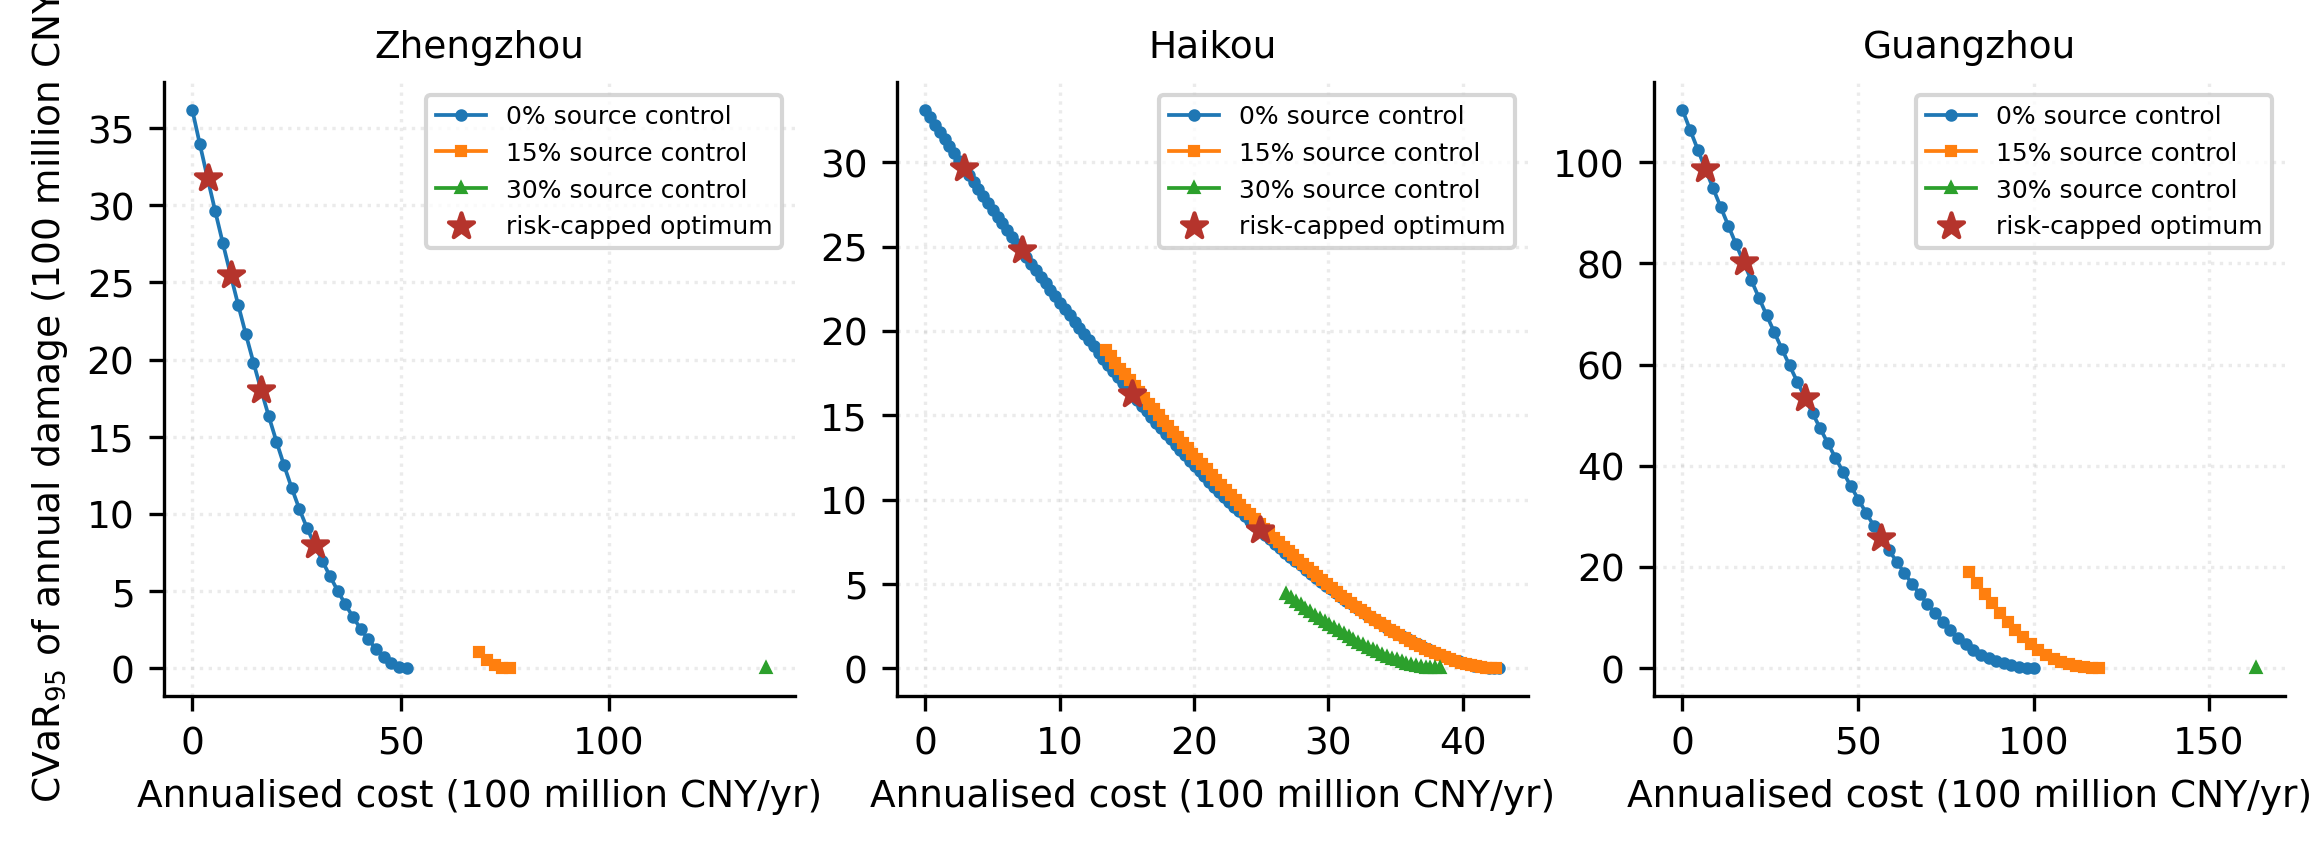
\includegraphics[width=0.36\linewidth]{../02_figures/fig23_q5_pareto.png}
\caption{Annualised cost against $\mathrm{CVaR}_{95}$ of annual damage for the three cities, for three source-control shares; stars mark the cost-minimal design under each risk cap. Lower-left is better and the frontier is the lower envelope.}
\label{fig:pareto}
\end{figure}

Three results follow. First, without a risk cap no city invests: the unconstrained optimum is the status quo everywhere, the same verdict as the uniform menu. Second, a binding cap forces spending, and what it buys differs by city: at 90\%, 50\% and 25\% of baseline risk Zhengzhou buys 5, 22.5 and 40\,mm of storage (ratios 0.10, 0.085, 0.068), Guangzhou 7.5, 40 and 65\,mm of extra conveyance (0.27, 0.21, 0.17), and Haikou 20, 107.5 and 150\,mm of storage (0.17, 0.13, 0.11), the tightest cap adding 22.5\,mm of conveyance, i.e.\ a three-year equivalent standard, rather than source control. Third, every ratio here is below one while every hotspot ratio above is above one: \emph{a risk cap is a constraint, not an investment}. A city that must meet a residual-risk target should meet it at least cost, and the least-cost instrument is the hotspot, which this programme cannot buy because its decision variable is a city-wide depth.

\subsection{A three-speed construction plan}

\textbf{Speed 1: protect the hotspots (0--5 years).} Identify the 2--5\% of each city where damage density is at least ten times the average (underpasses, metro portals, underground car parks, hospitals, power substations) and protect exactly those with local storage, raised entrances, sealed shafts and pumped drainage. The ratio is 1.0--4.1 across the assumed pairs, the measure is reversible and fast, and closure protocols for underground space should be written into the operating licence, because the Zhengzhou failure was as much a decision failure as an engineering one.

\textbf{Speed 2: source control where it is cheap (5--15 years).} Green roofs, permeable pavement and detention ponds reduce the curve number and the runoff volume, at 150 million CNY per km$^2$ of full coverage. Our grid shows that 15--30\% coverage never pays on its own; it also delivers amenity and heat benefits the model does not monetise, so it belongs where land is cheap and redevelopment is already happening.

\textbf{Speed 3: conveyance capacity only where exposure is extreme (15--30 years).} Deep tunnels and large pumping stations cost a billion CNY per millimetre of design depth over a city like Zhengzhou; they pay only under a binding risk cap, and even there storage is the cheaper instrument. For most cities the money is better spent on the first two speeds plus non-structural measures.

\textbf{Cross-cutting: measure the right variable.} Section~\ref{sec:q3} showed that a daily-index screen misses a Zhengzhou-type disaster entirely. Every city should therefore archive sub-hourly precipitation and publish design storms at both a three-day and an hourly duration. The current Chinese standard (GB\,50014-2021 \cite{gb50014}, with GB\,55027-2022 \cite{gb55027}) already defines the storm-water system as source reduction, conveyance and detention plus non-structural measures, and sets design return periods of 1--3 years for ordinary, 3--5 for important and 10 for especially important areas; our results say that this ladder is reasonable for conveyance, but that the binding constraint on catastrophic loss is the unprotected hotspot, not the pipe diameter.

\textbf{Staged budget.} For Guangzhou, protecting 2\% of the 1\,400\,km$^2$ area with 5\,mm of local storage means $1.4\times10^{5}$\,m$^3$, about 112 million CNY at the unit cost used here; with sealed entrances and operating procedures the first phase stays well below half a billion CNY, several times less than one millimetre of city-wide capacity over the same area (1.19 billion CNY), and it returns 4.05 times its cost in avoided damage before deaths are counted.

\section{Sensitivity, strengths and weaknesses, conclusions}\label{sec:eval}

\subsection{Sensitivity analysis}

A result that flips under a plausible change of a nuisance parameter is not a result. Table~\ref{tab:params} in Appendix~\ref{app:params} records, for every parameter, whether it is assumed, estimated or calibrated, where it comes from, and whether it was swept; we report here what the sweeps changed.

\textbf{Curve number.} The capacity ratio of 5.6 is the observed peak hour divided by the design intensity and is therefore independent of CN by construction; it cannot be used as evidence of robustness. What does depend on CN is the volume. Runoff from the three-day event ranges from 2.72 to $3.52\times10^{8}$\,m$^3$ across CN\,75--95, and the time needed to drain that runoff at 36\,mm\,h$^{-1}$ from 6.4 to 8.3\,h, so the statement that the network was overloaded for most of a working day survives the whole bracket. In Task~5 the same bracket moves Haikou's best uniform ratio from 0.155 (CN\,75) to 0.274 (CN\,95): the level moves, the verdict does not.

\textbf{Shape parameter and estimation method.} Zhengzhou's tail is not identified, and the windows we use do not even agree on its sign, so every window is named. On the 1961--2020 daily maxima the MLE gives $\xi=-0.026$ and the L-moment fit $-0.001$; on 1961--2024, $-0.007$ and $+0.030$; on the 1961--2010 training window of Task~3, $-0.042$ and $-0.022$. The spread between estimators inside one window is as large as the spread between windows, which is the honest summary of a 50--60 year record. The 100-year level is therefore quoted as [139.2, 242.5]\,mm, and the 449\,mm total only as an order of magnitude ($1.6\times10^{8}$\,yr, interval 678\,yr to infinity), never as a number a planner should use. The estimator moves the Task~5 design depth by 0.5\% (102.9\,mm by L-moments against 102.4\,mm by MLE on 1961--2020) and Haikou's ratio from 0.181 to 0.179, so no conclusion rests on it.

\textbf{Prediction target.} The most influential choice in Task~3 is the predictand. Quantile versus expected maximum shifts RMSE by 9.1\,mm with a paired bootstrap interval of [3.3, 13.6]\,mm and bias by 21\,mm, more than any distributional assumption; the gain of the trend correction over the stationary expected maximum, 1.7\,mm with interval $[-1.9, 7.0]$, is inside the noise. Both targets are reported and the expected maximum is recommended for planning.

\textbf{Storm-type thresholds.} The type test uses a rarity ratio of 3 and a concentration gap of 0.10, while the observed values are 14.1 and 0.134. Relaxing the thresholds to 10 and 0.05 leaves both criteria violated, so the ``different type'' verdict is robust to the threshold choice.

\textbf{Investment parameters.} The damage exponent and the discount rate drive the Task~5 levels. Varying $\gamma$ over 1.2--1.8 and the discount rate over 2--6\% moves the best uniform ratio into 0.06--0.44 for all three cities (Guangzhou highest, Zhengzhou lowest), so no parameter combination on that range brings uniform capacity to break-even. Using MLE rather than L-moments for the two-year design depth moves the ratio by less than 0.003, so the tail estimator is not what drives the verdict. Anchoring the damage function on the station total (313.4\,mm) instead of the official areal 449\,mm rescales every ratio by 2.465, which lifts Guangzhou's hotspot ratio to 10.0 while leaving the uniform menu at or below 0.69 --- the hotspot conclusion is the robust one.

\subsection{Strengths}

{\small
\begin{itemize}[leftmargin=1.4em,itemsep=1pt,topsep=2pt]
\item \textbf{Reproducibility.} Every number is generated by the scripts in Appendix~\ref{app:code} from archived raw files with fixed seeds; the pipeline decodes both provider conventions and validates them against each other.
\item \textbf{Honest inference.} False-discovery control over one explicitly declared family of 146 tests, bootstrap intervals on the two comparisons that decide the paper, a heterogeneity test before any regional pooling, and an explicit refusal to interpret return periods beyond what the record supports.
\item \textbf{A real forecast experiment.} Task~3 is evaluated on held-out years with identical folds for ten methods, and the comparison identifies \emph{why} methods differ (target definition, bias, ranking) rather than only which wins.
\item \textbf{A decision-relevant result.} Hazard, exposure, vulnerability and cost share units, so the Task~5 policy follows from the Task~1--4 measurements; protecting 2\% of the area reaches 4.05 at a fraction of the cost of a uniform upgrade that reaches 0.28.
\end{itemize}}

\subsection{Weaknesses and how they would be fixed}

{\small
\begin{itemize}[leftmargin=1.4em,itemsep=1pt,topsep=2pt]
\item \textbf{Daily resolution.} The archives are daily, so the hourly peak enters only through the official record; this is why the daily screen ranks Zhengzhou low rather than first. Sub-hourly telemetry would fix it.
\item \textbf{Decomposition is an identity.} The three factors in Task~4 exhaust the loss gap by construction and do not establish causation; only the exposure mechanism is corroborated externally.
\item \textbf{Short held-out window.} The 300-valid-day rule leaves 5--7 test years per city, so RMSE carries a large sampling error and close calls (GEV versus Gumbel) should not be over-read.
\item \textbf{Loss granularity and hydraulics.} Losses are provincial and municipal rather than district-level, and the damage function is calibrated on one event; we compute volumes and capacity ratios, not street depths. A district inventory over several events plus a coupled 1D--2D model would let the exponent be estimated rather than assumed.
\item \textbf{Stationarity.} The hazard model is stationary with an optional linear trend and uses no climate projections; defensible for the baseline given the weak national trends, but a 30-year horizon should carry a scenario range, since observed intensification of sub-daily extremes \cite{ipcc2021} points the same way as our Zhengzhou result.
\end{itemize}}

\subsection{Conclusions}

\textbf{Task 1.} Zhengzhou's rainfall is not increasing in total; it is becoming more concentrated. Wet days fall by 2.0 per decade ($p=0.021$) while daily intensity rises, and no change point is detectable. The July 2021 daily total (188.7\,mm) was a 54-year empirical event and did not break the 1978 record, but the three-day total (313.4\,mm) was the largest in 71 years and the official 449\,mm lies beyond reliable extrapolation. The waterlogging was a capacity failure in time: the peak hour exceeded the one-year design intensity 5.6-fold, leaving $1.4\times10^{8}$\,m$^3$ above capacity, and the three-day runoff needed 7.4\,h to drain.

\textbf{Task 2.} Across 25 cities only 2 annual-total and 1 one-day-extreme trend survive false-discovery control, against 7 intensity and 9 wet-day trends: redistribution, not more rain. Six belts differ in the sign of the total trend (South $+21.5$, Southwest $-27.1$\,mm per decade) while every belt loses wet days, and two clusters capture the split (silhouette 0.336).

\textbf{Task 3.} The predictand matters more than the distribution: forecasting the expected maximum of $n$ years rather than the $T$-year quantile cuts RMSE from 64.8 to 55.7\,mm and bias from $-41.5$ to $-20.5$\,mm. Extreme-value models dominate machine learning on ranking (top-five overlap 4/5 versus 3/5 at best; Spearman 0.75 versus 0.64), while regression removes the bias. Five cities broke their record in the held-out window, none in 2021, which exposes the blind spot of daily indices for sub-daily disasters. Fuzhou, Haikou, Guangzhou and Hohhot carry the highest ten-year exceedance probabilities; Zhengzhou ranks sixteenth on probability and tenth on the composite.

\textbf{Task 4.} The two storms are different types. Zhengzhou is an intensity-type event (1-day return period 134.5 years, 52\% of the event total in one day, 201.9\,mm in one hour); Taiyuan is a persistence-type event (9.5-year return period, concentration at the 6.5th percentile of its own climatology). Losses differ by 23.9, of which 1.07 is the area ratio; the remaining 22.4 splits into population density (2.68), affected share (2.95) and loss per affected person (2.84), and a Shapley decomposition assigns $31.3$, $33.6$ and $32.7\%$ to the three, so removing any one still leaves 8.1--8.9. Rainfall depth differs by only 2.2, so the gap is exposure and vulnerability, not meteorology. Zhengzhou should be screened on hourly intensity, Taiyuan on multi-day accumulation.

\textbf{Task 5.} Uniform capacity is never the efficient first purchase once damage is priced per unit of overflow volume: across the 378-point menu the best ratio is 0.28 (Guangzhou), 0.18 (Haikou) and 0.10 (Zhengzhou), and no social plan exceeds 0.26. Protecting the 2\% most exposed area, where damage density is twenty times the average, yields 4.05, 2.62 and 1.50 for the same money --- the reverse of the hazard ordering, because absolute damage density decides whether a hotspot investment pays. Under a CVaR$_{95}$ cap no city invests without one and every cap is met below 0.28, so a cap is a constraint to satisfy at least cost, and the least-cost instrument is the hotspot. The plan is therefore three-speed: hotspots and closure protocols within five years, source control where redevelopment makes it cheap within fifteen, and large conveyance only where exposure is extreme. Because a daily screen cannot see a Zhengzhou-type event, every city should archive sub-hourly rainfall.

\newpage
\begin{thebibliography}{99}
\addcontentsline{toc}{section}{References}

\bibitem{sc} State Council Disaster Investigation Group. \emph{Investigation Report on the ``7.20'' Extreme Rainstorm Disaster in Zhengzhou, Henan}. Beijing, January 2022. \url{https://www.mem.gov.cn/gk/sgcc/tbzdsgdcbg/202201/P020220121639049697767.pdf} (accessed 17 November 2026).

\bibitem{che2021} Che S., Li X., Ding T., Gao H. Autumn behaving like summer: analysis of the persistent damaging rainstorm and water-vapour extremes in northern China in early October 2021. \emph{Transactions of Atmospheric Sciences}, 44(6): 825--834, 2021. DOI 10.13878/j.cnki.dqkxxb.20211029001.

\bibitem{mem2021} Ministry of Emergency Management of China. \emph{National Natural Disasters in October 2021}. Beijing, November 2021. \url{https://www.mem.gov.cn/xw/yjglbgzdt/202111/t20211102_401401.shtml} (accessed 17 November 2026).

\bibitem{pettitt1979} Pettitt A.N. A non-parametric approach to the change-point problem. \emph{Applied Statistics}, 28(2): 126--135, 1979.

\bibitem{menne2012} Menne M.J., Durre I., Vose R.S., Gleason B.E., Houston T.G. An overview of the Global Historical Climatology Network-Daily database. \emph{Journal of Atmospheric and Oceanic Technology}, 29(7): 897--910, 2012.

\bibitem{sen1968} Sen P.K. Estimates of the regression coefficient based on Kendall's tau. \emph{Journal of the American Statistical Association}, 63(324): 1379--1389, 1968.

\bibitem{mann1945} Mann H.B. Nonparametric tests against trend. \emph{Econometrica}, 13(3): 245--259, 1945.

\bibitem{coles2001} Coles S. \emph{An Introduction to Statistical Modeling of Extreme Values}. London: Springer, 2001.

\bibitem{neh1986} United States Department of Agriculture, Soil Conservation Service. \emph{Urban Hydrology for Small Watersheds}, Technical Release 55. Washington DC, 1986.

\bibitem{bh1995} Benjamini Y., Hochberg Y. Controlling the false discovery rate: a practical and powerful approach to multiple testing. \emph{Journal of the Royal Statistical Society B}, 57(1): 289--300, 1995.

\bibitem{hosking1985} Hosking J.R.M., Wallis J.R., Wood E.F. Estimation of the generalized extreme-value distribution by the method of probability-weighted moments. \emph{Technometrics}, 27(3): 251--261, 1985.

\bibitem{hosking1997} Hosking J.R.M., Wallis J.R. \emph{Regional Frequency Analysis: An Approach Based on L-Moments}. Cambridge University Press, 1997.

\bibitem{hosking1993} Hosking J.R.M., Wallis J.R. Some statistics useful in regional frequency analysis. \emph{Water Resources Research}, 29(2): 271--281, 1993.

\bibitem{gb50014} Ministry of Housing and Urban-Rural Development of China. \emph{GB 50014-2021 Code for Design of Outdoor Wastewater Engineering}. Beijing: China Planning Press, 2021.

\bibitem{gb55027} Ministry of Housing and Urban-Rural Development of China. \emph{GB 55027-2022 General Code for Urban Drainage and Waterlogging Prevention}. Beijing, 2022.

\bibitem{ipcc2021} IPCC. \emph{Climate Change 2021: The Physical Science Basis}. Contribution of Working Group I to the Sixth Assessment Report, Chapter 8 (Water Cycle Changes) and Chapter 11 (Weather and Climate Extremes). Cambridge University Press, 2021.

\end{thebibliography}

\newpage
\appendix
\section{Notation}\label{app:notation}

\begin{table}[H]
\centering
\caption{Principal symbols.}
\label{tab:notation}
\small
\begin{tabular}{ll}
\toprule
Symbol & Meaning\\
\midrule
$P_d$ & daily precipitation (mm)\\
$\mathrm{Rx1day}$, $\mathrm{Rx5day}$ & annual maximum 1-day and 5-day rainfall (mm)\\
$\mathrm{SDII}$ & simple daily intensity index (mm per wet day)\\
$\mathrm{R95p}$, $\mathrm{R99p}$ & annual total of days above the 95th/99th wet-day percentile (mm)\\
$\beta$, $p$ & Sen slope per decade and Mann--Kendall $p$-value\\
$q$ & Benjamini--Hochberg adjusted $p$-value\\
$\mu,\sigma,\xi$ & GEV location, scale and shape parameters\\
$\mathrm{RL}(T)$ & return level for return period $T$ (years)\\
$M_n$ & maximum of $n$ future annual maxima\\
$\mathbb{E}[M_n]$ & expected maximum, $\int_0^1F^{-1}(u^{1/n})du$\\
$\mathrm{CN}$ & SCS curve number\\
$S_{\text{ret}}$ & potential maximum retention, $25400/\mathrm{CN}-254$ (mm)\\
$Q$ & runoff depth (mm)\\
$C$ & design capacity, $\mathrm{RL}_{3d}(T)+S_{\text{sto}}$ (mm)\\
$O$ & overflow, $(Q(X)-C)^+$ (mm), where $Q(X)$ is the SCS runoff of event rainfall $X$\\
$S_{\text{sto}}$, $T$ & distributed storage depth (mm) and design return period (years)\\
$D$ & damage (CNY)\\
$h$, $m$ & protected area fraction and hotspot damage multiplier\\
$g$ & green source-control coverage fraction\\
$\mathrm{BCR}$ & benefit--cost ratio\\
$\mathrm{CVaR}_{95}$ & conditional value-at-risk at the 95\% level\\
\bottomrule
\end{tabular}
\end{table}

\section{Parameter provenance}\label{app:params}

\begin{table}[H]
\centering
\caption{Every parameter of the study: status (A assumed, E estimated, C calibrated), value, source, and whether it was swept in Section~\ref{sec:eval}.}
\label{tab:params}
\footnotesize
\setlength{\tabcolsep}{4pt}
\begin{tabular}{@{}p{0.30\linewidth}p{0.08\linewidth}p{0.15\linewidth}p{0.31\linewidth}p{0.06\linewidth}@{}}
\toprule
Parameter & Status & Value & Source & Swept\\
\midrule
Valid-day threshold & A & 300 d & data-quality choice; 4 of the 30 stations with data fall below 45 valid years & no\\
Study area, Zhengzhou & C & 1\,180\,km$^2$ & municipal administrative area & no\\
Curve number & A & 85 & TR-55 class C soil, 70\% impervious & 75--95\\
Design intensity & A & 36/43/50 mm h$^{-1}$ & GB 50014-2021, 1/2/3-year return period & 36--50\\
Rainfall normal 640.8 mm & C & 640.8 mm & Problem B statement & --\\
Damage exponent $\gamma$ & A & 1.5 & convexity of urban flood damage & 1.2--1.8\\
Reference overflow $O_{\text{ref}}$ & C & 296.4 mm & $Q(449)-RL_{3d}(2)=399.4-102.9$; the station-scale analogue uses $O=Q(313.4)-RL_{3d}(2)=265.4-102.9=162.4$ mm & 2.465$\times$\\
Pipe unit cost & A & $10^{9}$ CNY mm$^{-1}$ & planning-grade order of magnitude & grid\\
Storage unit cost & A & 800 CNY m$^{-3}$ & planning-grade; Happy Valley 1\,800 & 400--1\,600\\
Source-control cost & A & $1.5\times10^{8}$ CNY km$^{-2}$ & sponge-city range 1.0--1.8 & 15--30\% coverage\\
Curve-number credit & A & 40 units at 30\% coverage & literature range 20--50 & 0--40\\
Value of a statistical life & A & $5\times10^{6}$ CNY & Chinese road-safety studies & $1$--$15\times10^{6}$\\
Death elasticity & A & 1.5 & assumed & no\\
Discount rate & A & 4\% & planning practice & 2--6\%\\
O\&M and renewal & A & 2\% yr$^{-1}$ & planning practice & no\\
Risk aversion on CVaR$_{95}$ & A & 0.5 & assumed & 0--1\\
Hotspot fraction $h$, multiplier $m$ & A & 2--5\%, 10--20 & assumption of the protection experiment & both\\
\bottomrule
\end{tabular}
\end{table}

\section{Data appendix}\label{app:data}

\begin{longtable}{lrrrrr}
\caption{Stations of the national panel: latitude, longitude, valid years in 1961--2020, mean annual total and mean annual maximum one-day rainfall.}\label{tab:stations}\\
\toprule
City & Lat & Lon & Years & Total (mm) & Rx1day (mm)\\
\midrule
\endfirsthead
\toprule
City & Lat & Lon & Years & Total (mm) & Rx1day (mm)\\
\midrule
\endhead
\bottomrule
\endfoot
Beijing & 39.93 & 116.28 & 53 & 556 & 72.7 \\
Dalian & 38.90 & 121.63 & 53 & 628 & 91.6 \\
Hohhot & 40.82 & 111.68 & 53 & 399 & 53.3 \\
Jinan & 36.60 & 117.05 & 53 & 698 & 93.6 \\
Taiyuan & 37.78 & 112.55 & 53 & 447 & 56.1 \\
Yuncheng & 35.05 & 111.05 & 53 & 528 & 58.3 \\
Harbin & 45.75 & 126.77 & 53 & 528 & 56.1 \\
Shenyang & 41.73 & 123.52 & 53 & 692 & 74.6 \\
Lanzhou & 36.05 & 103.88 & 48 & 309 & 33.1 \\
Urumqi & 43.80 & 87.65 & 53 & 274 & 28.6 \\
Xining & 36.62 & 101.77 & 53 & 390 & 31.1 \\
Yinchuan & 38.47 & 106.20 & 53 & 192 & 34.9 \\
Fuzhou & 26.08 & 119.28 & 53 & 1371 & 103.9 \\
Guangzhou & 23.22 & 113.48 & 53 & 1752 & 124.6 \\
Haikou & 20.00 & 110.25 & 52 & 1688 & 165.9 \\
Nanning & 22.63 & 108.22 & 53 & 1293 & 104.9 \\
Guiyang & 26.58 & 106.73 & 53 & 1110 & 80.4 \\
Kunming & 25.02 & 102.68 & 53 & 994 & 75.0 \\
Hangzhou & 30.23 & 120.17 & 53 & 1402 & 89.9 \\
Hefei & 31.87 & 117.23 & 53 & 994 & 90.1 \\
Nanchang & 28.60 & 115.92 & 53 & 1594 & 115.8 \\
Nanjing & 31.93 & 118.90 & 53 & 1067 & 100.8 \\
Wuhan & 30.60 & 114.05 & 52 & 1247 & 118.9 \\
Xian & 34.30 & 108.93 & 48 & 562 & 51.4 \\
Zhengzhou & 34.72 & 113.65 & 53 & 642 & 82.7 \\
\end{longtable}


\section{Code appendix}\label{app:code}

All results are produced by the scripts below, run in order from \texttt{01\_code/} with the archived inputs. Seeds are fixed where randomness enters: 20210720 for every parametric bootstrap and Monte Carlo heterogeneity test, 0 for $k$-means, the random forest and the gradient-boosted trees. Two scripts read no random number at all (\texttt{s05\_q4.py}, \texttt{s09\_q4\_shapley.py}), so no seed applies to them; a rerun reproduces every table to the printed precision.

\begin{table}[H]
\centering
\caption{Reproducibility inventory. Scripts are listed in execution order.}
\footnotesize
\setlength{\tabcolsep}{4pt}
\begin{tabular}{@{}lp{0.66\linewidth}@{}}
\toprule
Script & Function\\
\midrule
\texttt{common.py} & I/O, unit decoding, annual indices, MK/Sen/Pettitt, GEV (MLE and L-moments), bootstrap\\
\texttt{s01\_prepare.py} & merge attachment and GHCN, quality control, cross-source validation\\
\texttt{s02\_q1.py} & Task 1 trends, change point, return levels, SCS-CN waterlogging budget\\
\texttt{s02b\_q1\_peak.py} & Task 1 peak-hour excess volume stored as an artefact\\
\texttt{s03\_q2.py} & Task 2 national panel, FDR control, clustering, regional aggregation\\
\texttt{s04\_q3.py} & Task 3 ten forecast strategies, record-breaker identification, risk ranking\\
\texttt{s04b\_q3\_risk\_table.py} & Task 3 single-definition ten-year exceedance probability for 23 cities\\
\texttt{s04c\_q3\_risk\_figs.py} & Task 3 risk map and ranking figure drawn from that table\\
\texttt{s05\_q4.py} & Task 4 event indices, type test, loss decomposition\\
\texttt{s06\_q5.py} & Task 5 GEV hazard, damage calibration, portfolio optimisation with CVaR\\
\texttt{s06b\_q5\_selective.py} & Task 5 targeted-protection variant\\
\texttt{s06c\_q5\_sensitivity.py} & Task 5 sweeps of $\gamma$, discount rate, CN, tail estimator, value of life\\
\texttt{s07\_q3\_regional.py} & Task 3 index-flood pooling, Hosking--Wallis heterogeneity test, grouped growth curves\\
\texttt{s08\_q5\_sp.py} & Task 5 risk-capped stochastic programme, cost--CVaR frontier\\
\texttt{s09\_q4\_shapley.py} & Task 4 Shapley decomposition of the loss gap, single-factor removal\\
\texttt{s10\_q5\_compare.py} & Task 5 uniform-versus-hotspot comparison figure and table\\
\bottomrule
\end{tabular}
\end{table}

Intermediate outputs are written as CSV and JSON under \texttt{03\_results/}; the figures of this paper are regenerated by the same scripts into \texttt{02\_figures/}. No number in the text is typed by hand: each is read from a JSON or CSV artefact, which is why the tables can be audited against the files.

\section{Additional figures}\label{app:extrafig}

\begin{figure}[H]
\centering
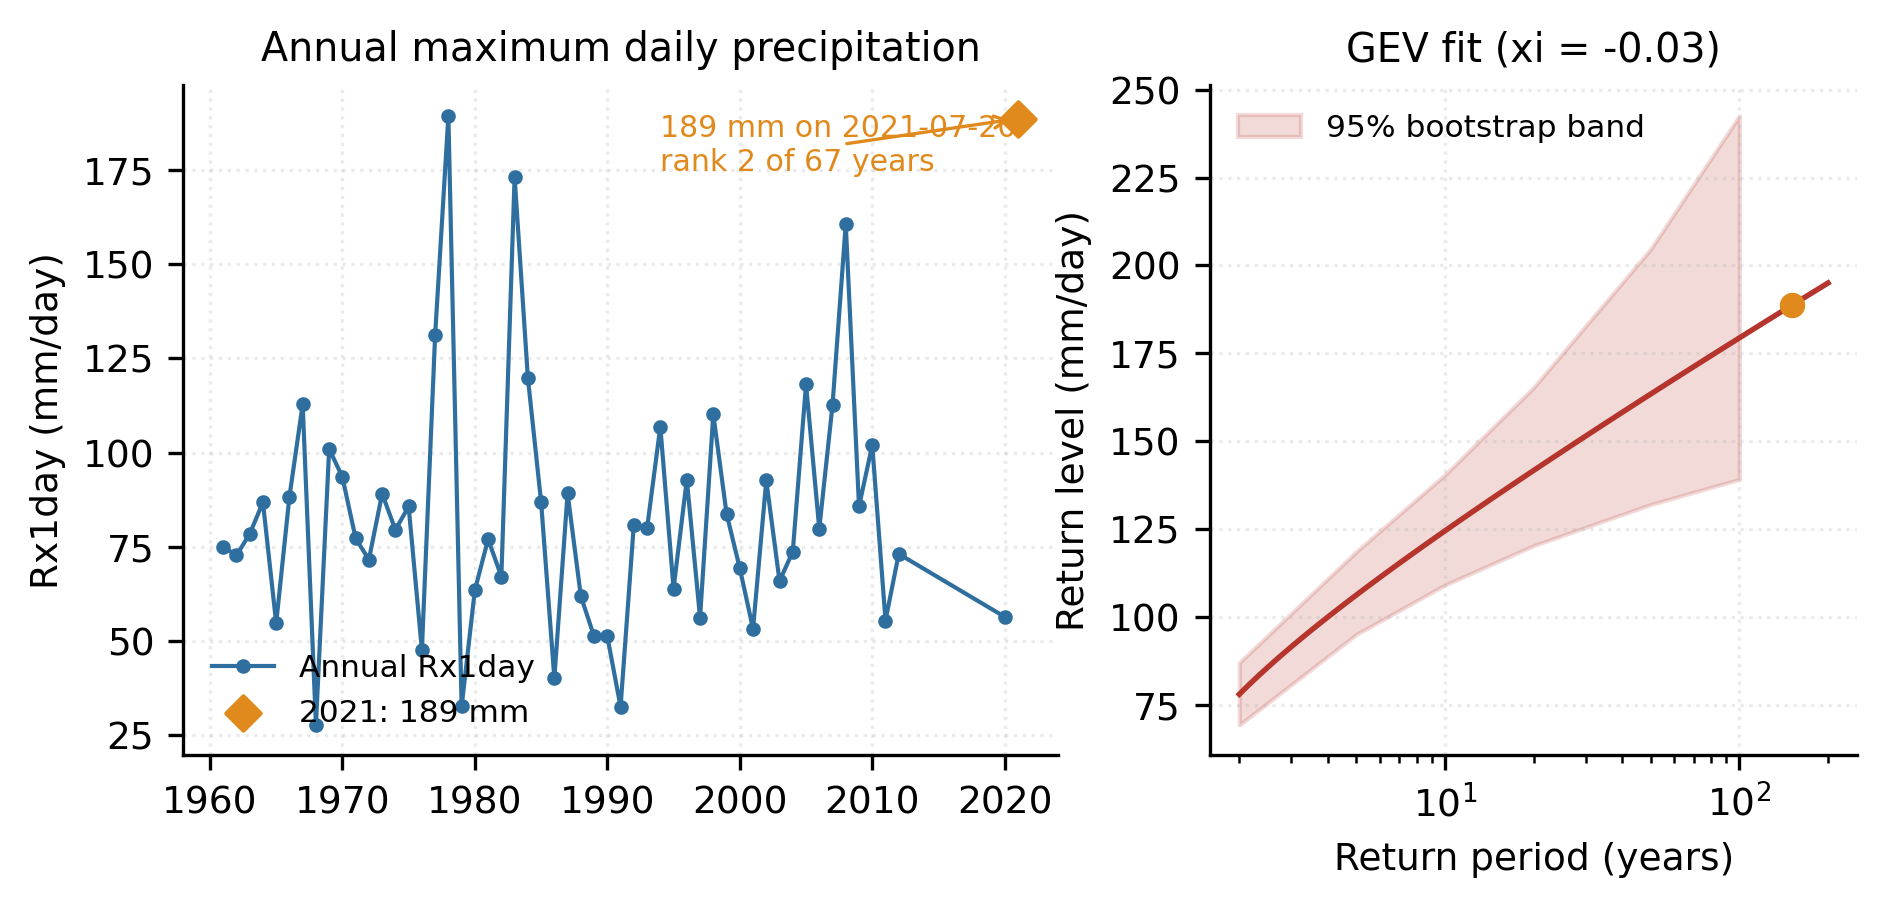
\includegraphics[width=0.62\linewidth]{../02_figures/fig02_rx1day_gev.png}
\caption{Annual maximum one-day rainfall at Zhengzhou with the fitted GEV curve; the 2021 value (188.7\,mm, marker) sits above the 100-year level of 179.4\,mm.}
\label{fig:rx1day}
\end{figure}

\begin{figure}[H]
\centering
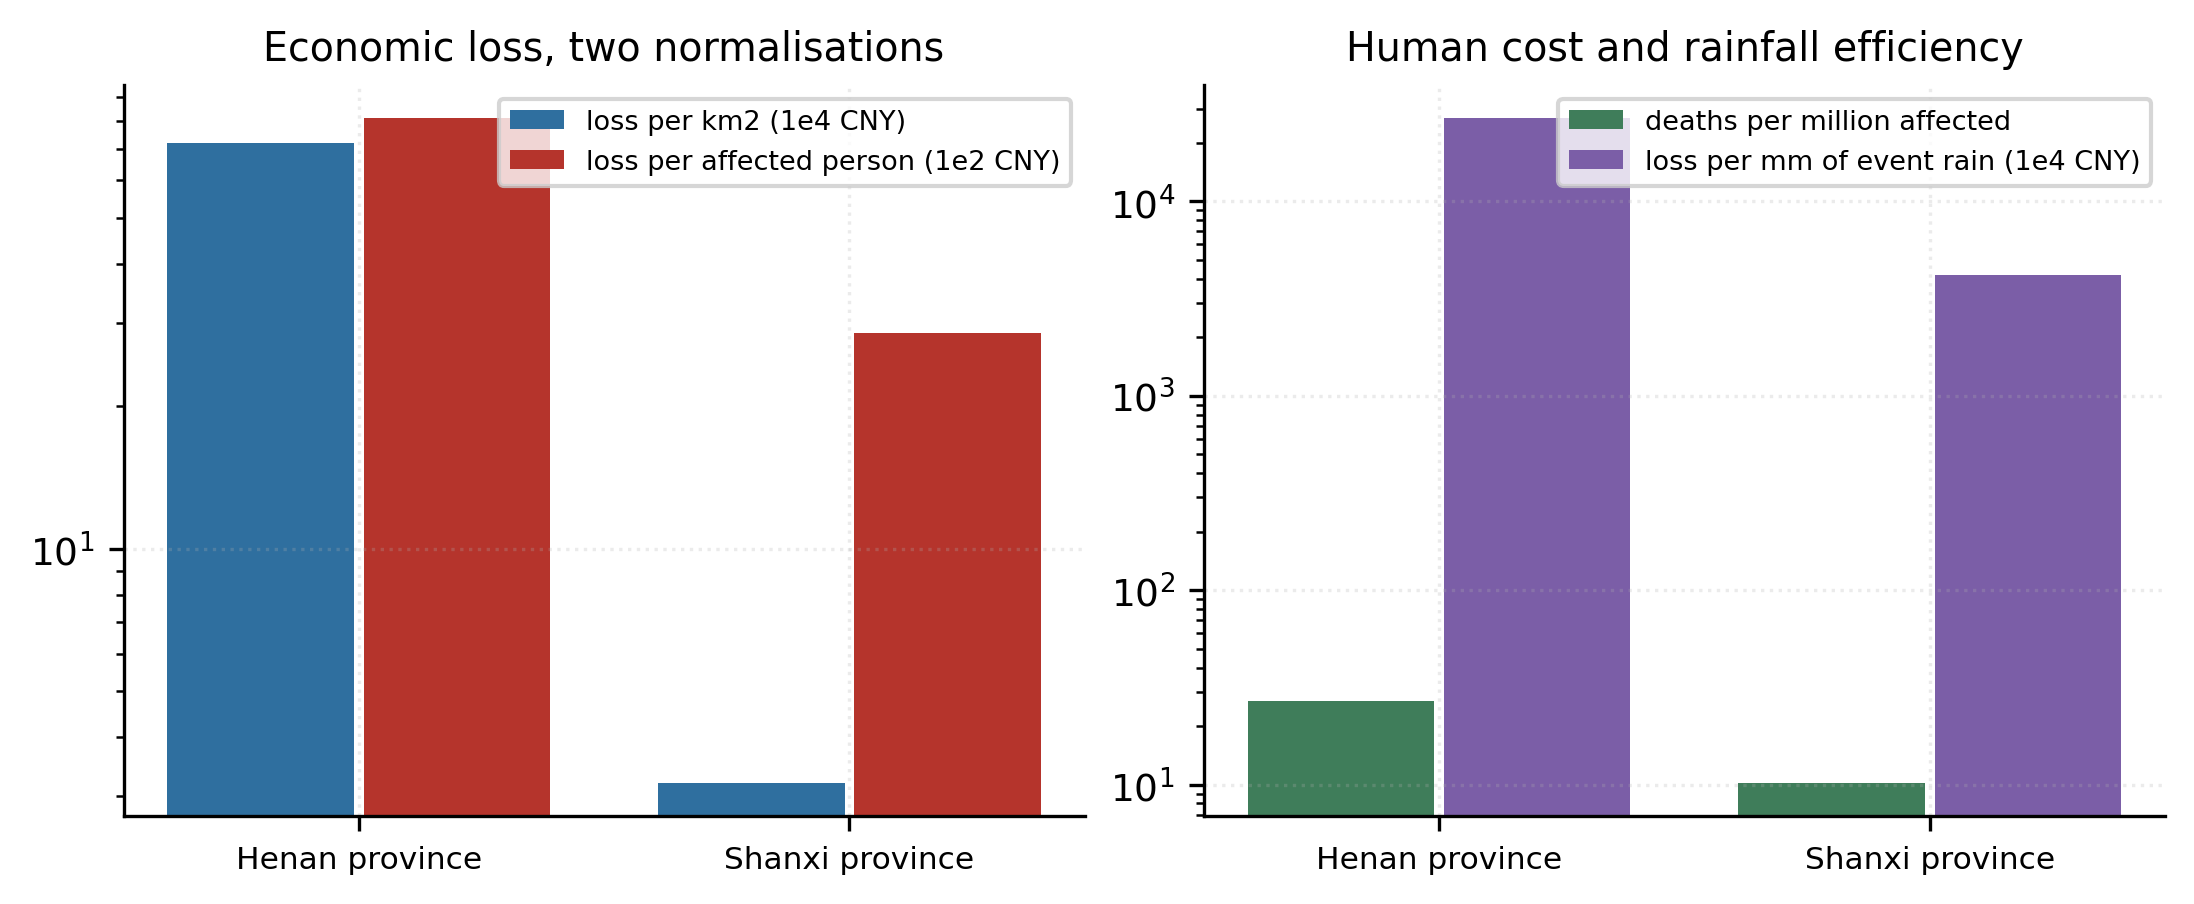
\includegraphics[width=0.62\linewidth]{../02_figures/fig19_loss_normalised.png}
\caption{Two normalisations of the loss. Left: loss per km$^2$ and loss per affected person. Right: deaths per million affected and loss per mm of event rainfall; the two rainfall denominators differ (the official 449\,mm areal total for Henan, a province-wide four-day mean for Shanxi), so that bar is indicative only.}
\label{fig:lossnorm}
\end{figure}

\begin{figure}[H]
\centering
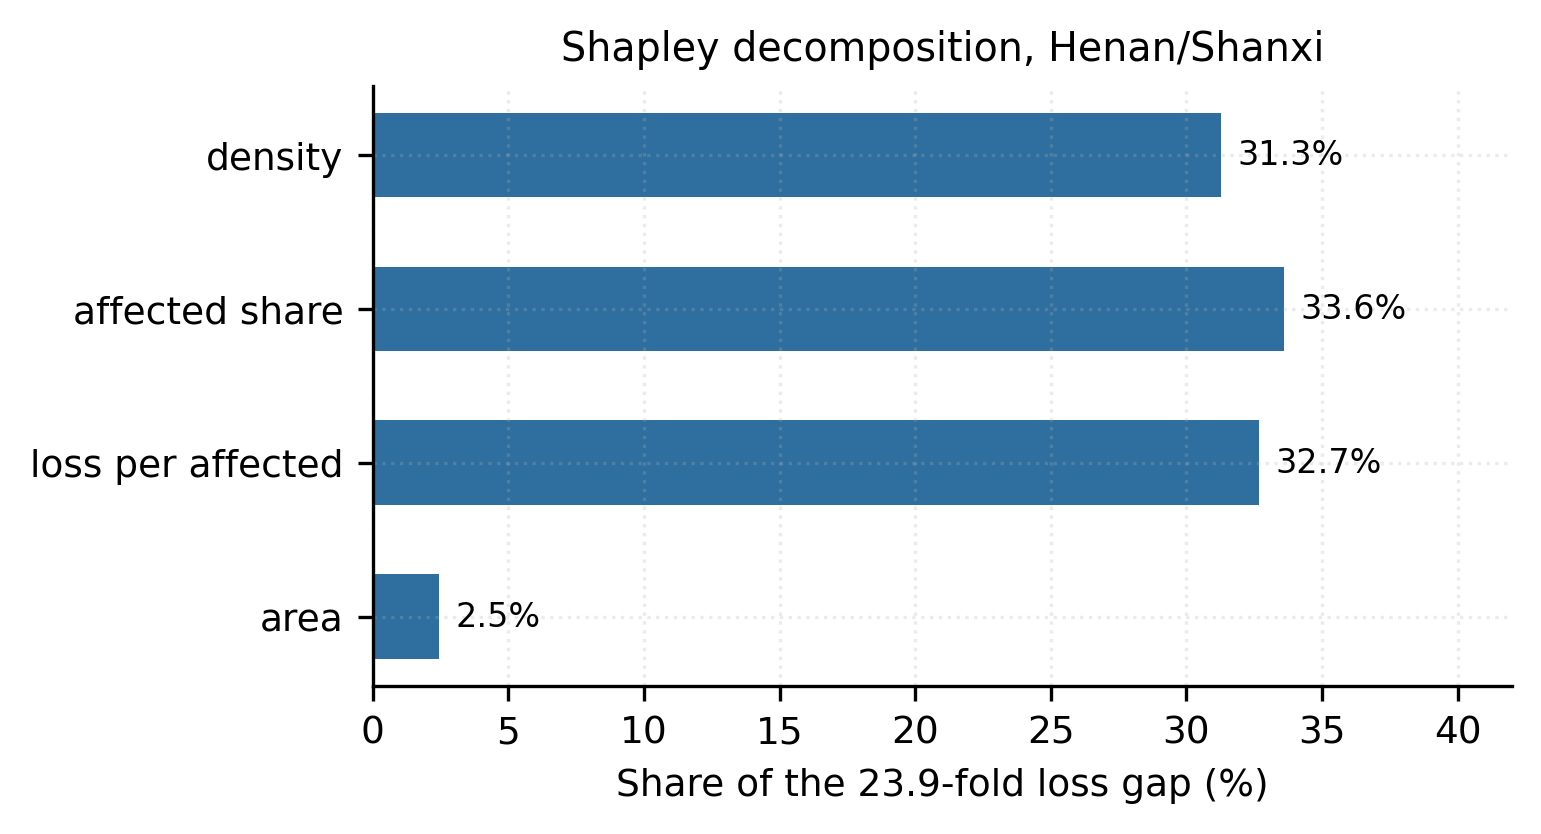
\includegraphics[width=0.58\linewidth]{../02_figures/fig24_q4_shapley.png}
\caption{Shapley shares of the 23.9-fold loss gap between Henan and Shanxi, with the four factors as players and partial products as coalition worth. Density, affected share and loss per affected person divide the gap almost equally; area contributes $2.5\%$.}
\label{fig:shapley}
\end{figure}

\begin{figure}[H]
\centering
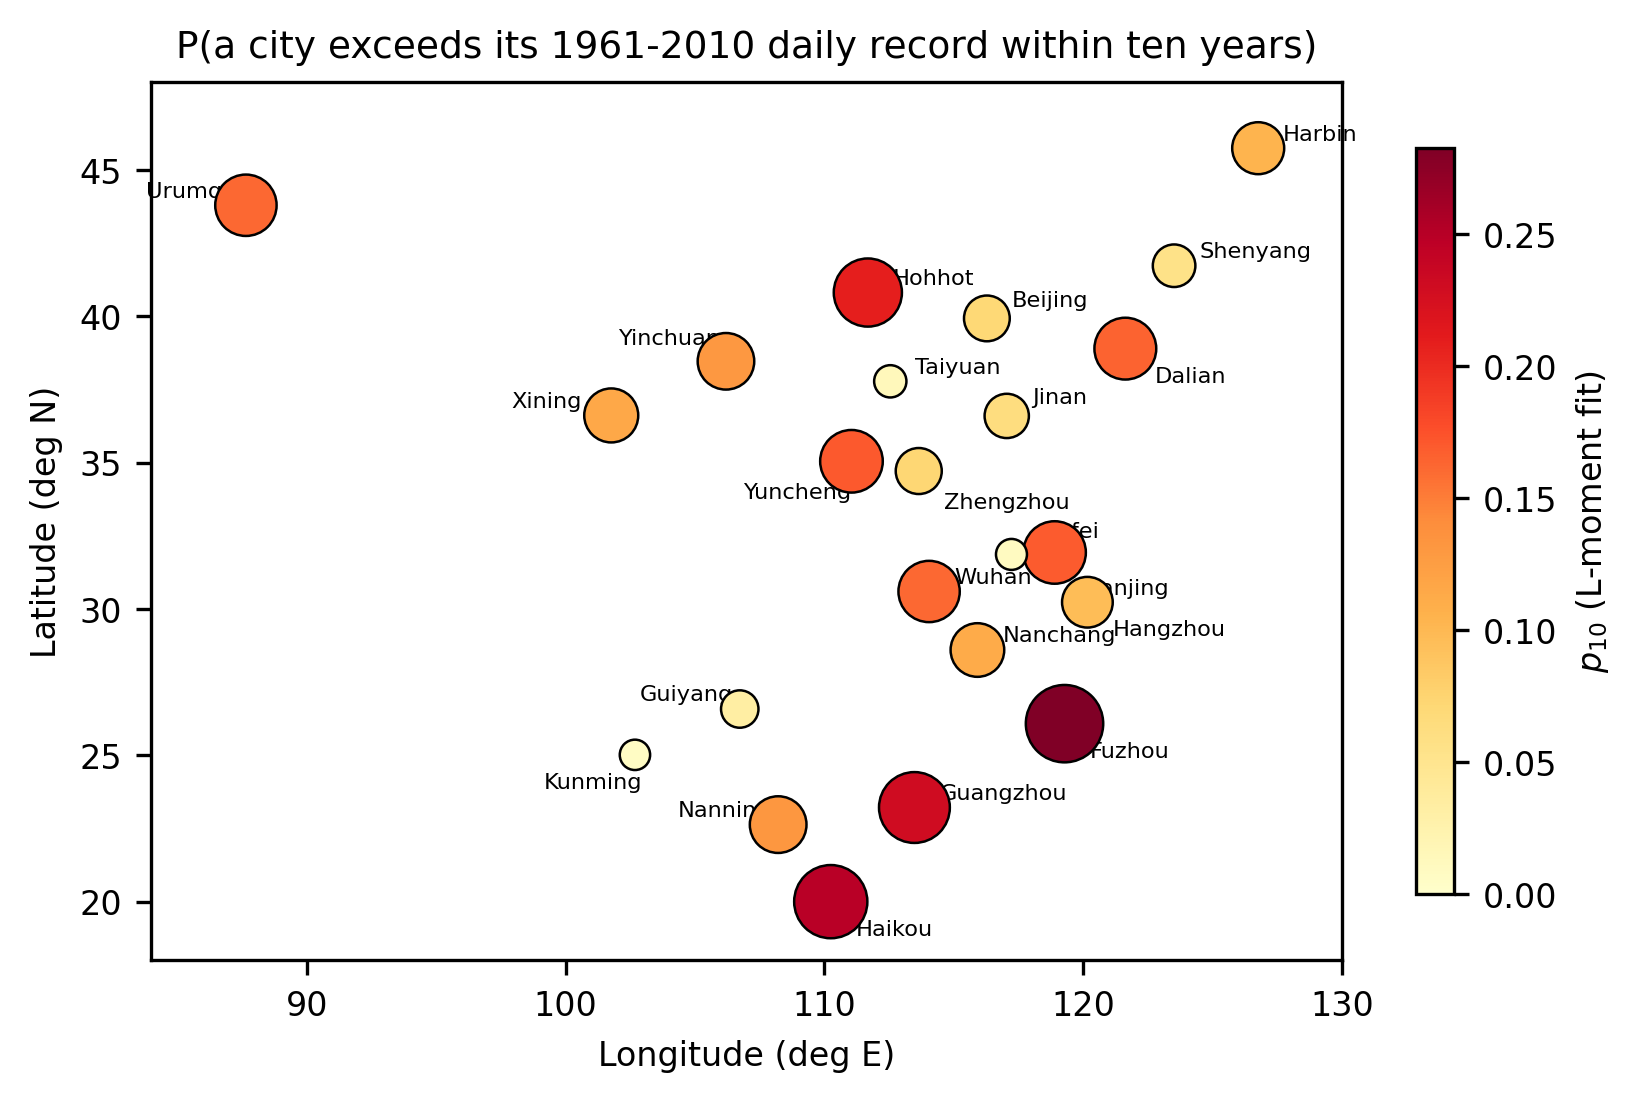
\includegraphics[width=0.62\linewidth]{../02_figures/fig14_risk_map.png}
\caption{Ten-year probability $p_{10}$ of exceeding the 1961--2010 daily record for the 23 cities, from the L-moment fit; the marker area is proportional to $p_{10}$.}
\label{fig:riskmap}
\end{figure}

\begin{figure}[H]
\centering
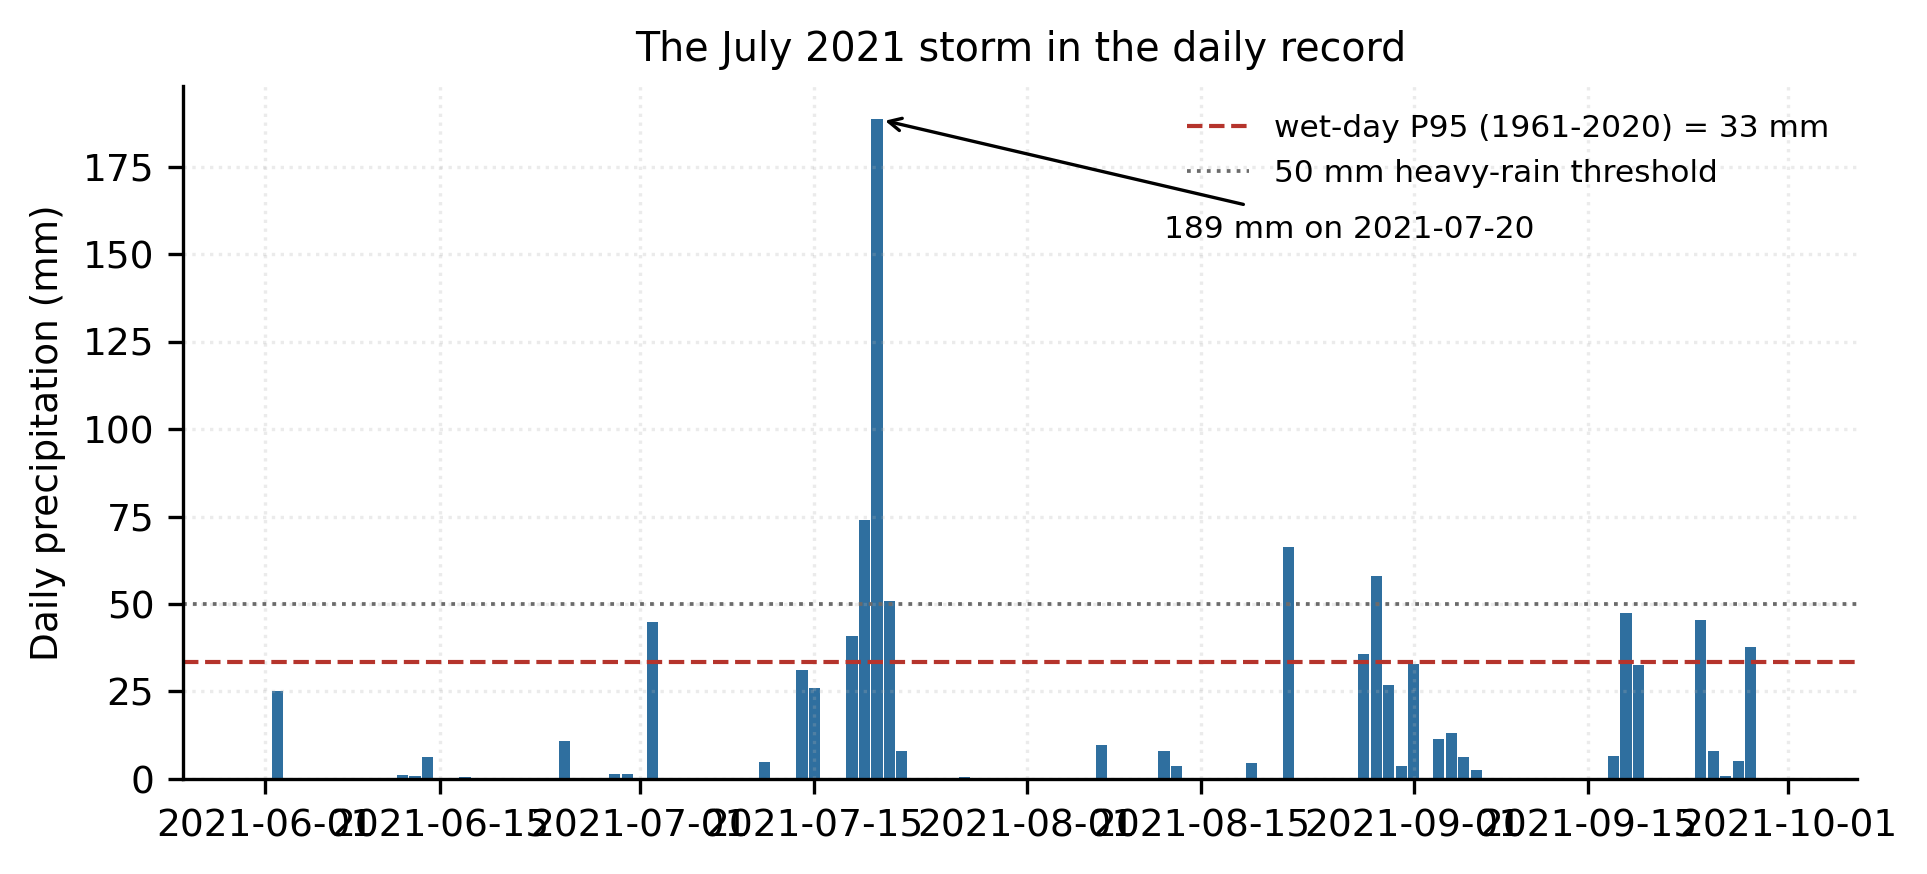
\includegraphics[width=0.62\linewidth]{../02_figures/fig05_event_profile.png}
\caption{The July 2021 storm in the daily record (1 June--30 September 2021). Dashed red line: wet-day 95th percentile of 1961--2020; dotted grey line: the 50\,mm heavy-rain threshold; the annotated bar is 188.7\,mm on 20 July.}
\label{fig:profile}
\end{figure}

\begin{figure}[H]
\centering
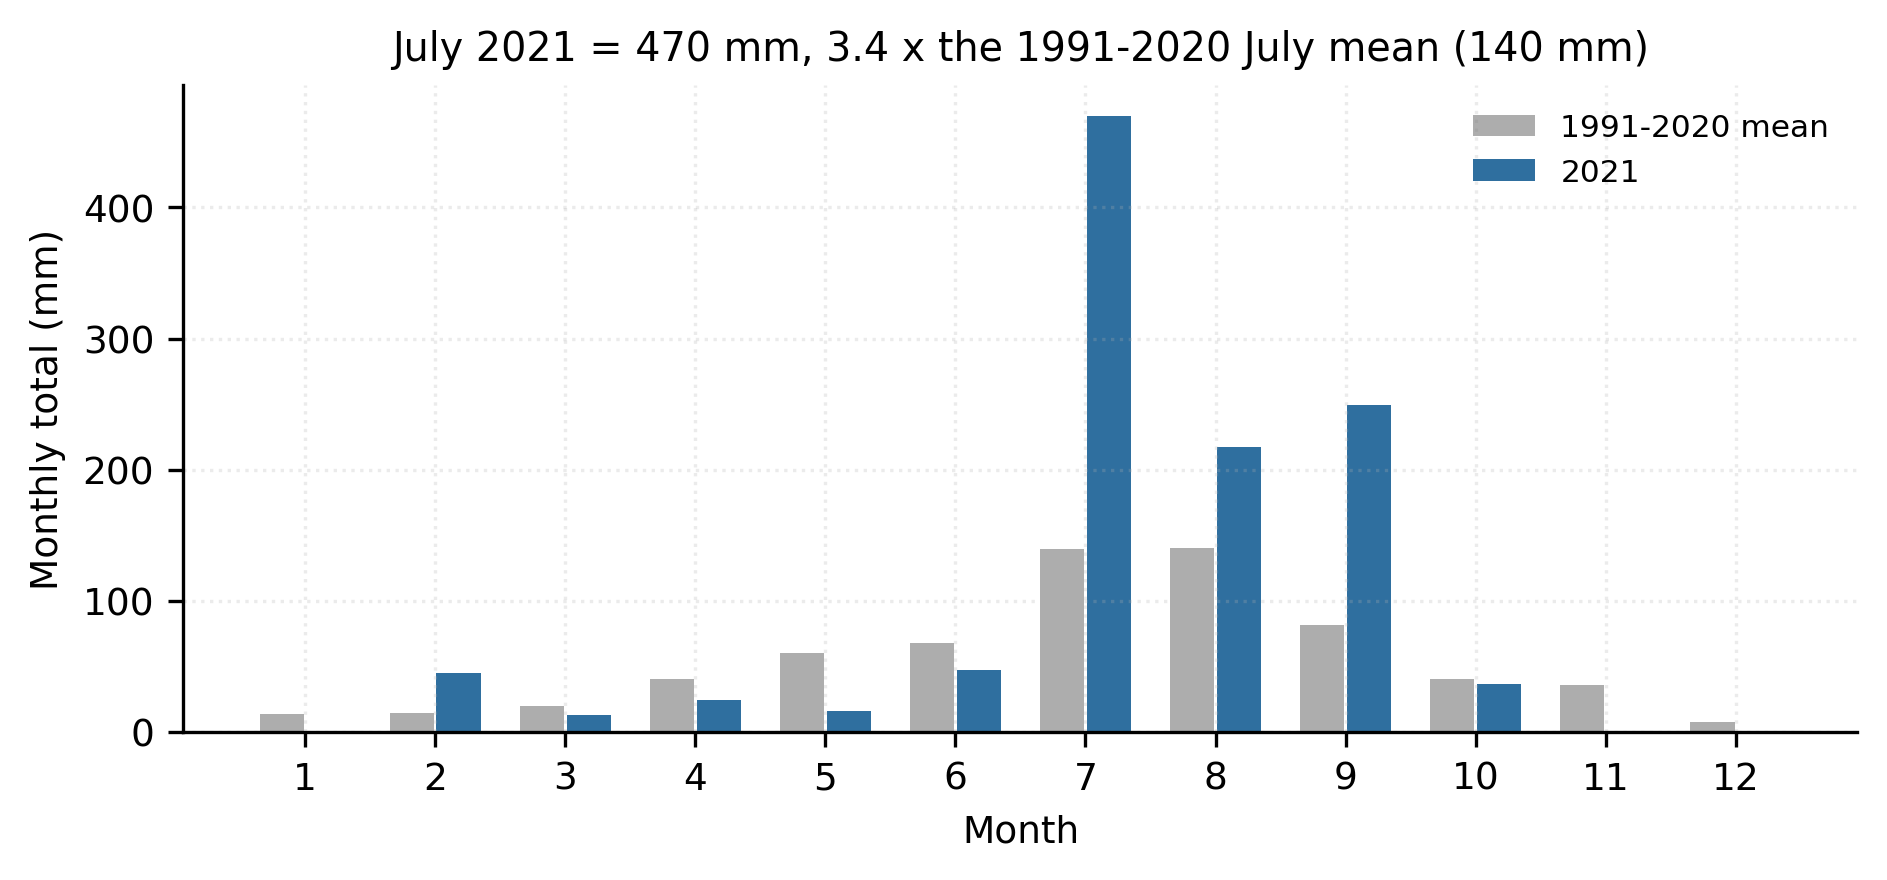
\includegraphics[width=0.62\linewidth]{../02_figures/fig03_monthly_2021.png}
\caption{Monthly totals in 2021 against the 1991--2020 monthly means. July 2021 reached 469.6\,mm, 3.4 times the July normal of 139.8\,mm.}
\end{figure}

\begin{figure}[H]
\centering
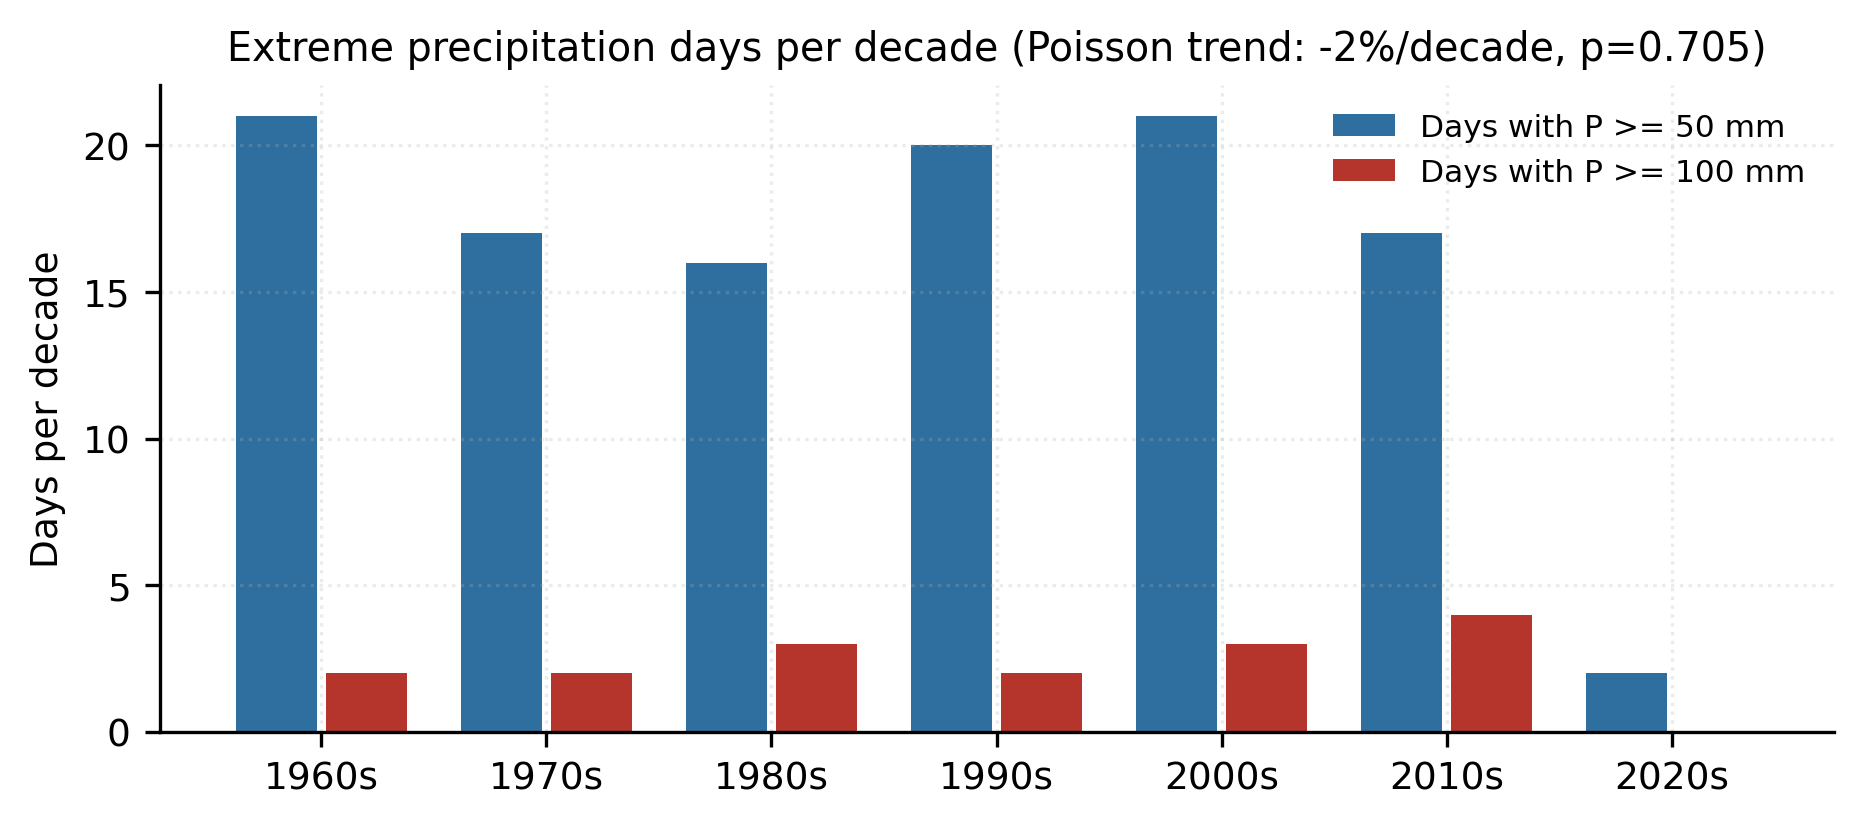
\includegraphics[width=0.62\linewidth]{../02_figures/fig04_extreme_days.png}
\caption{Decadal counts of days with precipitation above 50\,mm and above 100\,mm at Zhengzhou. The Poisson trend for days above 50\,mm is $-2.0\%$ per decade ($p=0.705$).}
\end{figure}

\begin{figure}[H]
\centering
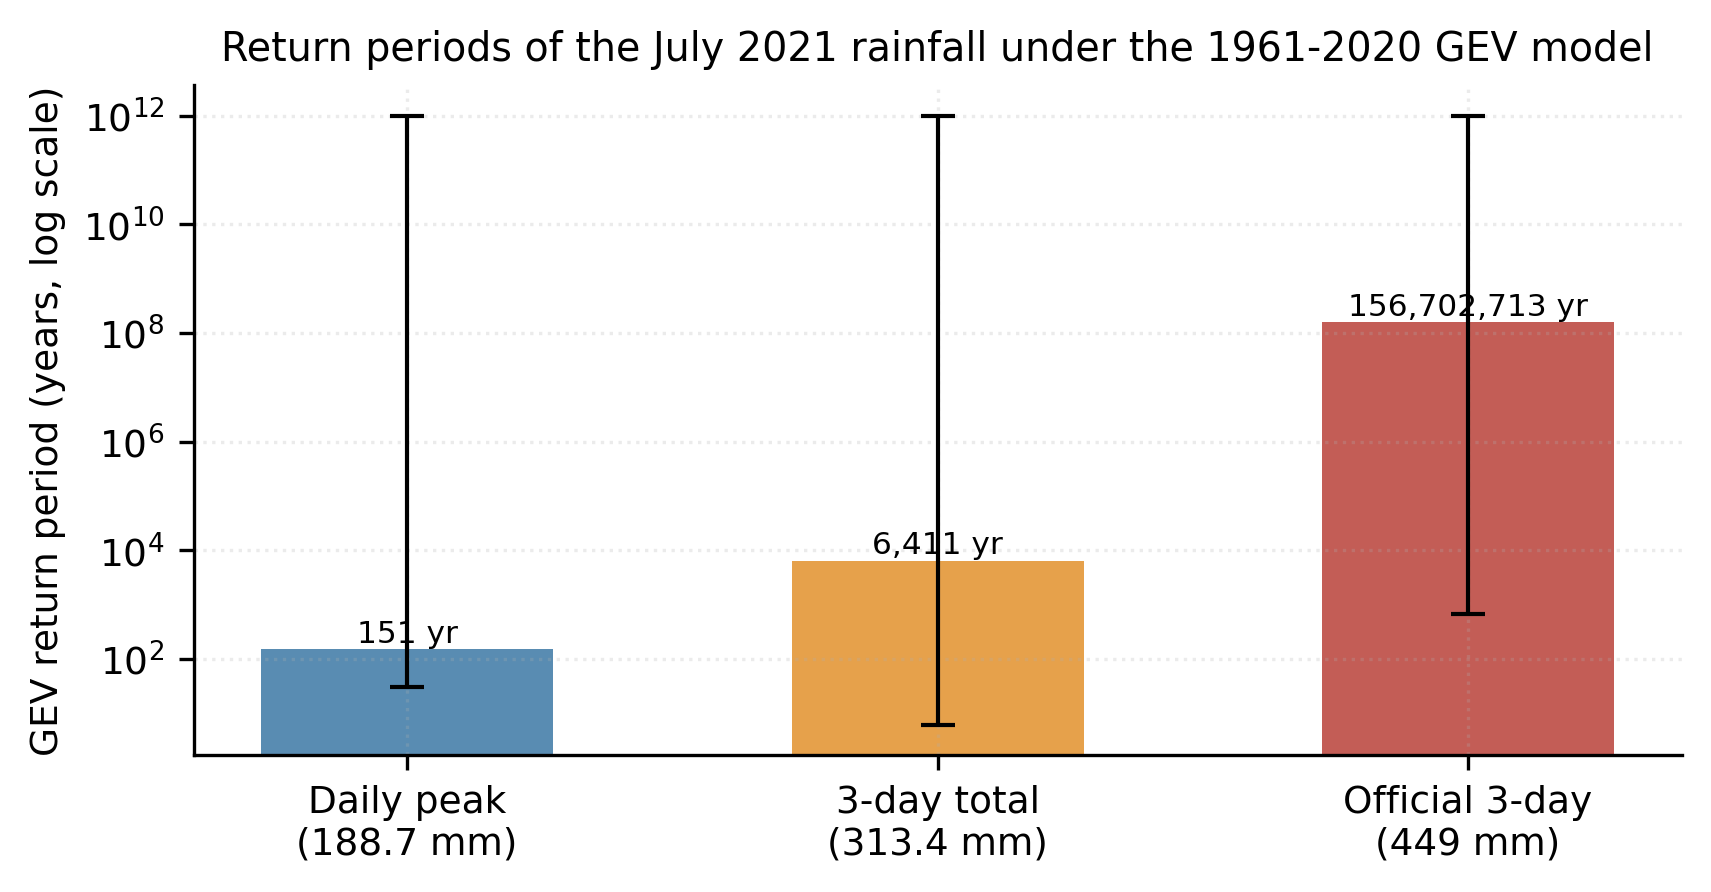
\includegraphics[width=0.58\linewidth]{../02_figures/fig06_event_return_periods.png}
\caption{Return periods of the three rainfall metrics of the July 2021 event on a logarithmic axis, with bootstrap intervals. The interval for the official 449\,mm total extends beyond the plotted range.}
\end{figure}

\begin{figure}[H]
\centering
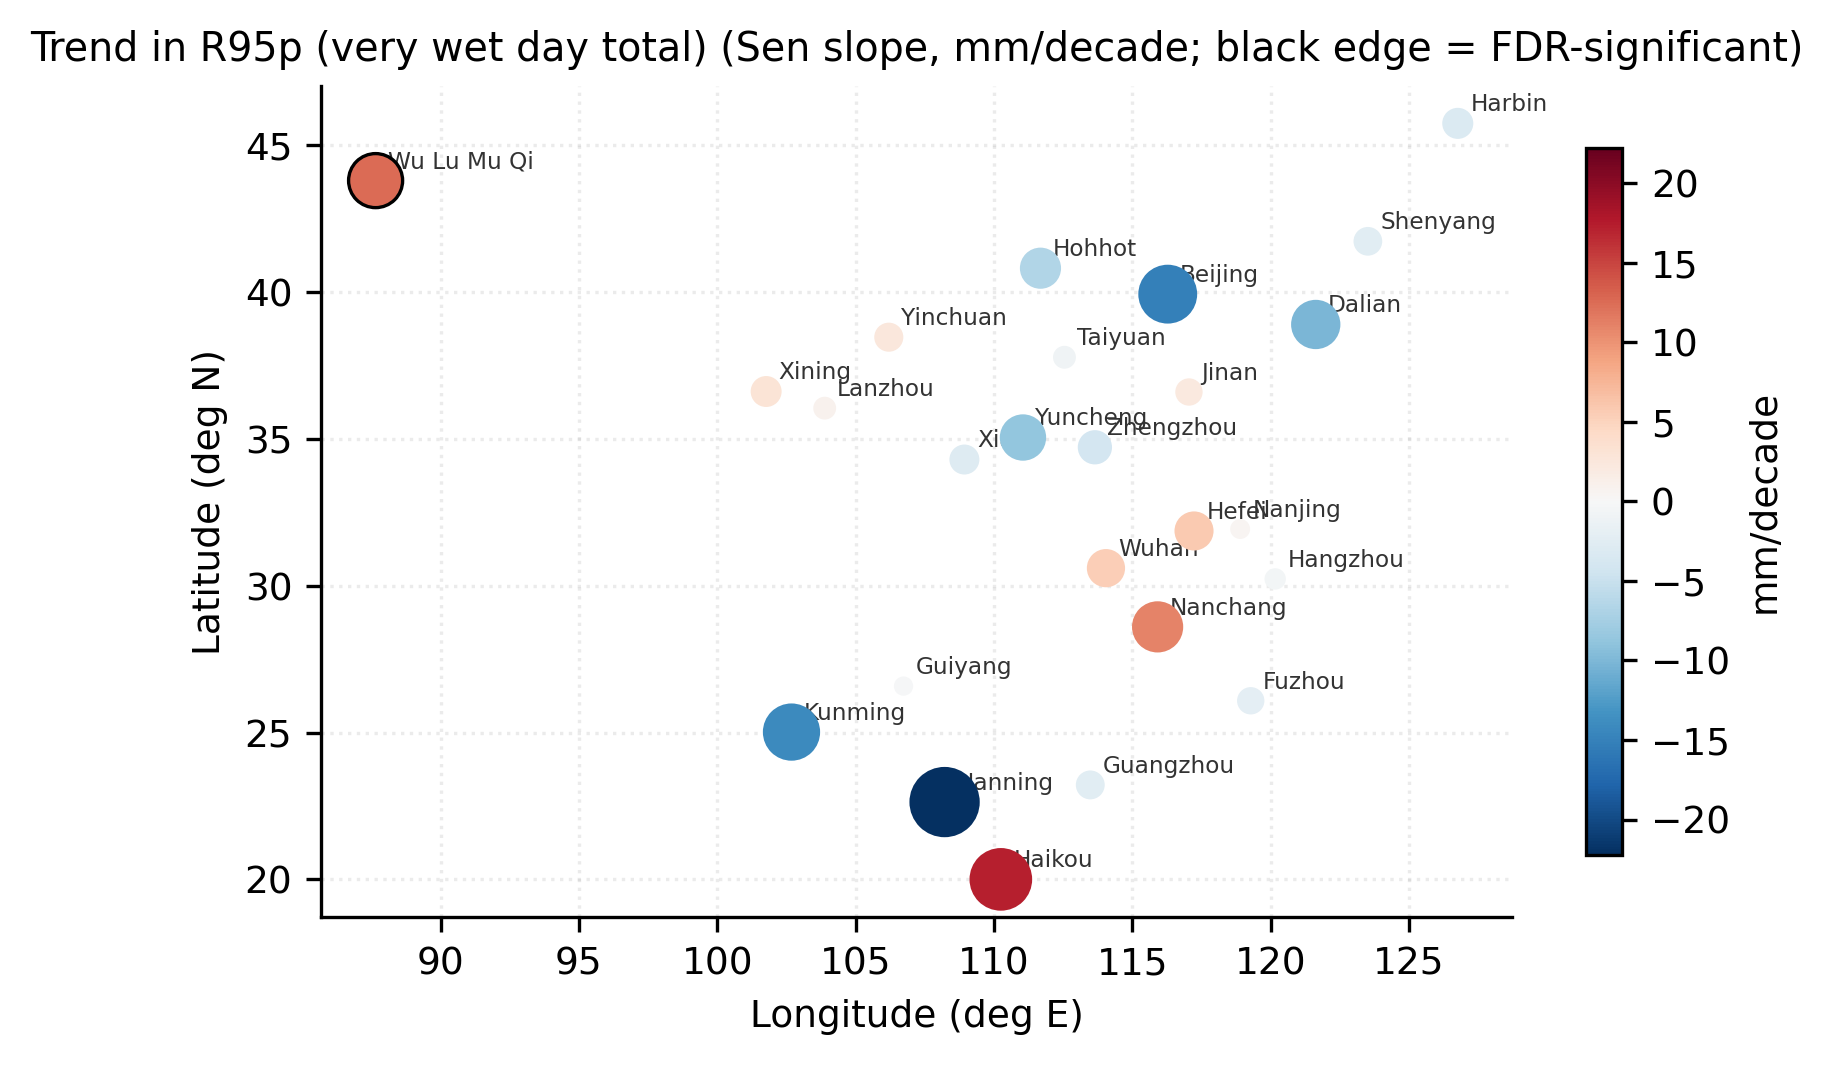
\includegraphics[width=0.62\linewidth]{../02_figures/fig08_trend_map_r95p.png}
\caption{Sen slope of annual R95p (mm per decade) for the national panel; red denotes increasing extreme-rainfall totals.}
\end{figure}

\begin{figure}[H]
\centering
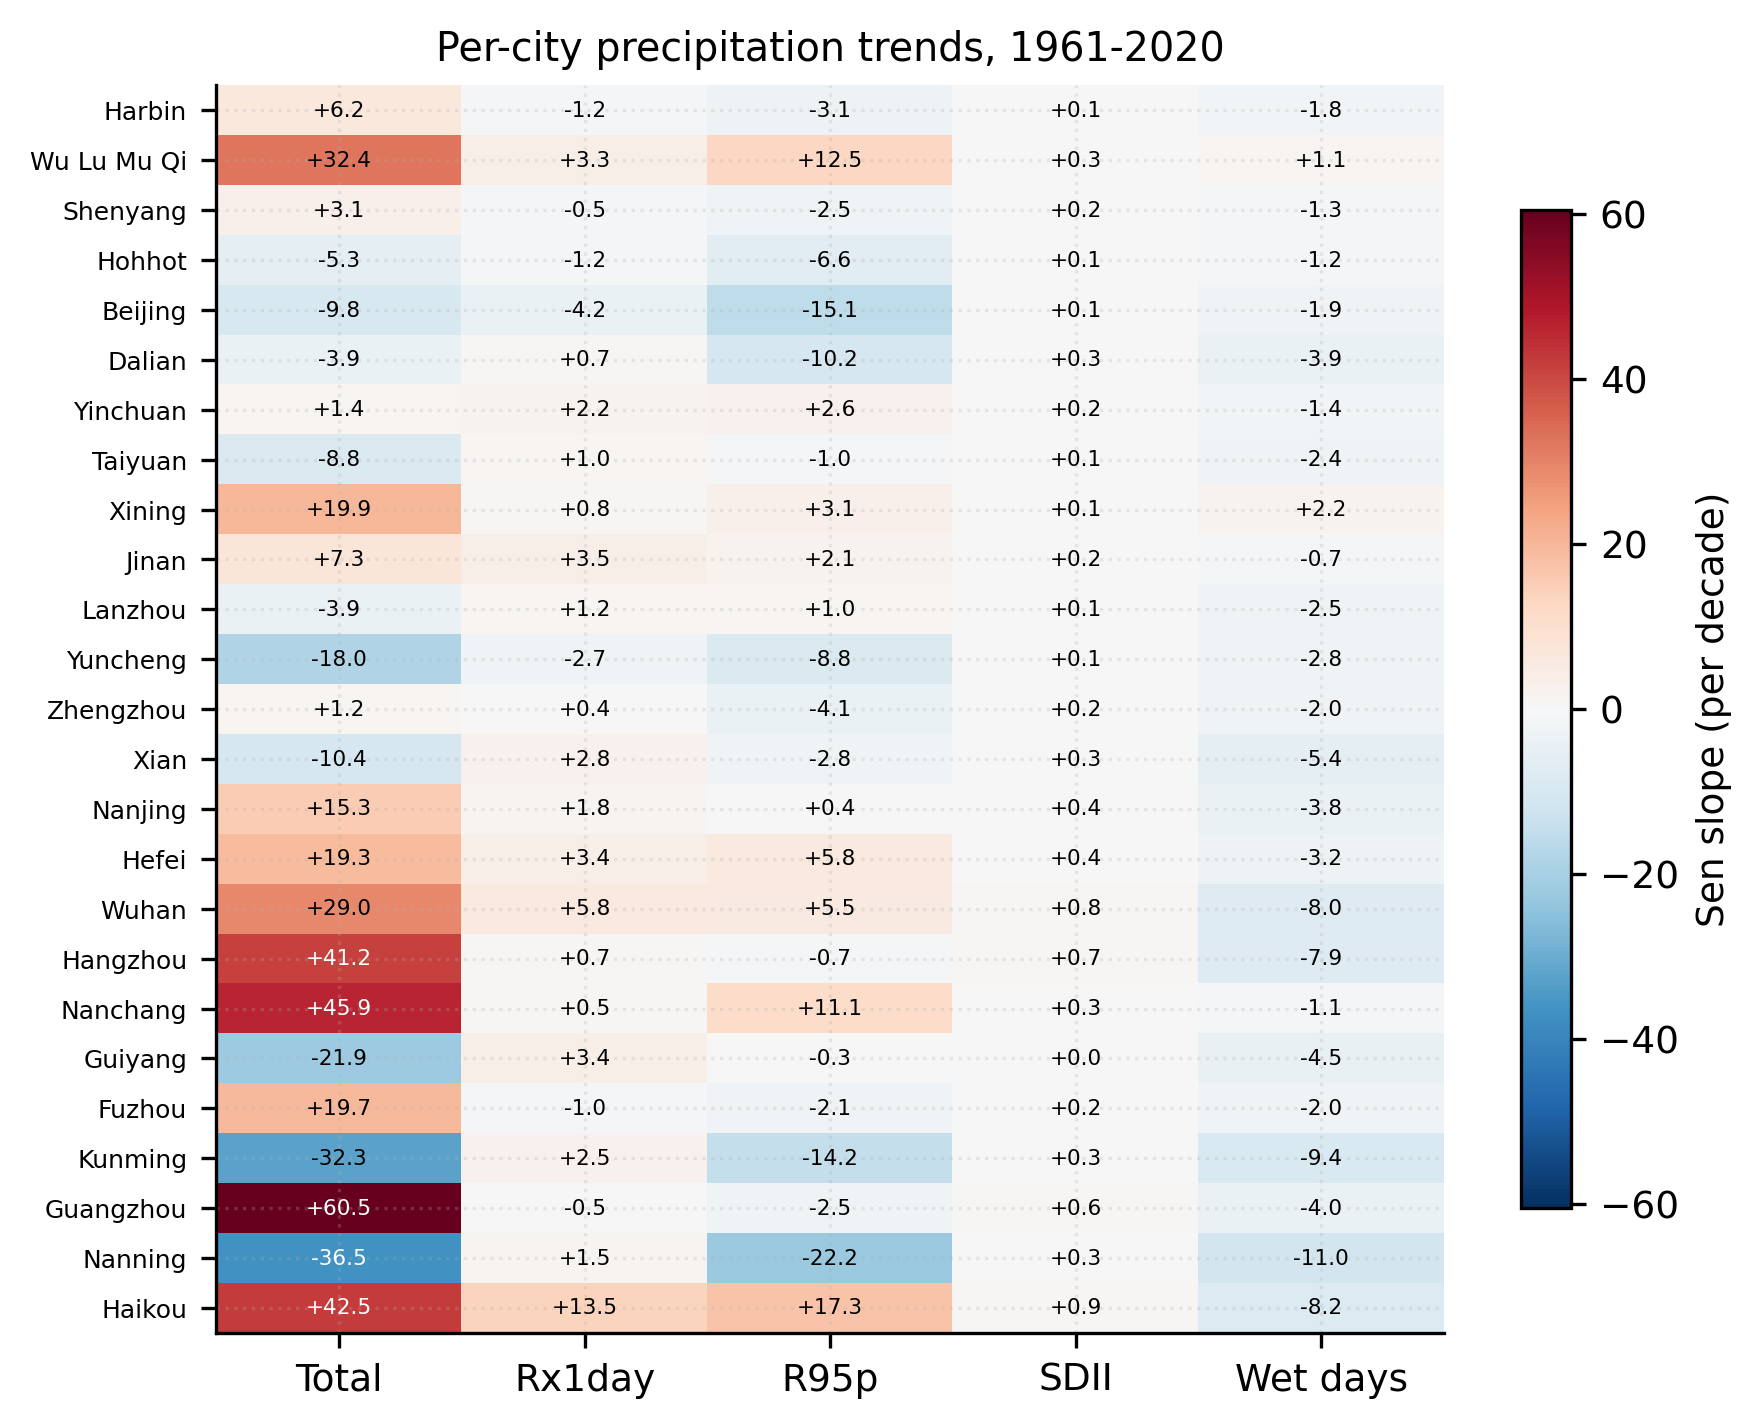
\includegraphics[width=0.62\linewidth]{../02_figures/fig09_trend_heatmap.png}
\caption{City-by-index matrix of Sen slopes, ordered by cluster. Colour is the standardised slope; blank cells are indices with fewer than 45 valid years.}
\end{figure}

\begin{figure}[H]
\centering
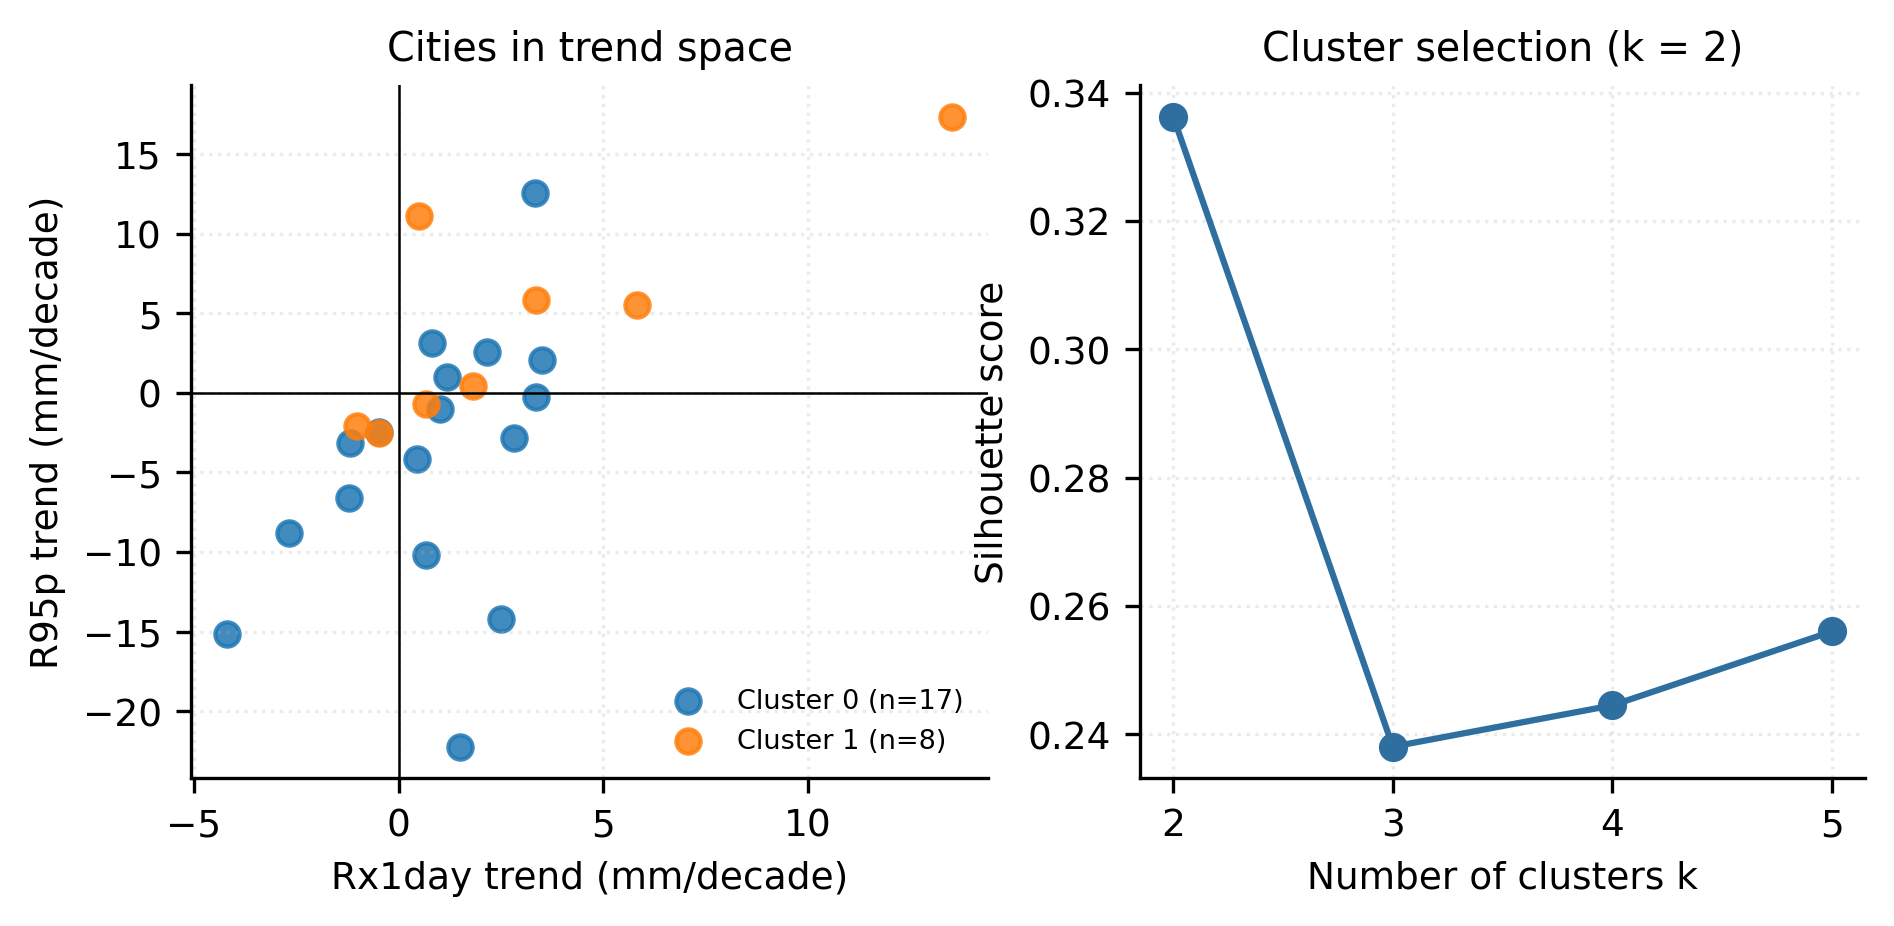
\includegraphics[width=0.56\linewidth]{../02_figures/fig10_clusters.png}
\caption{$k$-means partition of the 25 cities in the space of the first two standardised trend components, with cluster centroids. Silhouette scores: $k=2$, 0.336; $k=3$, 0.238.}
\end{figure}

\begin{figure}[H]
\centering
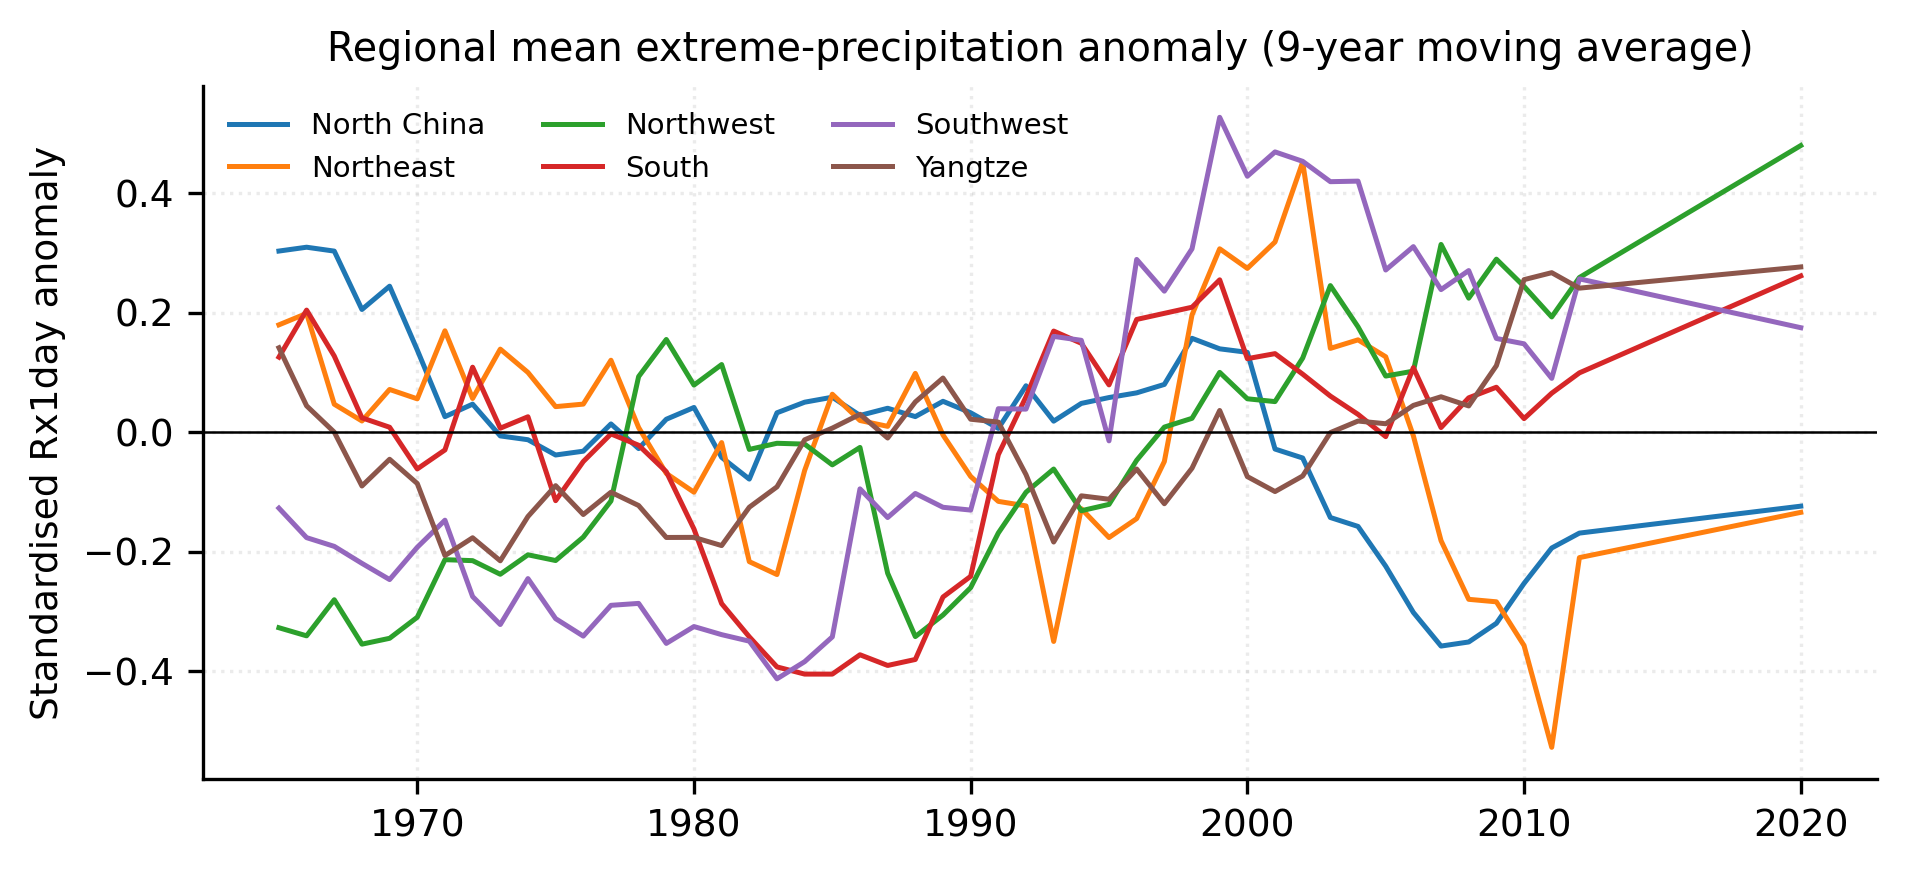
\includegraphics[width=0.62\linewidth]{../02_figures/fig11_regional_anomaly.png}
\caption{Regional standardised anomalies of annual precipitation, smoothed with a five-year running mean. The divergence after 1990 is the regional structure discussed in Section~\ref{sec:q2}.}
\end{figure}

\begin{figure}[H]
\centering
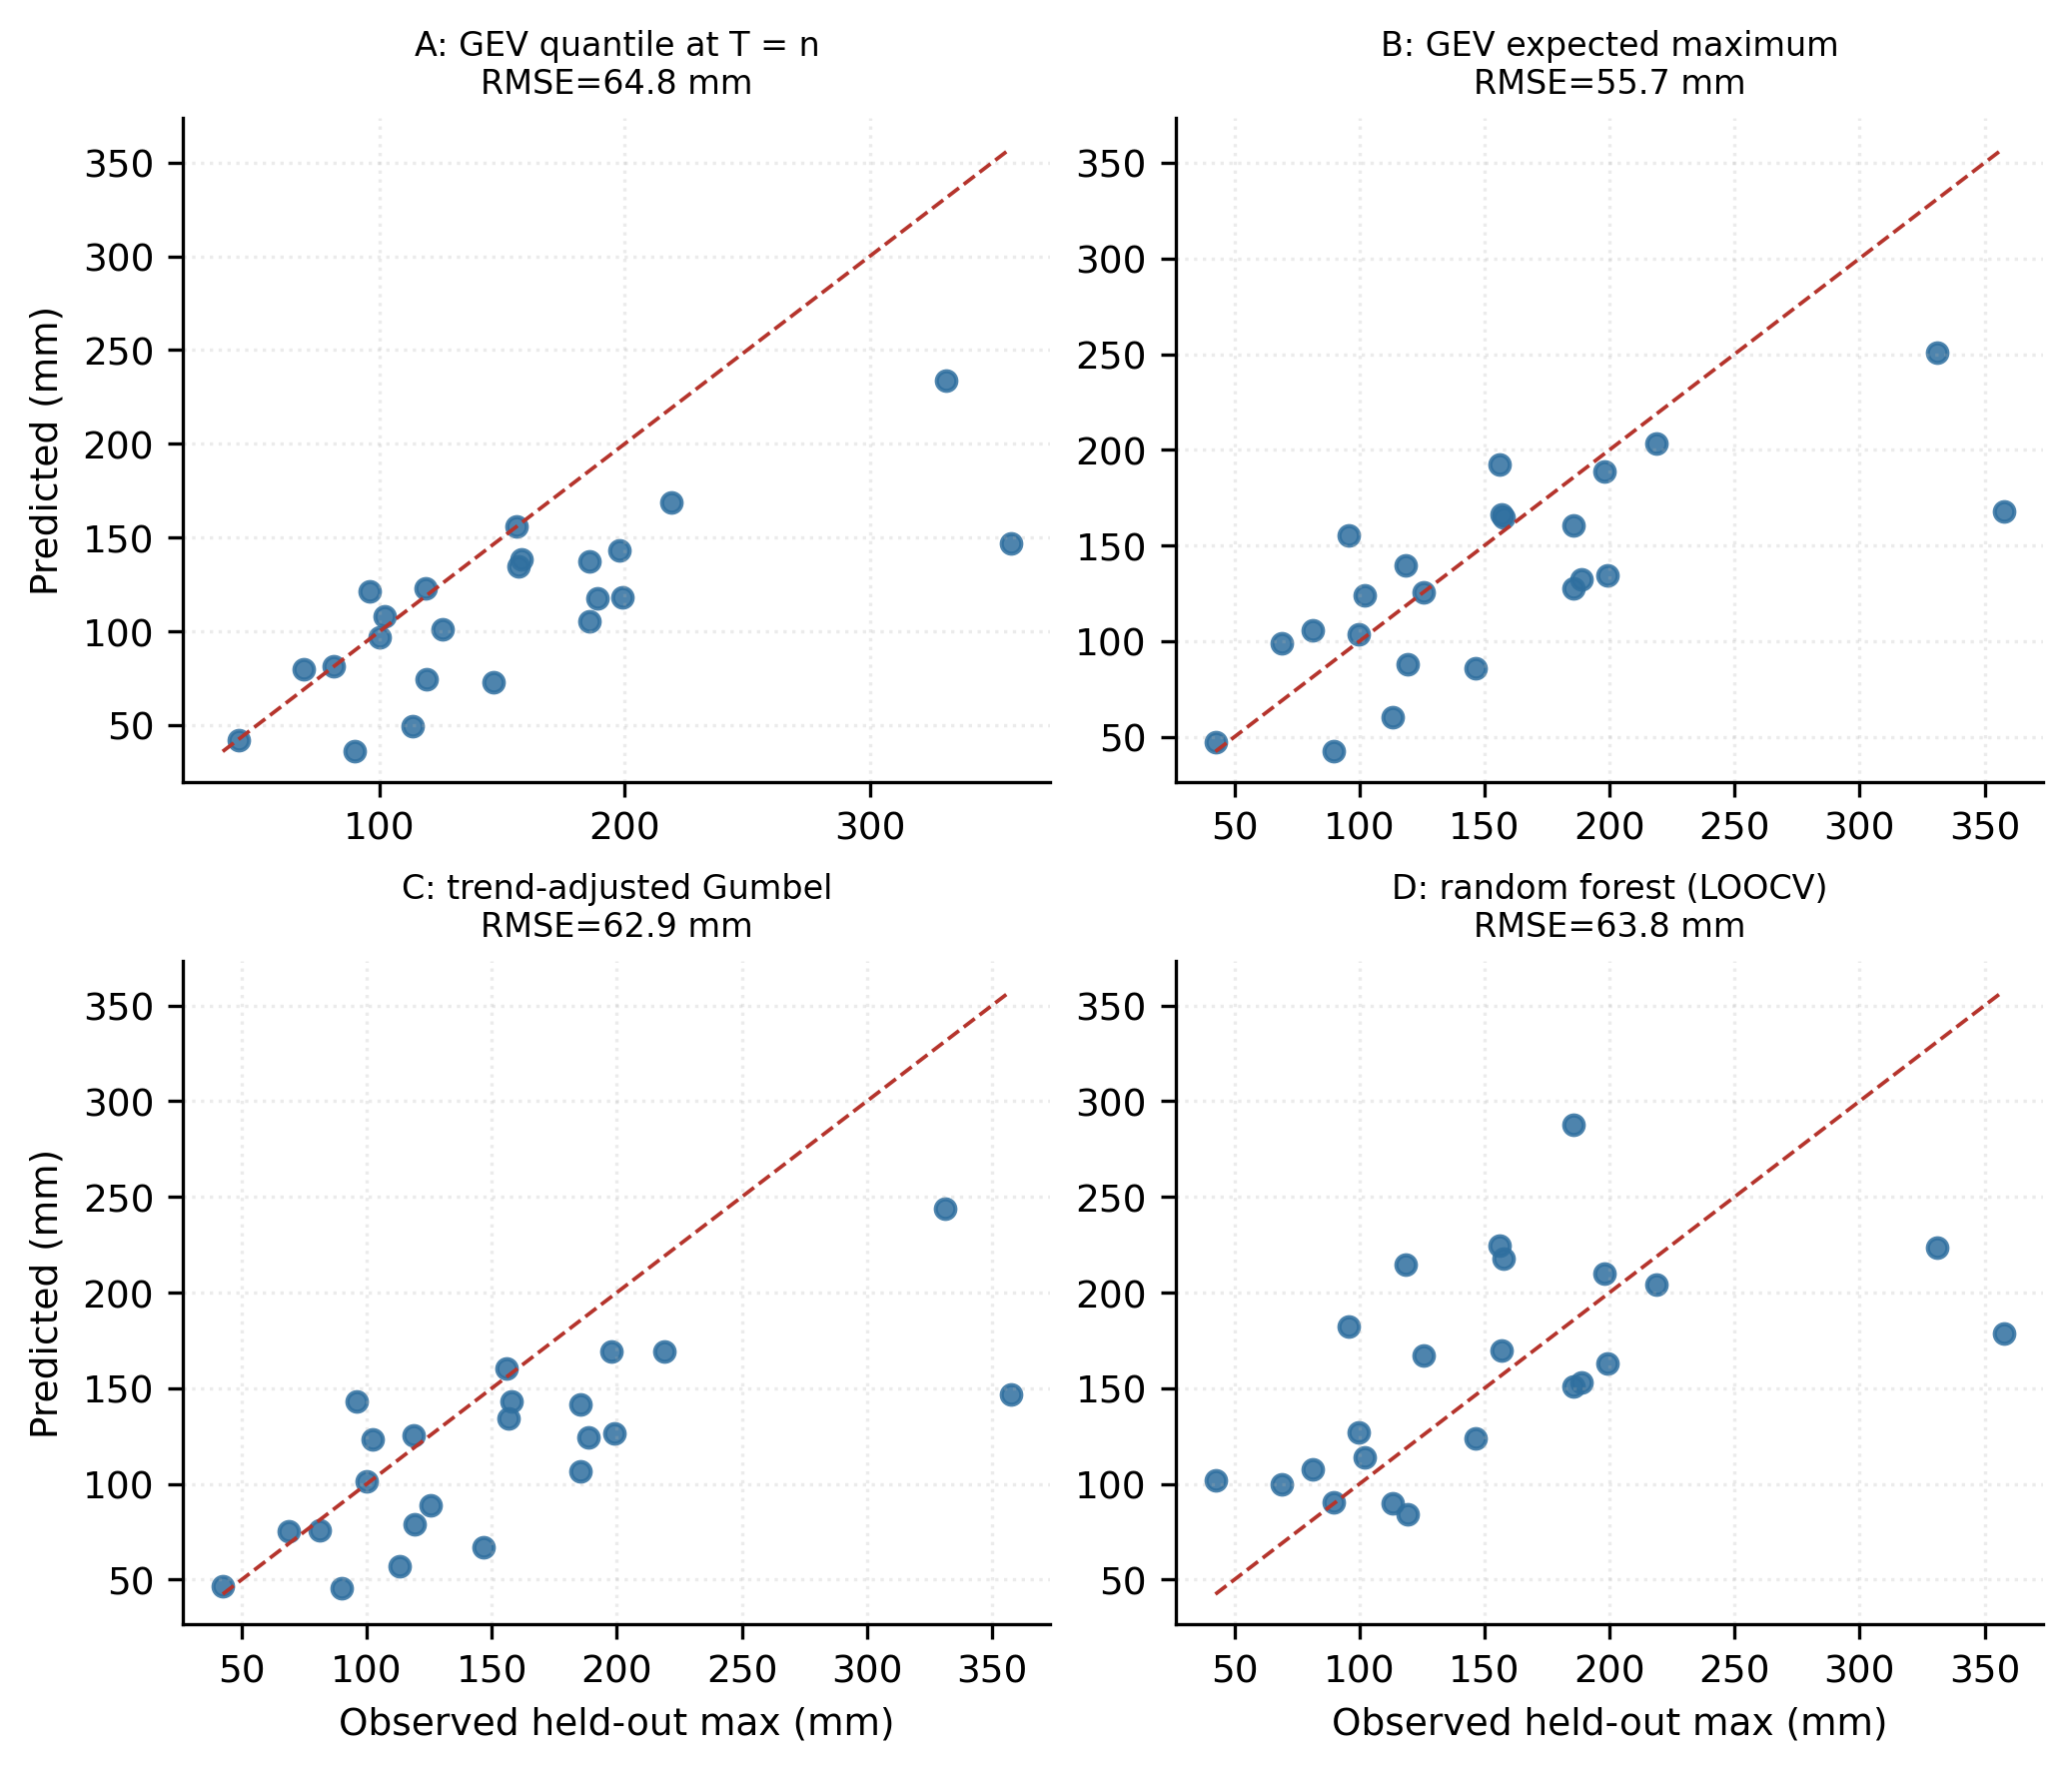
\includegraphics[width=0.62\linewidth]{../02_figures/fig12_method_scatter.png}
\caption{Predicted versus observed held-out maxima for four representative methods. The diagonal is perfect prediction; the horizontal offset of the cloud is the definitional bias of the quantile target.}
\end{figure}

\begin{figure}[H]
\centering
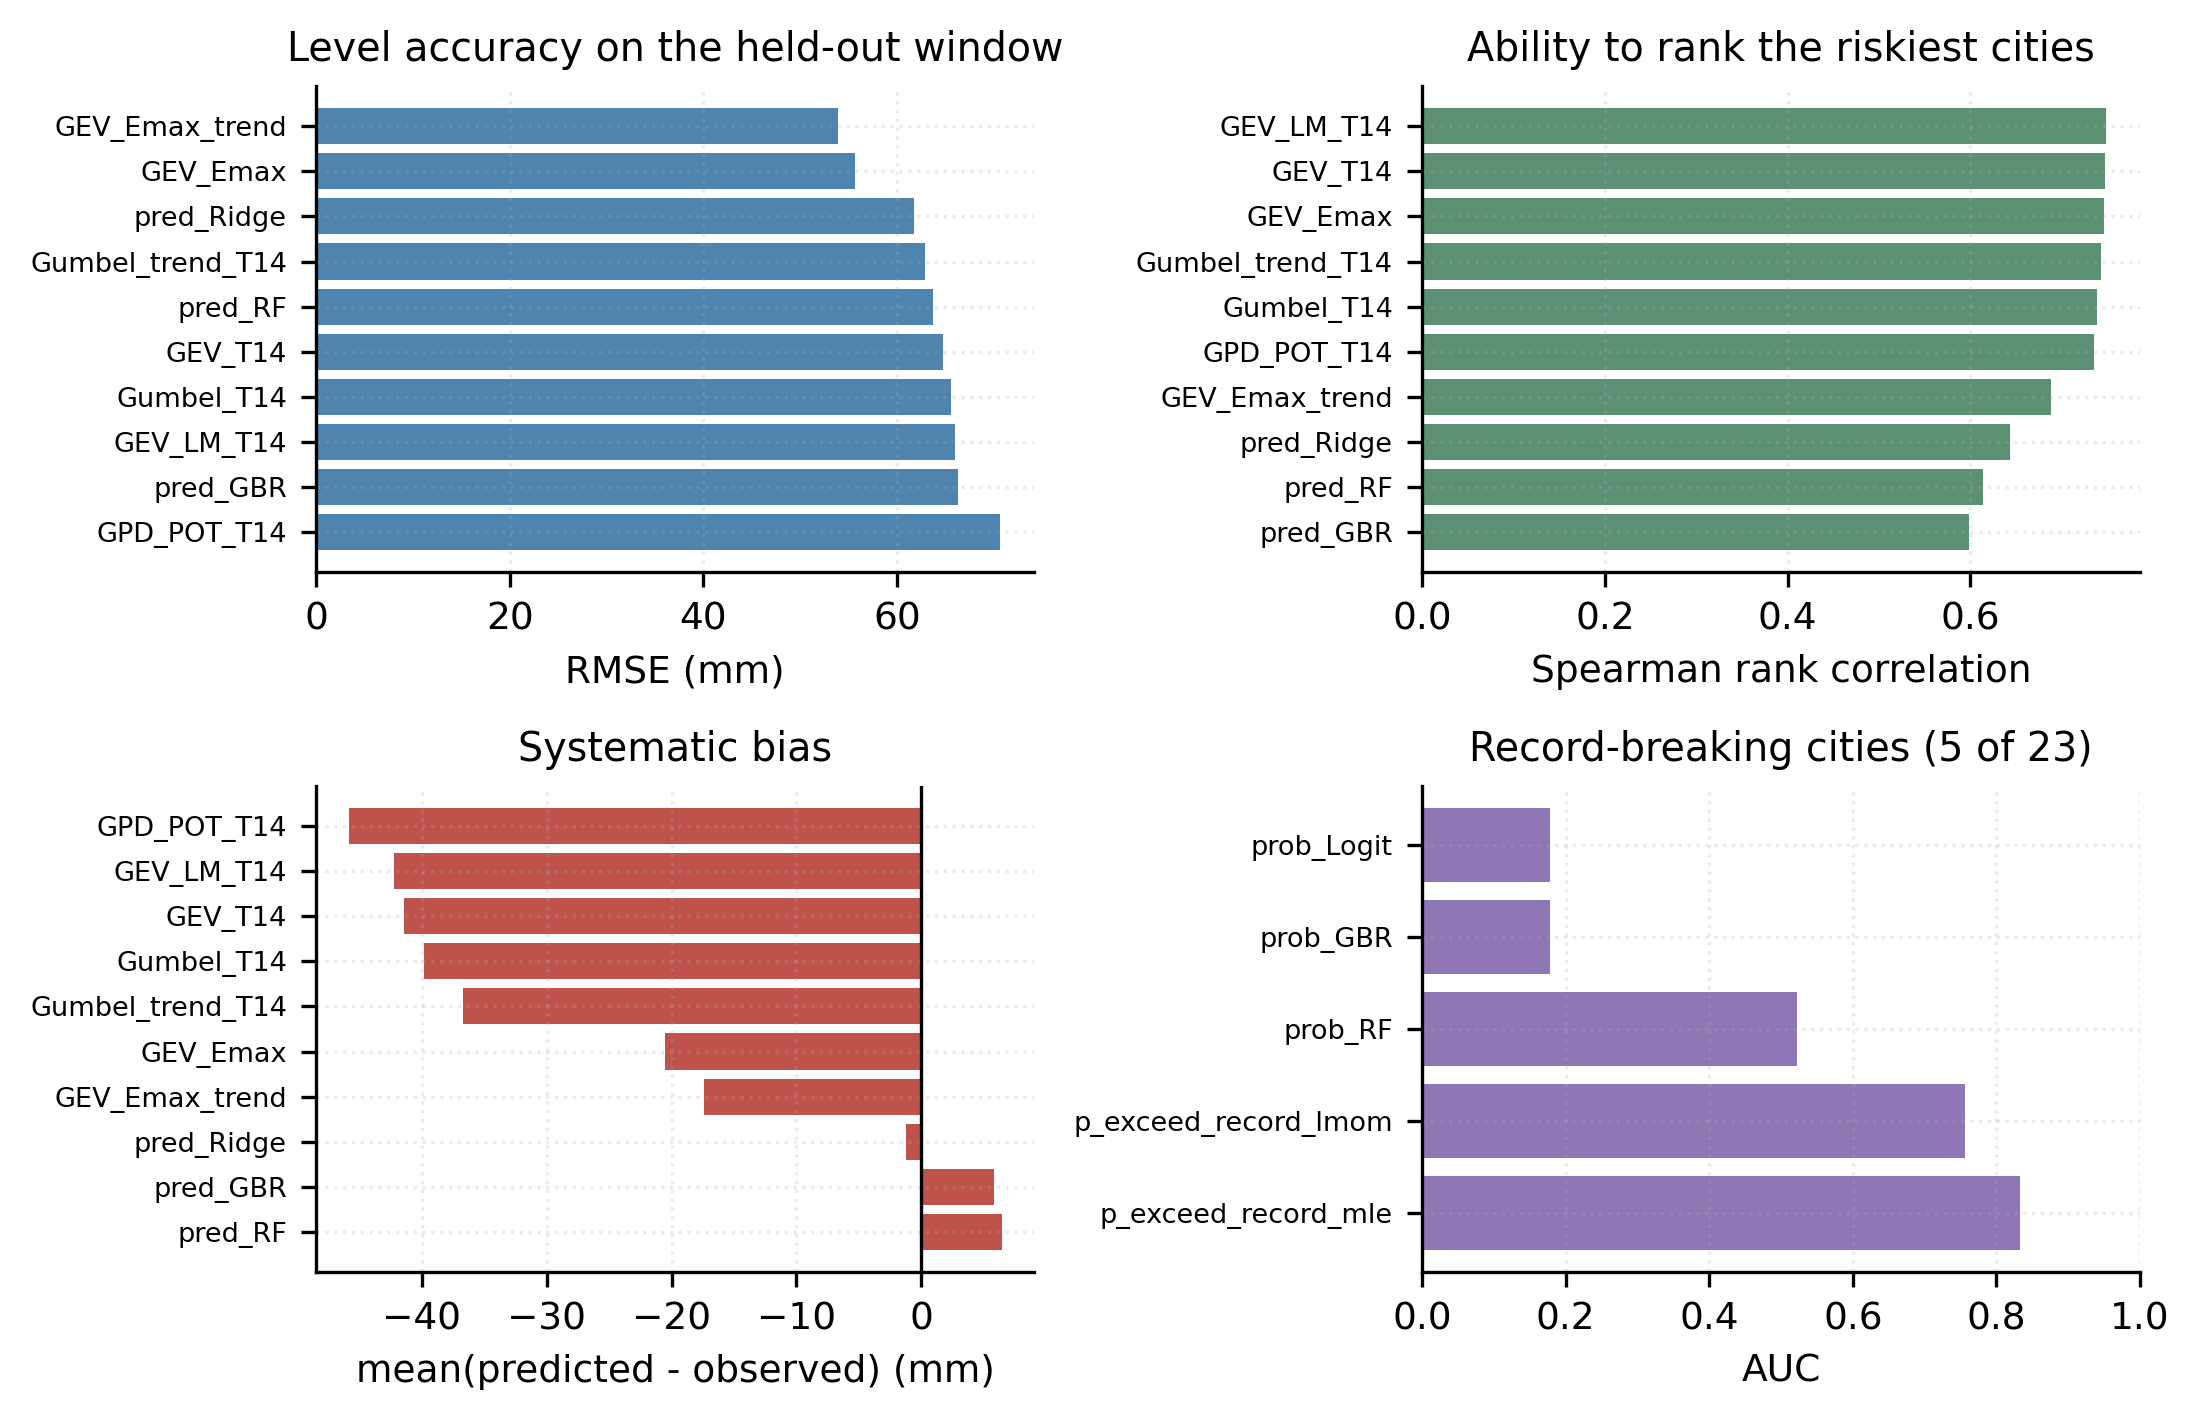
\includegraphics[width=0.62\linewidth]{../02_figures/fig13_method_comparison.png}
\caption{Four criteria for the ten forecast strategies: RMSE, Spearman correlation, bias and, for the classification task, AUC.}
\end{figure}

\begin{figure}[H]
\centering
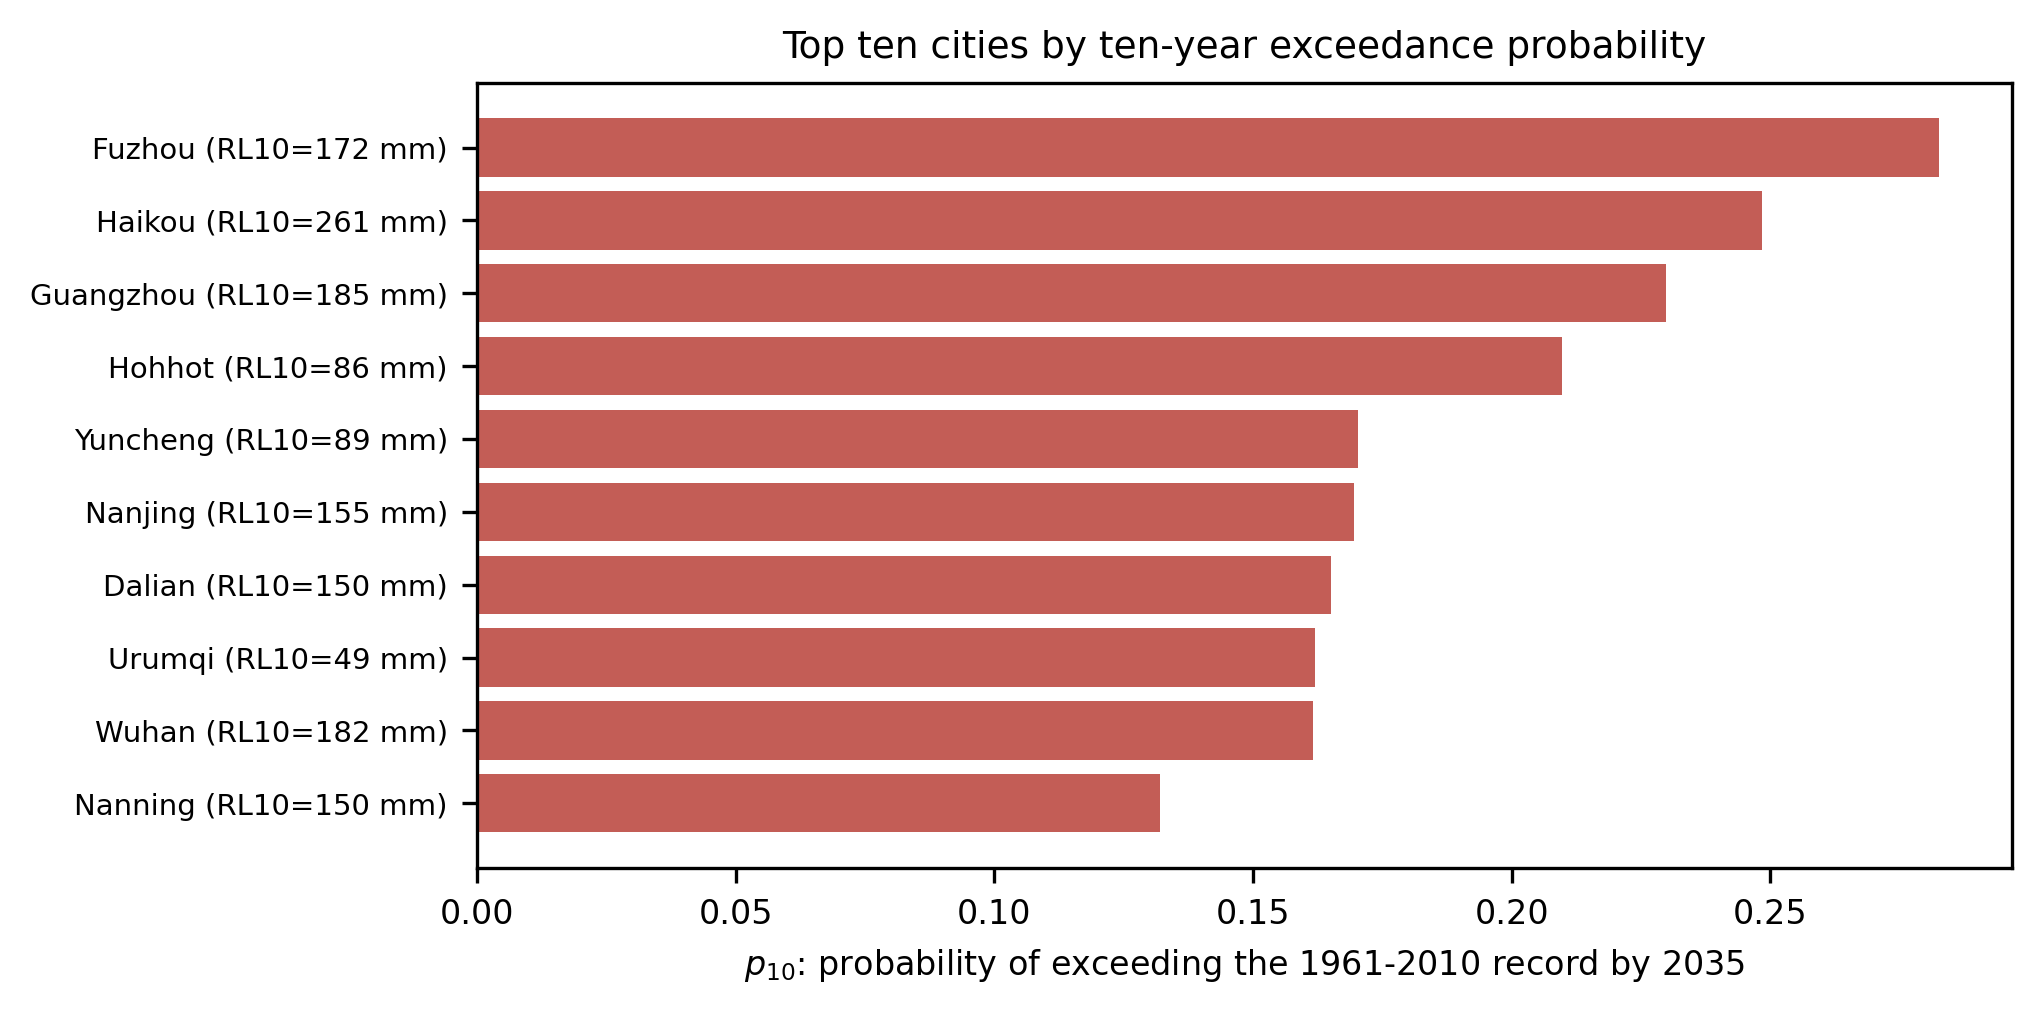
\includegraphics[width=0.58\linewidth]{../02_figures/fig15_risk_ranking.png}
\caption{Ten-year exceedance probability $p_{10}$ of the 1961--2010 record for the ten highest cities, with each city's L-moment ten-year return level in brackets.}
\end{figure}

\begin{figure}[H]
\centering
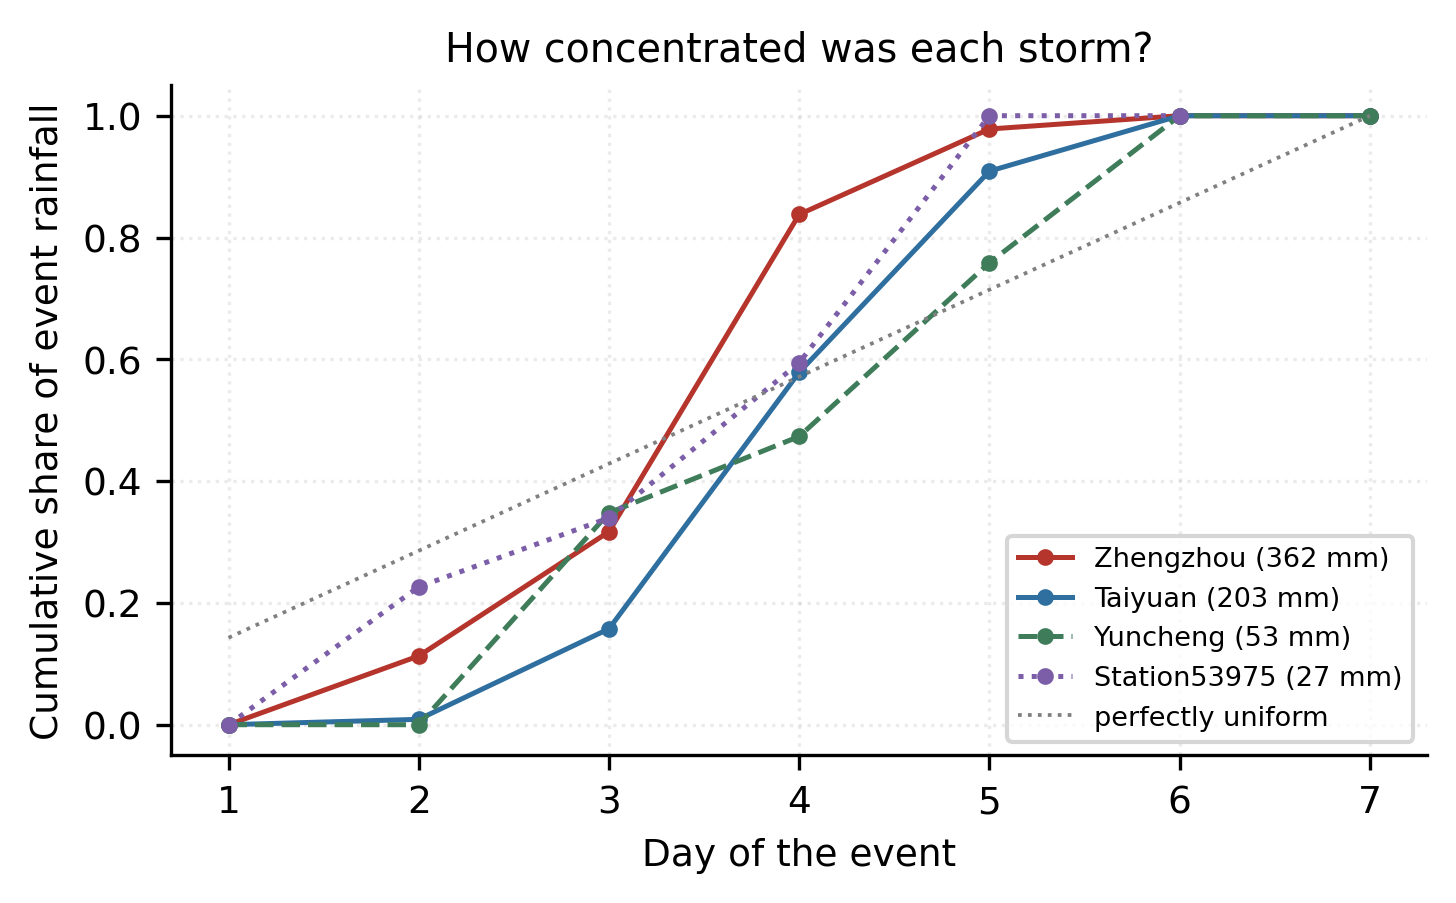
\includegraphics[width=0.62\linewidth]{../02_figures/fig17_concentration.png}
\caption{Cumulative share of event rainfall against elapsed time. The straight diagonal is a perfectly uniform event; Zhengzhou's curve is far above it, Taiyuan's close to it.}
\end{figure}

\begin{figure}[H]
\centering
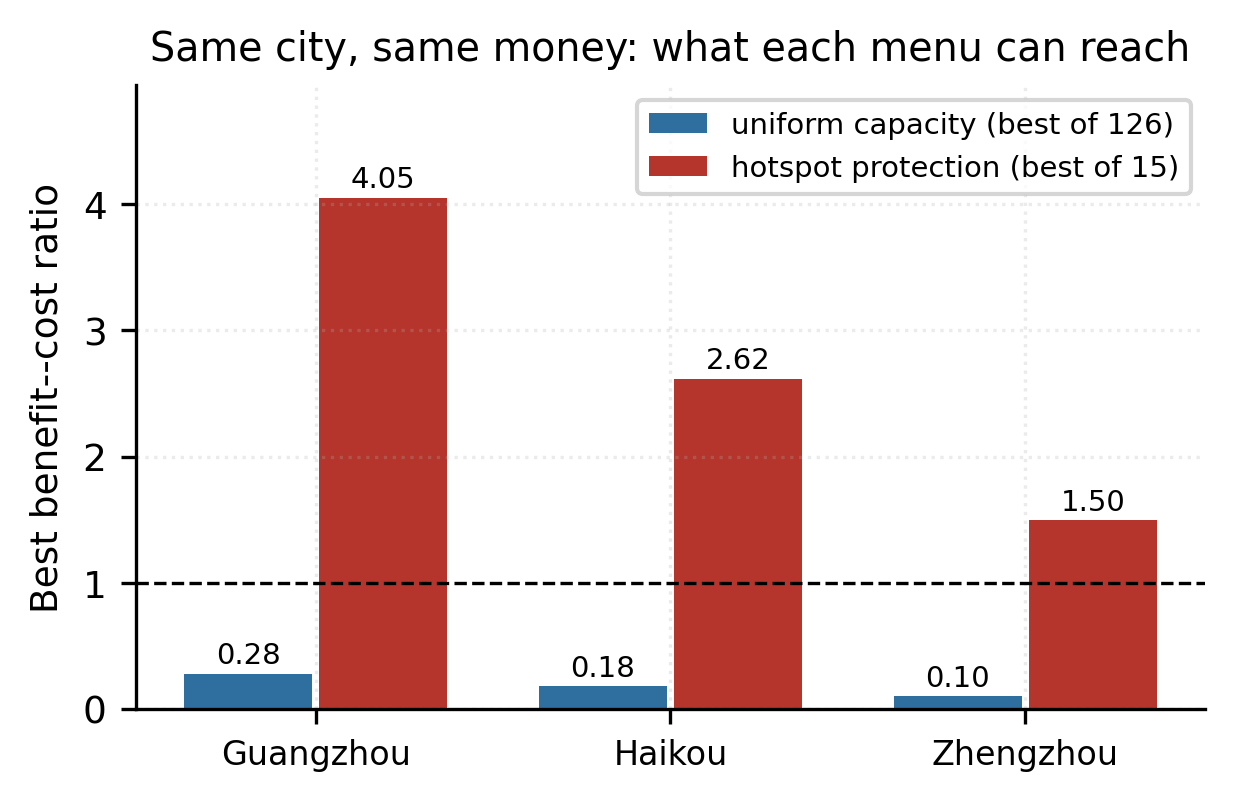
\includegraphics[width=0.60\linewidth]{../02_figures/fig21_bcr.png}
\caption{Best benefit--cost ratio reachable by each menu for the same city: uniform capacity over the 126-point design menu, and hotspot protection over the 15 assumed $(h,m)$ pairs at 5\,mm of local storage. The horizontal line is break-even; no uniform plan reaches it, while every city's hotspot plan does at the favourable pairs.}
\label{fig:bcr}
\end{figure}

\begin{figure}[H]
\centering
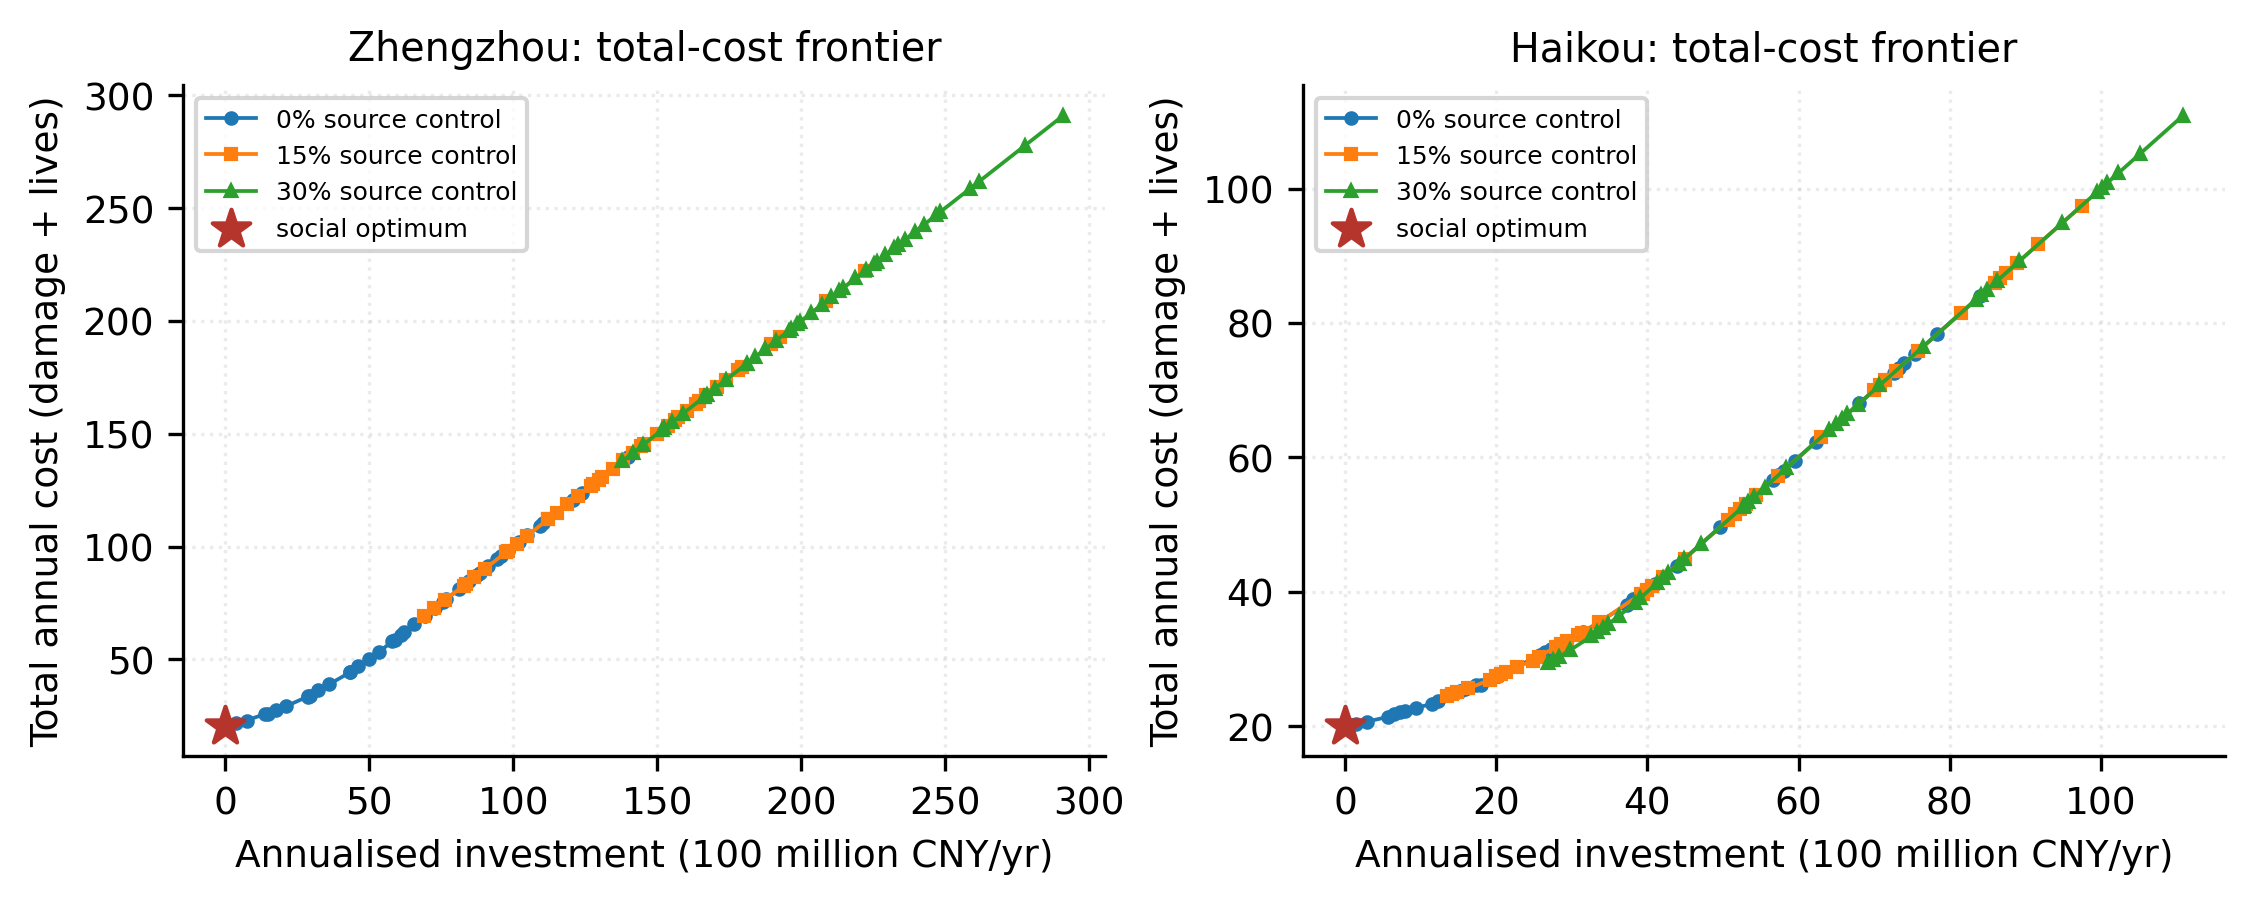
\includegraphics[width=0.60\linewidth]{../02_figures/fig20_cost_damage_frontier.png}
\caption{Total annualised cost (construction amortised over 30 years plus expected residual damage) against annualised investment for Zhengzhou and Haikou. Points on each curve are one plan in the portfolio grid; the star marks the social optimum, not the left edge of the axis.}
\label{fig:frontier}
\end{figure}

\begin{figure}[H]
\centering
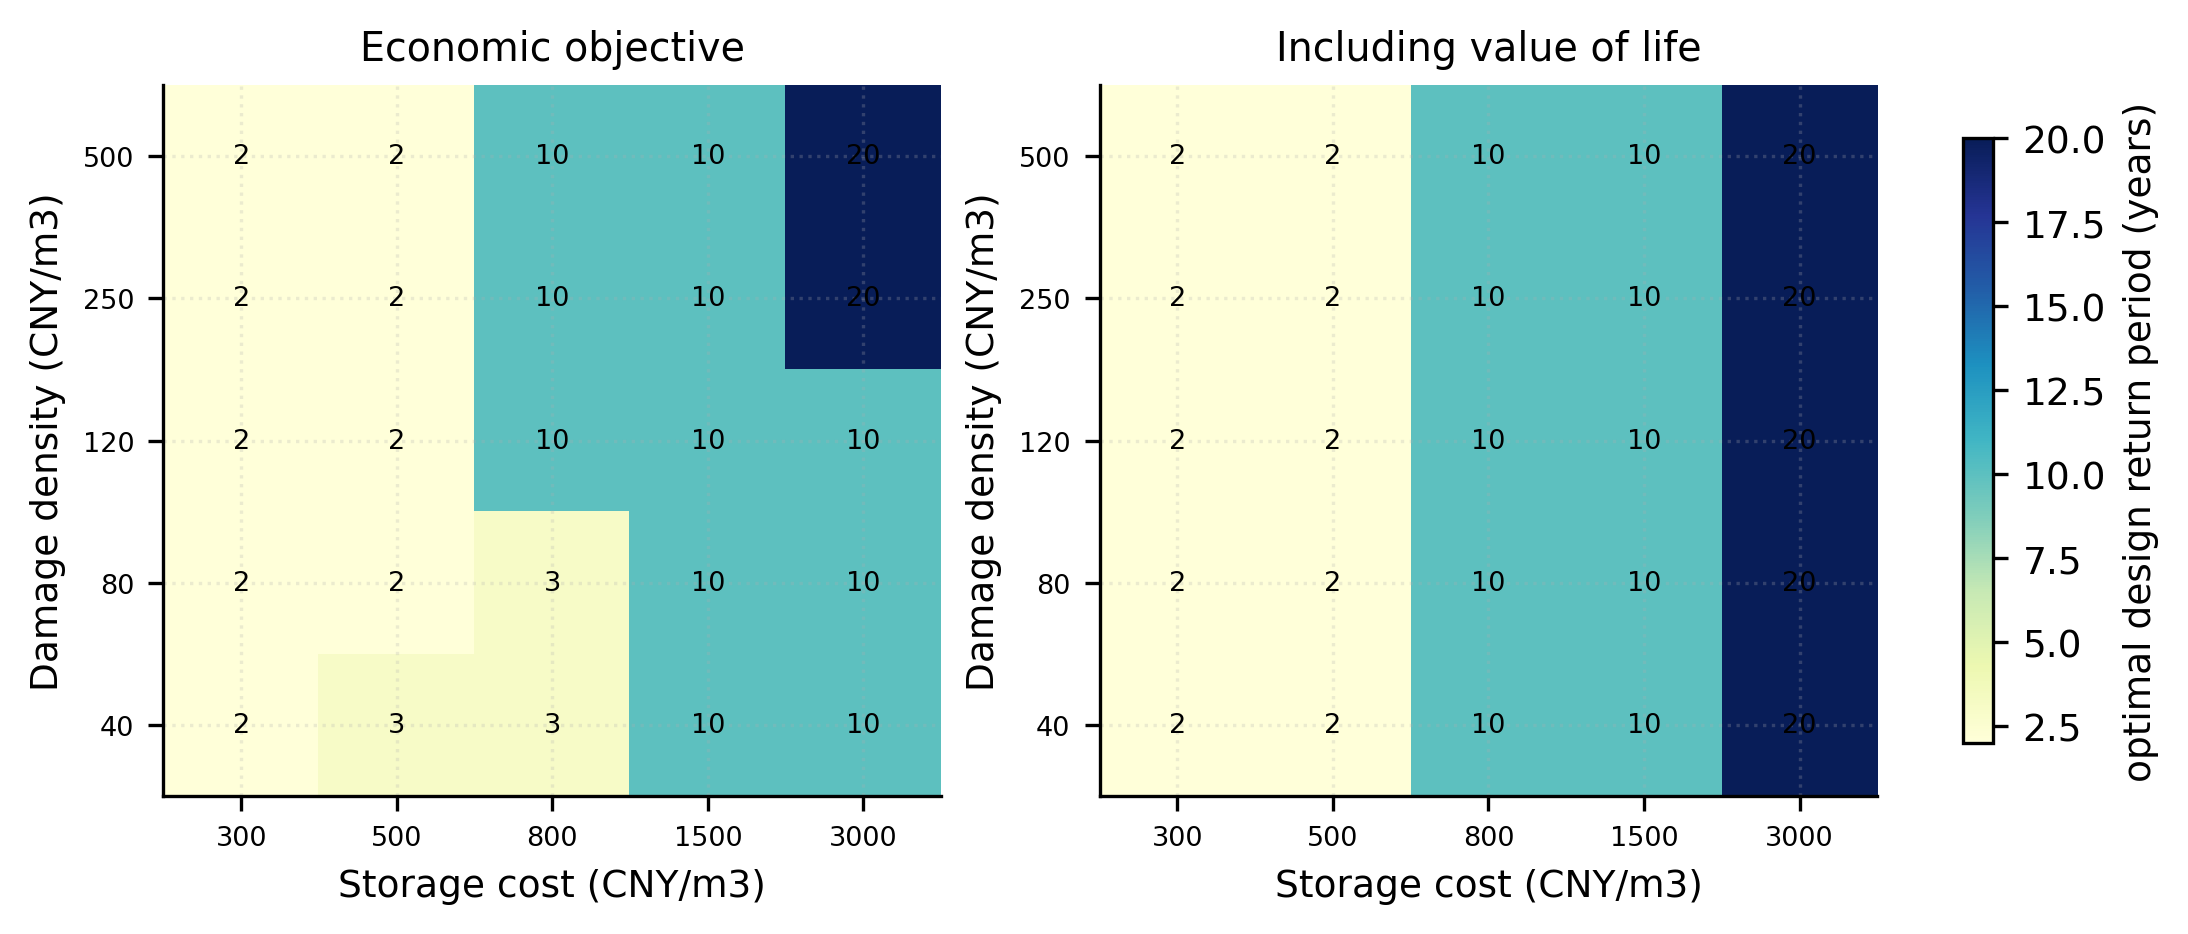
\includegraphics[width=0.60\linewidth]{../02_figures/fig22_sensitivity_tpipe.png}
\caption{Optimal pipe standard against damage density and storage unit cost, under the economic objective (left) and the social objective (right). The standard stays at 2--5 years over most of the space and rises above 10 years only where exposure is extreme and storage expensive.}
\label{fig:senspipe}
\end{figure}

\end{document}